\documentclass[preprint, 10pt]{elsarticle}

%\usepackage{algorithmic}
%\usepackage{algorithm}
\usepackage{amsfonts}
\usepackage[fleqn,reqno]{amsmath}
\usepackage{amssymb}
%\usepackage{amsthm}
\usepackage[titletoc]{appendix}
\usepackage{array}
%\usepackage{bm}
%\usepackage{caption}
%\usepackage[usenames]{color}
\usepackage{enumitem}
%\usepackage{epsfig}
%\usepackage{fancybox}
\usepackage{filecontents}
\usepackage[top=1.2in,bottom=1.2in,left=1in, right=1in]{geometry}
\usepackage{graphics}
%%\usepackage{ifthen}
\usepackage{lineno}
%\usepackage{mathrsfs}
%\usepackage{mdframed}
%\usepackage{multirow}
%\usepackage{palatino}
%\usepackage{showkeys} %To see the labels for now.  Will remove later
%\usepackage{stmaryrd}
%\usepackage{subfigure}
%\usepackage{paralist}
\usepackage{pgfplots}
%\usepackage{tabularx}
\usepackage{tikz}
\usepackage{todonotes}
\usetikzlibrary{arrows}
\usepackage{comment}

%%%%%%  pdftex  %%%%%%%%%%%%%%%%%%%%%%%%%%%%%%%%%%%%%%%%%%%%%%%%%%%%%%
\usepackage[pagebackref=false,bookmarks=false]{hyperref} 

\hypersetup{
  bookmarksnumbered=true,
  bookmarksopen=false,
  hypertexnames=false,      
  breaklinks=true,          
  unicode=false,
  pdffitwindow=true,        
  pdfnewwindow=true,        
  colorlinks=true,         
  linkcolor=dblue,
  anchorcolor=red,
  citecolor=dorange,
  filecolor=magenta,
  urlcolor=dblue,
  pdfstartview = FitH,
  pdfkeywords = {},
  pdfcreator = {LaTeX with hyperref package}
}



\newcommand{\bd}{{\partial}}
\newcommand{\bigO}{{\mathcal{O}}}
\newcommand{\cc}{{\mathbf{c}}}
\newcommand{\DD}{{\mathcal{D}}}
\newcommand{\eeta}{{\boldsymbol\eta}}
\newcommand{\ff}{{\mathbf{f}}}
\newcommand{\grad}{{\nabla}}
\newcommand{\II}{{\mathbf{I}}}
\newcommand{\iin}{\mathrm{in}}
\newcommand{\llambda}{{\boldsymbol\lambda}}
\newcommand{\nn}{{\mathbf{n}}}
\newcommand{\NN}{{\mathcal{N}}}
\newcommand{\out}{\mathrm{out}}
\newcommand{\rr}{{\mathbf{r}}}
\newcommand{\RR}{{\mathbb{R}}}
\renewcommand{\ss}{{\mathbf{s}}}
\newcommand{\ssigma}{{\boldsymbol\sigma}}
\newcommand{\tar}{\mathrm{tar}}
\newcommand{\uu}{{\mathbf{u}}}
\newcommand{\UU}{{\mathbf{U}}}
\newcommand{\vv}{{\mathbf{v}}}
\newcommand{\xx}{{\mathbf{x}}}
\newcommand{\xxi}{{\boldsymbol{\xi}}}
\newcommand{\yy}{{\mathbf{y}}}

\def\gap{\hspace*{.2in}}

% Derivatives
\newcommand{\pderiv}[2]{\frac{\partial #1}{\partial #2}}
\newcommand{\tderiv}[2]{\frac{d #1}{d #2}}
\newcommand{\ppd}[2]{\frac{\partial^2 #1}{{\partial #2}^2}}

% Nick's commands
\newcommand{\vsp}[1]{\vspace{#1 pc} \noindent}
\newcommand{\abs}[1]{\lvert #1 \rvert}
\newcommand{\mean}[1]{\left< #1 \right>}
\newcommand{\thL}{$\theta$--$L$}
\newcommand{\eps}{\varepsilon}
\newcommand{\Vn}{V_n}
\newcommand{\Vs}{V_s}
\newcommand{\atau}{\abs{\tau}}
\newcommand{\thalpha}{\pderiv{\theta}{\alpha}}
\newcommand{\elfun}{\zeta}
\newcommand{\thhat}{\hat{\theta}}
\newcommand{\Dt}{\Delta t}
\newcommand{\NLterm}{\mathcal{N}}
\newcommand{\Mterm}{\mathcal{M}}
\newcommand{\FourierSum}{ \sum_{k = -N_\iin /2}^{N_\iin /2-1} }
\newcommand{\atausig}{\atau^{(\sigma)}}
\newcommand{\Vnsig}{\Vn^{(\sigma)}}
\newcommand{\Vssig}{\Vs^{(\sigma)}}


\newcommand{\tauD}[1]{\tau_{#1\text{D}}}
\newcommand{\atauD}[1]{\abs{\tau_{#1\text{D}}}}

\usepackage{showkeys}
\begin{document}

\title{Viscous Transport in Eroding Porous Media}


% OTHER TITLE POSSIBILITIES
% ???

\author[SH]{Shang-Huan Chiu}
\author[Nick]{M.~N.~J.~Moore}
\author[Bryan]{Bryan D.~Quaife}

\address[SH]{Department of Scientific Computing, Florida State
University, Tallahassee, FL, 32306.}
\address[Nick]{Department of Mathematics and Geophysical Fluid Dynamics
Institute, Florida State University, Tallahassee, FL, 32306.}
\address[Bryan]{Department of Scientific Computing and Geophysical Fluid
Dynamics Institute, Florida State University, Tallahassee, FL, 32306.}

\begin{abstract} 
  An abstract
\end{abstract}

\begin{keyword}
  Keyword 1 \sep Keyword 2 \sep Keyword 3 
\end{keyword}

\maketitle

%%%%%%%%%%%%%%%%%%%%%%%%%%%%%%%%%%%%%%%%%%%%%%%%%%%%%%%%%%%%%%%%%%%%%%%
\section{Introduction}
\label{sec:intro}
%%%%%%%%%%%%%%%%%%%%%%%%%%%%%%%%%%%%%%%%%%%%%%%%%%%%%%%%%%%%%%%%%%%%%%%
Flow in many natural occurring geometries involves flows that vary over
many orders of magnitude.  \todo[]{The grammar in the first sentence is awkward: Flow in ... involves flows?}
For example, the length scales of a porous
media can vary from $10^{-6}m$ to
$10^{-1}m$~\cite{mil-chr-imh-mcb-ped1998}.  Porous media flow plays an
important role in several environmental and industrial applications.
Therefore, understanding the dynamics of pore-scale flow is central to
upscale the governing fluid equations, characterize
dispersion~\cite{saf1959}, and quantify mixing. However, because of the
large disparity of length and velocity scales, constitutive laws that
link the microscopic scale to macroscopic scale must be
developed~\cite{mil-chr-imh-mcb-ped1998}.  Therefore, to find closure
formulas, accurate simulations at microscopic scales must be performed
and analyzed.  A few examples of closure formulas and coarse-grained
variables include
pressure-saturation-permeability~\cite{mil-chr-imh-mcb-ped1998},
permeability-porosity~\cite{dar-mcc1998, car1937, won-kop-tom1984},
first passage time distribution~\cite{ber-sch-sil2000,
hym-den-hag-kan2019, cve-che-wen1996}, tortuosity~\cite{hak-com-den2019,
mat-kha-koz2008, dud-koz-mat2011, kop-kat-tim1996}, concentration
distributions~\cite{ica-den2019, bel-sal-rin1992}, flow
distributions~\cite{ali-par-wei-bre2017}, geometry
connectivity~\cite{knu-car2005, wes-blo-gra2001}, pore
distributions~\cite{ali-par-wei-bre2017}, and anomalous
dispersion~\cite{dea-qua-bir-jua2018, den-cor-sch-ber2004,
sie-ili-pri-riv-gua2019}.

In many applications, the fluid transport continuously changes the pore
structure.  This is particularly common in geophysical flows where
erosion alters the porous matrix.  In this work, we investigate flow in
eroded porous media.  By introducing erosion, there is a two-way
coupling between the hydrodynamics and the mechanical alteration of the
complex porous geometry.  Transport in porous geometries that have
undergone erosion finds applications in aquifers~\cite{cve-che-wen1996,
sud1986}, solute transport in groundwater flow~\cite{dag1987,
kon-bre1978}.  Porous geometries that have undergone erosion have
certain characteristics.  For example, the geometry often has regions of
high porosity that connect the inlet to the outlet.  This channelization
results in velocity scales that can vary over several orders of
magnitude~\cite{all-hea-lab-rei2002}.  Moreover, the channelization
results in a geometry that is largely heterogeneous and anisotropic, and
this affects heat transfer through the medium~\cite{nil-sto1990,
ree-sto1995}.  Others have studied transport in heterogeneous geometries
(for example, see~\cite{mil-chr-imh-mcb-ped1998, ber-sch-sil2000,
hak-com-den2019, suo-liu-gan2019, cus-hu-den1995, cve-che-wen1996,
leb-ded-dav-bou2007, knu-car2005, bel-sal-rin1992}). However, to the
best of our knowledge, a detailed study of transport in eroded
geometries has not been performed.

To describe the relevant hydrodynamics, we model two-dimensional
microscopic scales where the fluid is governed by the incompressible
Stokes equations (for example, see~\cite{hym-den-hag-kan2019,
den-ica-hid2018, bar-mar-vee-zha2018}).  To couple the erosion and the
hydrodynamics, the grains of the porous media are eroded at a rate that
is proportional to the hydrodynamic shear stress~\cite{wan-fel2004,
ris-moo-chi-she-zha2012, qua-moo2018, par-izu2000}.  A variety of
numerical methods can be applied to solve the incompressible Stokes
equations such as a lattice-gas or lattice Boltzmann
model~\cite{kop-kat-tim1996, dar-mcc1998}, finite
volume~\cite{suo-liu-gan2019, den-ica-hid2018, sie-ili-pri-riv-gua2019},
finite differences~\cite{leb-ded-dav-bou2007, knu-car2005}, and cellular
automata~\cite{rot1988}. In this work, we instead solve an equivalent
boundary integral equation (BIE) formulation of the incompressible
Stokes equation.  The BIE is discretized with a high-order quadrature
method that resolves nearly touching bodies with a near-singular
integration scheme~\cite{bar-wu-vee2015}.  The erosion dynamics are
simulated by applying a stable second-order time stepping Runge-Kutta
method to the {\thL} formulation~\cite{hou-low-she1994} of the eroding
bodies.  Given the solution of the incompressible Stokes equations are
solved in an eroded porous geometry, we investigate different metrics to
characterize transport.  We focus on three metrics: the tortuosity, the
anomalous dispersion, and the distribution of geometrical channels.  

The first two of these metrics can be defined in terms of statistical
moments of trajectories.  Depending on the application, transport at the
microscale can be modelled as pure advection~\cite{dea-qua-bir-jua2018,
leb-ded-dav-bou2007, cve-che-wen1996, puy-gou-den2019}, and advection
dispersion equation~\cite{cus-hu-den1995, dag1987, den-ica-hid2018}, or
with a random walk~\cite{saf1959, bij-blu2006, ber-sch-sil2000}.  In
this work, we assume that the trajectories are governed purely by
advection (ie.~no diffusion).  Therefore, a trajectory $\ss(t)$
initialized at $\ss_0$ is governed by
\begin{align}
  \frac{d\ss}{dt} = \uu(\ss,t), \quad \ss(0) = \ss_0,
  \label{eqn:tracers}
\end{align}
where $\uu$ is the fluid velocity.  Since there is no diffusion, all
dispersion is a result of the particle spreading induced by the porous
geometry.  Since there is no diffusion, we apply a high-order explicit
Runge-Kutta time stepping method to compute streamlines.  However, other
groups have simulated trajectories using continuous time random
walks~\cite{mon-wei1965, den-cor-sch-ber2004, leb-den-car2008,
ber-cor-den-sch2006} and a Fokker-Planck equation~\cite{ica-den2019}.

\todo[inline]{Dump of text}
Resolving the flow in these small velocity regions is essential to
accurately describe anomalous dispersion and
mixing~\cite{leb-den-dav-bol-car-dec-bou2011, den-leb-eng-bij2011}.
\todo[inline]{Dump of text}


In a porous geometry, the length of a particle path is larger than the
distance travelled if the grains were absent.  To quantify the amount of
winding a particle takes, we use the tortuosity that is defined as the
ratio of the particle paths length to the distance between the inlet and
outlet.  In fractured media, the local tortuosity can be over
2.5~\cite{hym-den-hag-kan2019}, and in porous media, depending on the
porosity, the local tortuosity can be greater than
1.5~\cite{kop-kat-tim1996, mat-kha-koz2008}, or greater than
2~\cite{dud-koz-mat2011}.  The tortuosity of the geometry is defined by
averaging over the entire inlet.  Therefore, the geometry's tortuosity
can be used to characterize average particle
motions~\cite{hak-com-den2019}.

The tortuosity is a first statistical moment of the streamlines.
However, to measure spread of trajectories, second-order moments are
computed. By computing the variance of the lengths of trajectories in a
porous media, non-local anomalous dispersion is
observed~\cite{kan-dea-nun-bij-blu-jua2014, cus-hu-den1995,
dea-leb-den-tar-bol-dav2013}, resulting in super-dispersion.  The
dispersion depends on the amount of time trajectories spend in low and
high velocity regimes~\cite{ber-sch2001}.  Anomalous dispersion has been
investigated for a variety of porous geometries, but not in the context
of eroding porous geometries.

Rather than solving the fluid equations in a complex porous matrix,
network models can be used to describe the flow.  Here, the pores
between neighboring grains are thought of as small channels, and the
geometry consists of a connected network of these
channels~\cite{bry-kin-mel1993, bry-mel-cad1993, bij-blu2006} with the
flow resembling a Hagen-Poiseuille profile in each channel.  So that
network models can be applied to an eroding geometry, we characterize
the pore sizes between neighboring grains as a function of the
geometry's porosity.  The pore size distribution can be used to quantify
velocity distributions~\cite{ali-par-wei-bre2017, dea-qua-bir-jua2018},
channelization~\cite{sie-ili-pri-riv-gua2019}, and
connectivity~\cite{knu-car2005, wes-blo-gra2001}.

The numerical methods to solve the governing fluid and erosion equations
are based on previous work of the authors~\cite{qua-moo2018}.  We
continue to use a boundary integral equation (BIE) formulation of the
incompressible Stokes equations and a second-order Runge-Kutta method
applied to a smoothed version of the magnitude of the shear stress.  In
our previous work, we discretized the BIE with the trapezoid rule whose
accuracy grows when evaluating layer potentials close to the fluid
boundary.  Therefore, given a fixed resolution, our previous work
required a minimum separation distance between all bodies to maintain
stability.  One of the earliest works on near-singular integration was
developed by Baker and Shelley~\cite{bak-she1986}, and in recent years,
many other near-singular integration schemes have been
developed~\cite{oja-tor2015, kli-tor2018, hel-oja2008a, bea-yin-wil2016,
bea-lai2001, klo-bar-gre-one2013}.  In this work, we use a Barycentric
quadrature method~\cite{bar2014, bar-wu-vee2015} since it is a
non-intrusive modification of the trapezoid rule, and the error is
guaranteed to be uniformly bounded.  In this work, we extend this
quadrature method so that it can be used to compute the gradient of the
velocity which is required to compute the shear stress and the fluid
vorticity.

\begin{figure}[H]
\begin{center}
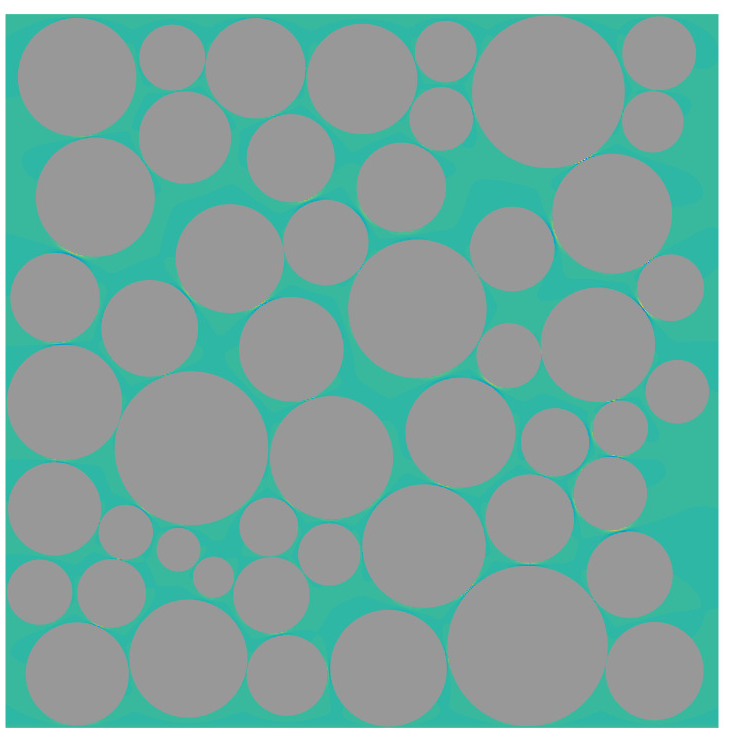
\includegraphics[width = 0.3 \textwidth]{./figs/vort_50b1}
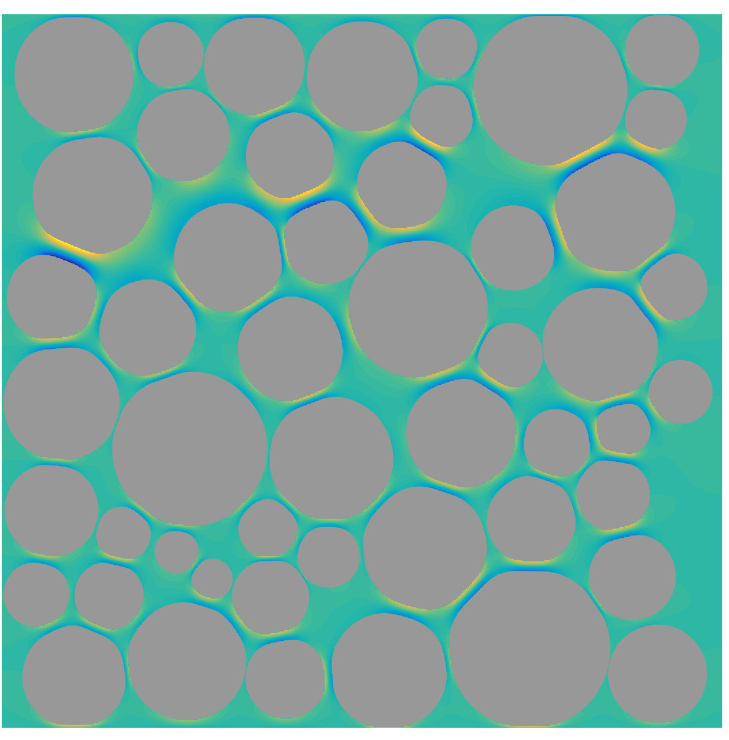
\includegraphics[width = 0.3 \textwidth]{./figs/vort_50b80}
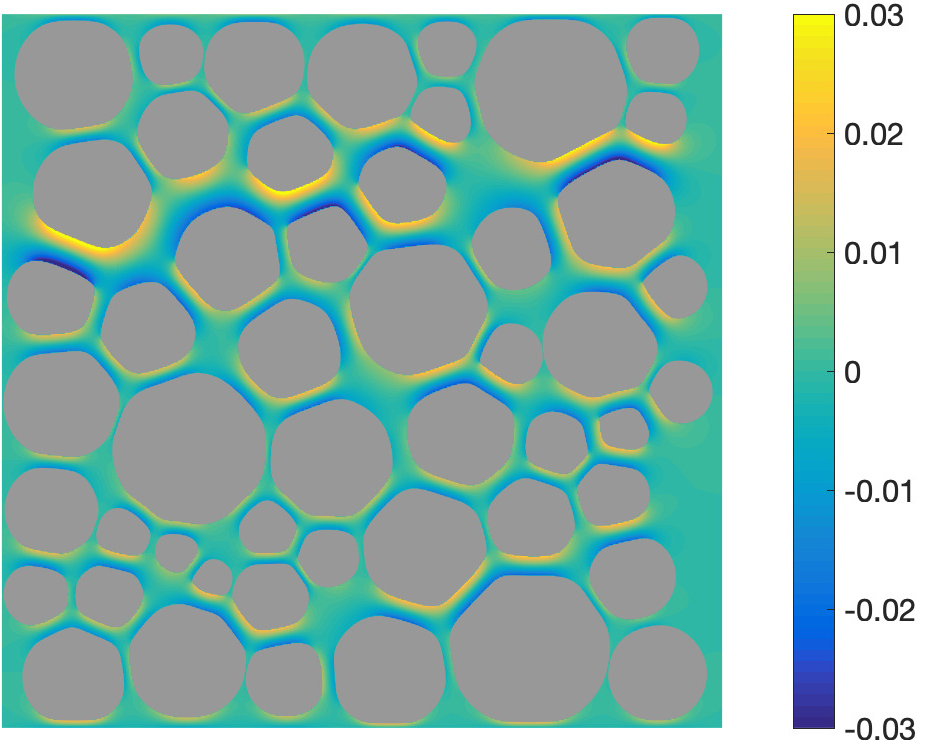
\includegraphics[width = 0.38 \textwidth]{./figs/vort_50b160}\\
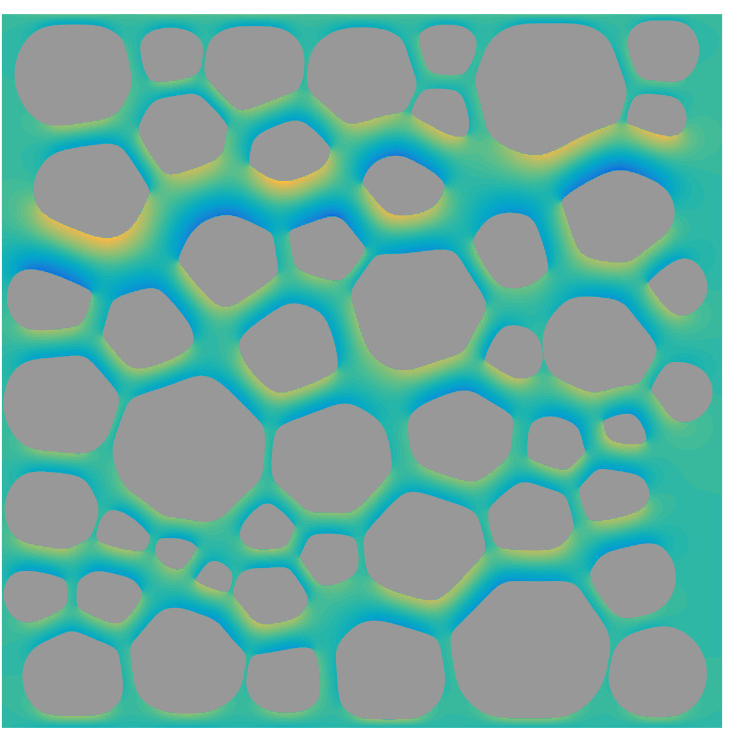
\includegraphics[width = 0.3 \textwidth]{./figs/vort_50b240}
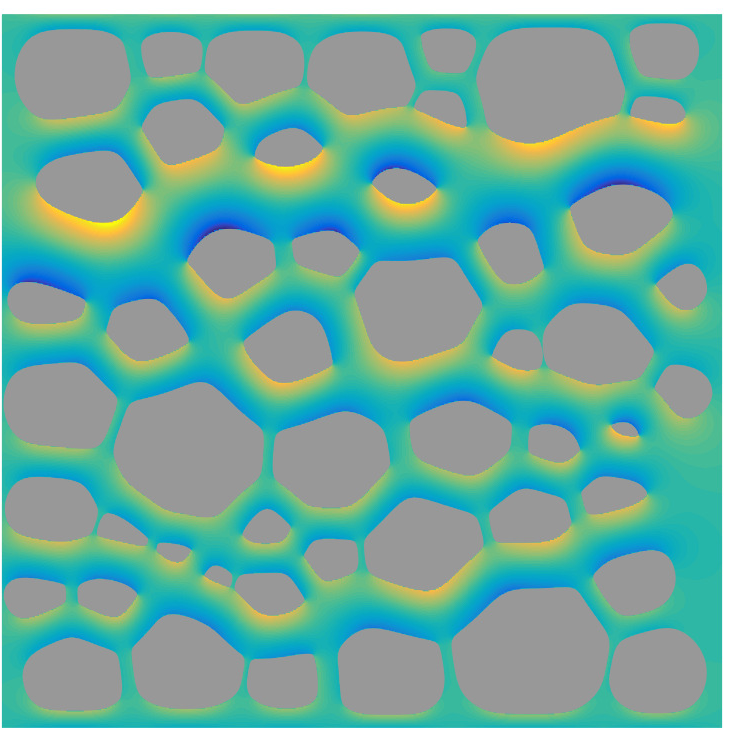
\includegraphics[width = 0.3 \textwidth]{./figs/vort_50b320}
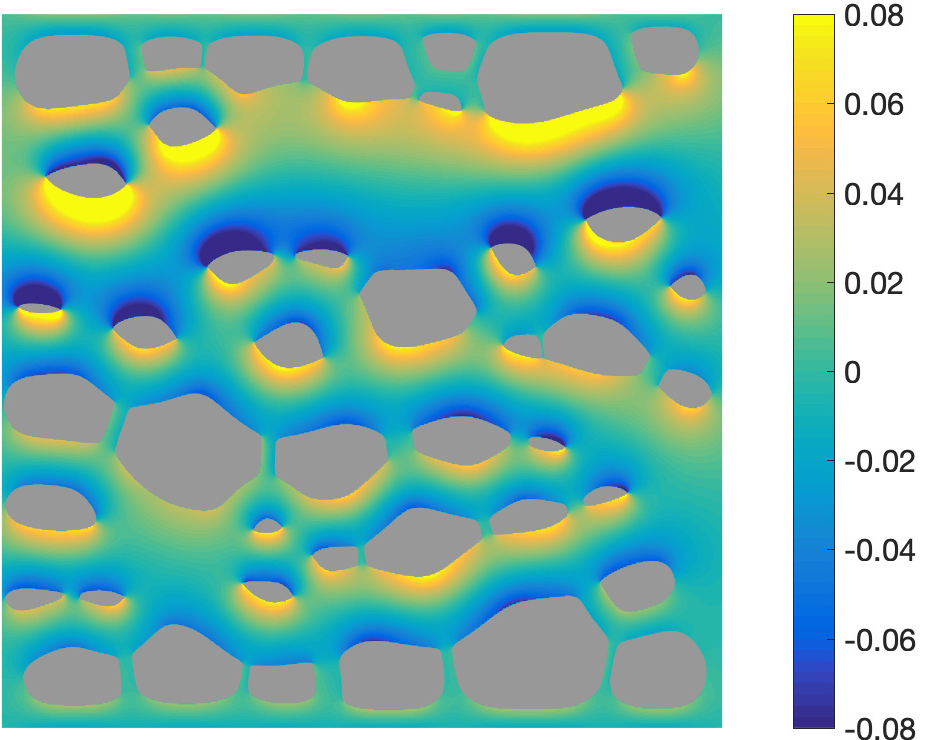
\includegraphics[width = 0.38 \textwidth]{./figs/vort_50b400}
\caption{\label{fig:Eroding50vort} Erosion of 50 nearly touching
bodies with the fixed pressure drop condition. The color is the
vorticity of the fluid. The 6 snapshots are evenly spaced in time.}
\end{center}
\end{figure}

%%%%%%%%%%%%%%%%%%%%%%%%%%%%%%%%%%%%%%%%%%%%%%%%%%%%%%%%%%%%%%%%%%%%%%%
\paragraph{Contributions}
Our first main contribution is extending the work of Barnett et
al.~\cite{bar-wu-vee2015} so that high-order accurate derivatives of
solutions of the Stokes equations can be computed.  Using this new
quadrature method, we can accurately compute erosion rates, and
therefore stably simulate erosion.  Moreover, we use the quadrature
method to visualize the vorticity in the fluid bulk.  The vorticity is
convenient to visualize since, in the zero Reynolds number limit, it is
equivalent to the shear stress on the eroding bodies, and therefore its
magnitude is the erosion rate.

Our second contribution is computing trajectories in the eroded
geometries.  These trajectories are used to characterize the transport
by computing local tortuosities of the trajectories, the tortuosity of
the eroded geometry, and the anomalous dispersion rates in the geometry.
Again, by using an appropriate quadrature method~\cite{bar-wu-vee2015},
and a fourth-order Runge-Kutta method, we are able to stably compute
trajectories that spend large amounts of time in the slow velocity
regions near the eroding bodies, and computing these trajectories
reliably is essential to characterize the flow.  We compare our
tortuosity and dispersion rates with models available in the literature.

%%%%%%%%%%%%%%%%%%%%%%%%%%%%%%%%%%%%%%%%%%%%%%%%%%%%%%%%%%%%%%%%%%%%%%%
\paragraph{Limitations}
As in our previous work~\cite{qua-moo2018}, this work considers
two-dimensional immobile bodies. However, this new work does not have a
limitation on the packing of the bodies. Compared to our previous work,
we are able to simulate much denser suspensions with a comparable number
of discretization points.  While we do investigate transport in this
work, we only consider passive particles that are undergoing only
advection. To model other physical processes, such as contaminant
transport, we plan to simulate a finite Peclet number
advection-diffusion equation in eroded geometries.


%%%%%%%%%%%%%%%%%%%%%%%%%%%%%%%%%%%%%%%%%%%%%%%%%%%%%%%%%%%%%%%%%%%%%%%
\paragraph{Outline of the Paper}
In Section~\ref{sec:formulation}, we briefly summarize the model that we
describe in detail in our previous work~\cite{qua-moo2018}.  In
Section~\ref{sec:DLP}, we recast all the governing equations as layer
potentials defined in both $\RR^2$ and in $\CC$.
Section~\ref{sec:method} describes the numerical methods, with special
attention paid to the new quadrature method to compute the shear stress
and vorticity.  Section~\ref{sec:transport} describes measures for
characterizing the geometry, transport, and dispersion.
Section~\ref{sec:results} presents numerical examples for a variety of
dense packings of bodies.  Finally, concluding remarks are made in
Section~\ref{sec:conclusions}.

%%%%%%%%%%%%%%%%%%%%%%%%%%%%%%%%%%%%%%%%%%%%%%%%%%%%%%%%%%%%%%%%%%%%%%%
\section{Governing Equations}
\label{sec:formulation}
%%%%%%%%%%%%%%%%%%%%%%%%%%%%%%%%%%%%%%%%%%%%%%%%%%%%%%%%%%%%%%%%%%%%%%%
We start by defining the main variables used to model erosion.  A more
detailed description is in our previous work~\cite{qua-moo2018}.  We
consider flows inside a confined geometry $\Omega$ that contains $M$
eroding bodies with boundary $\gamma_\ell$, $\ell = 1,\ldots,M$.  The
boundary of the bounding geometry is $\Gamma$, and the fluid domain is
bounded by $\bd \Omega = \Gamma \cup \gamma_1 \cup \cdots \cup
\gamma_M$.  On each eroding body, $\nn$ is the normal vector pointing
into the body, and $\ss$ is the unit tangent vector pointing in the
counterclockwise direction.  The normal vector on $\Gamma$ is the
outward unit normal.  Neglecting inertial forces, the governing
equations are
\begin{equation}
\label{eqn:erosionModel}
  \begin{split}
    \mu \Delta \uu = \grad p, &\hspace{20pt} \xx \in \Omega, \gap 
      &&\mbox{\em conservation of momentum}\\
    \grad \cdot \uu = 0, &\hspace{20pt} \xx \in \Omega, \gap 
      &&\mbox{\em conservation of mass} \\
    \uu = 0, &\hspace{20pt} \xx \in \gamma, \gap 
      &&\mbox{\em no slip on the bodies} \\
    \uu = \UU, &\hspace{20pt} \xx \in \Gamma, \gap 
      &&\mbox{\em outer wall velocity} \\
    \Vn = \CE \, \abs{\tau}, &\hspace{20pt} \xx \in \gamma,
      &&\mbox{\em erosion model}.
  \end{split}
\end{equation}
Here, $\uu$ is the fluid velocity, $p$ is the pressure, $\UU$ is a
prescribed Hagen-Poiseuille velocity field, $\Vn$ is the normal velocity
of $\gamma$, and
\begin{align}
  \tau = -(\nabla \uu + \nabla \uu^T) \nn \cdot \ss
  \label{eqn:shearStress}
\end{align}
is the shear stress on $\gamma$.

The erosion rate loses differentiability if the shear stress changes
sign, and this leads to corners developing on $\gamma$ and numerical
instabilities.  Therefore, we modify the erosion rate by adding a
curvature penalization. That is, the erosion model
in~\eqref{eqn:erosionModel} is replaced with 
\begin{align}
  \Vn = \CE \, \abs{\tau} + \epsilon \langle\abs{\tau}\rangle \left(
    \frac{L}{2\pi} \kappa - 1 \right),
\end{align}
where $\epsilon \ll 1,$ $\langle \cdot \rangle$ is the spatial average,
$L$ is the length of $\gamma$, and $\kappa$ is the curvature of
$\gamma$.  The normalization term guarantees that the regularization
only changes the body's shape, but not its total length.  Finally, to
increase the overall stability of the method, a narrow Gaussian filter
is applied to the erosion rate.

%%%%%%%%%%%%%%%%%%%%%%%%%%%%%%%%%%%%%%%%%%%%%%%%%%%%%%%%%%%%%%%%%%%%%%%
\section{Boundary Integral Equation Formulation}
\label{sec:DLP}
%%%%%%%%%%%%%%%%%%%%%%%%%%%%%%%%%%%%%%%%%%%%%%%%%%%%%%%%%%%%%%%%%%%%%%%
Applying the same approach as our previous work~\cite{qua-moo2018}, we
use a double-layer potential formulation for the velocity $\uu$.  The
double-layer potential is
\begin{align}
  \DDD[\eeta](\xx) = \int_{\bd\Omega} D(\xx,\yy) \eeta(\yy)\, ds_\yy = 
  \frac{1}{\pi}\int_{\bd\Omega} 
    \frac{\rr \cdot \nn}{\rho^2} \frac{\rr \otimes \rr}{\rho^2}
    \eeta(\yy) \, ds_\yy, \quad \xx \in \Omega,
  \label{eqn:velocityDLP}
\end{align}
where $D$ is the kernel of the integral operator, $\rr = \xx - \yy$,
$\rho = \|\rr\|$, $\nn$ is the unit outward normal at $\yy$, and $\eeta$
is an unknown density function.  Since the Stokes double-layer potential
can not represent all solutions of the incompressible Stokes equations,
we complete the integral equation formulation by adding the Stokeslets
and rotlets~\cite{pow-mir1987}
\begin{align}
  S[\llambda_\ell,\cc_\ell](\xx) = \frac{1}{4\pi} \left( 
    -\log \rho \II + \frac{\rr \otimes \rr}{\rho^2}
    \right)\llambda_\ell, \quad
  R[\xi_\ell,\cc_\ell](\xx) = \frac{\rr^\perp}{\rho^2} \xi_\ell,
\end{align}
where $\rr = \xx - \cc_\ell$, $\cc_\ell$ is a point inside the
$\ell^{th}$ eroding body, $\rr^\perp = (r_2,-r_1)$, and $\rho =
\|\rr\|$.  Then, for any sufficiently smooth geometry $\Omega$, the
solution of the incompressible Stokes equation with a Dirichlet boundary
condition $\ff$ is
\begin{align}
  \uu(\xx) = \DDD[\eeta](\xx) + 
    \sum_{\ell=1}^M S[\llambda_\ell,\cc_\ell](\xx) + 
    \sum_{\ell=1}^M R[\xi_\ell,\cc_\ell](\xx),
\end{align}
where the density function, Stokeslets, and rotlets satisfy
\begin{subequations}
\label{eqn:BIE}
\begin{align}
  \ff(\xx) &= -\frac{1}{2}\eeta(\xx) + \DDD[\eeta](\xx) + 
    \sum_{\ell=1}^M S[\llambda_\ell,\cc_\ell](\xx) + 
    \sum_{\ell=1}^M R[\xi_\ell,\cc_\ell](\xx) +
    \NN_0[\eeta](\xx), \quad \xx \in \bd\Omega, \\
  \llambda_\ell &= \frac{1}{2\pi} \int_{\gamma_\ell} 
    \eeta(\yy)\, ds_\yy \quad \ell = 1,\ldots,M, \\
  \xi_\ell &= \frac{1}{2\pi} \int_{\gamma_\ell}
    (\yy - \cc_\ell)^\perp \cdot \eeta(\yy)\, ds_\yy 
    \quad \ell = 1,\ldots,M.
\end{align}
\end{subequations}
The operator $\NN_0$ is the integral operator with kernel
$N_(0)(\xx,\yy) = \nn(\xx) \otimes \nn(\yy)$, $\xx,\yy \in \Gamma$,
which removes the rank one null space resulting from the flux-free
requirement of $\ff$.  In this work, $\ff$ is the prescribed velocity,
$\UU$, on the outer wall, $\Gamma$, and is zero on the eroding bodies,
$\gamma_\ell$, $\ell=1,\ldots,M$.  

The deformation tensor, pressure, and vorticity of the double-layer
potential, Stokeslets, and rotlets, can all be computed analytically in
terms of the density function and the strengths of the Stokeslets and
rotlets.  For $\xx \in \Omega$, the deformation tensor, pressure, and
vorticity of the double-layer potential~\eqref{eqn:velocityDLP} are
\begin{align}
  \label{eqn:deformationDLP} 
  \ssigma(\xx) &= \int_{\bd\Omega} \mathbf{D}_{\ssigma}(\xx,\yy) 
      \eeta(\yy) ds_{\yy} 
  = \frac{1}{2\pi}\int_{\bd\Omega} \left(
    2\frac{\rr \cdot \nn}{\rho^2} \frac{\rr \cdot \eeta}{\rho^2} \II + 
    \frac{\rr \cdot \eeta}{\rho^4} (\nn \otimes \rr + \rr \otimes \nn) 
    \right. \nonumber \\
    & \qquad\qquad\qquad\qquad\qquad\qquad \left.
    +\frac{\rr \cdot \nn}{\rho^4} (\eeta \otimes \rr + \rr \otimes \eeta) - 
    8\frac{(\rr \cdot \nn)(\rr \cdot \eeta)}{\rho^6}(\rr \otimes \rr)
    \right) \, ds_\yy, \\
%
  p(\xx) &= \int_{\bd\Omega} D_{p}(\xx,\yy) 
      \eeta(\yy) ds_{\yy} 
  = -\frac{1}{\pi}\int_{\bd\Omega} \frac{1}{\rho^2}
    \left(I - 2 \frac{\rr \otimes \rr}{\rho^2}\right) \nn \cdot
      \eeta(\yy)\,ds_\yy, \\
%
  \label{eqn:vorticityDLP} 
  \omega(\xx) &= \int_{\bd\Omega} D_{\omega}(\xx,\yy) 
      \eeta(\yy) ds_{\yy} 
  = -\frac{1}{\pi} \int_{\bd\Omega}
    \frac{(\rr \cdot \nn^\perp) + (\rr \cdot \nn)}{\rho^4} 
      (\rr \cdot \eeta) \, ds_\yy,
\end{align}
respectively. We require the deformation tensor of the double-layer potential at
$\xx \in \bd \Omega$.  Since the deformation tensor of the double-layer
potential is discontinuous across $\bd\Omega$, the jump term 
\begin{align}
  \frac{1}{2} \left(\pderiv{\eeta}{\ss} \cdot \ss \right) \left[
    \begin{array}{cc}
      s_x^2 - s_y^2 & 2s_x s_y \\ 2s_x s_y & s_y^2 - s_x^2
    \end{array}
  \right],
  \label{eqn:deformationJump}
\end{align}
must be added to $\ssigma(\xx)$ for $\xx \in \bd\Omega$.  Finally, the
Stokeslets and rotlets do not have any jumps on $\gamma$, so the
deformation tensor, pressure, and vorticity due to the Stokeslets and
rotlets are straightforward to compute~\cite{poz1992} \todo[inline]{BQ:
Make sure this is the right reference}.  Having computed the deformation
tensor on $\gamma$, the shear stress is computed as defined in
equation~\eqref{eqn:shearStress}.  

%%%%%%%%%%%%%%%%%%%%%%%%%%%%%%%%%%%%%%%%%%%%%%%%%%%%%%%%%%%%%%%%%%%%%%%
\subsection{Cauchy Integral Representation of the Double-Layer
Potential}
\label{sec:DLPcomplex}
%%%%%%%%%%%%%%%%%%%%%%%%%%%%%%%%%%%%%%%%%%%%%%%%%%%%%%%%%%%%%%%%%%%%%%%
In equations~\eqref{eqn:velocityDLP} and~\eqref{eqn:deformationDLP},
$\uu$ and its deformation tensor are written as a contour integral in
$\RR^2$.  However, so that we can apply a particular quadrature method,
we need to write these layer potentials in terms of Cauchy integrals in
$\CC$ and their derivatives.  The first step is to write the Laplace
double-layer potential as the complex integral
\begin{align}
  \DD[\eta](\xx) = \frac{1}{2\pi} \int_{\bd\Omega} 
    \frac{\rr \cdot \nn}{\rho^2}\, ds_\yy = \Re (v(x)) \quad 
    \text{where} \quad v(x) = \frac{1}{2\pi i} \int_{\bd\Omega}
    \frac{\eta(y)}{x - y} \, dy,
  \label{eqn:laplaceComplex}
\end{align}
where $\xx,\yy \in \RR^2$ are identified with the points $x,y \in \CC$.
Equation~\eqref{eqn:laplaceComplex} can be converted to a Cauchy
integral by first finding the boundary data of $v$.  We assume that
$\Omega$ is a simply-connected interior domain. Then, the boundary data
of $v$ satisfies the Sokhotski-Plemelj jump relation
\begin{align}
  \label{eqn:SPrelation}
  v(x) = - \frac{1}{2} \eta(x) + \frac{1}{2\pi i} \int_{\bd\Omega}
    \frac{\eta(y)}{x-y}\, dy, \quad x \in \bd\Omega.
\end{align}
For exterior domains, the jump term changes from $-1/2$ to $1/2$, and
for multiply-connected domains, such as a porous media, $\bd\Omega$ is
simply decomposed into its different connected components and the
appropriate Cauchy integral is evaluated.  Since $v$ is a holomorphic
function and we have its boundary data, by the Cauchy integral theorem
we have
\begin{align}
  \label{eqn:cauchy}
  v(x) = \frac{1}{2\pi i}\int_{\bd\Omega} 
    \frac{v(y)}{y-x} \,dy, \quad
  v'(x) = \frac{1}{2\pi i} \int_{\bd\Omega}
    \frac{v(y)}{(y-x)^2} \, dy, \quad
  v''(x) = \frac{1}{\pi i} \int_{\bd\Omega}
    \frac{v(y)}{(y-x)^3} \, dy,
\end{align}
for $x \in \Omega$.  Since $v(x)$ depends on the density function $\eta
\in \CC$, we use the notation $v[\eta](x)$ to denote the holomorphic
function defined in equation~\eqref{eqn:laplaceComplex}, and its first
two derivatives are written as $v'[\eta](x)$ and $v''[\eta](x)$.  
  
To rewrite the Stokes double-layer potential~\eqref{eqn:velocityDLP} in
terms of Cauchy integrals and their derivatives, we write it in terms of
Laplace layer potentials
\begin{equation}
  \label{eqn:Stokes2Laplace}
  \begin{aligned}
    \DDD[\eeta](\xx) &= 
      \frac{1}{2\pi} \int_{\bd\Omega} 
        \frac{\nn}{\rho^2} (\rr \cdot \eeta) \, ds_\yy + 
      \frac{1}{2\pi} \nabla \int_{\bd\Omega}
        \frac{\rr \cdot \nn}{\rho^2} (\yy \cdot \eeta) \, ds_\yy \\
      &- \frac{1}{2\pi} x_1 \nabla \int_{\bd\Omega}
        \frac{\rr \cdot \nn}{\rho^2}\eta_1(\yy) \, ds_\yy -
      \frac{1}{2\pi} x_2 \nabla \int_{\bd\Omega}
        \frac{\rr \cdot \nn}{\rho^2}\eta_2(\yy) \, ds_\yy.
  \end{aligned}
\end{equation}
Therefore, the Stokes double-layer potential can be written in terms of
Cauchy integrals and their first derivative  as~\cite{bar-wu-vee2015}
\begin{equation}
  \begin{aligned}
    u_1(x) &= \Re (v[\tau_1](x)) + \Re (v'[y\cdot\eta](x)) 
             -x_1\Re (v'[\eta_1](x)) - x_2\Re (v'[\eta_2](x)), \\
    u_2(x) &= \Re (v[\tau_2](x)) - \Im (v'[y\cdot\eta](x)) 
         +x_1\Im (v'[\eta_1](x)) + x_2\Im (v'[\eta_2](x)),
  \end{aligned}
  \label{eqn:cauchyVelocity}
\end{equation}
where $y \cdot \eta = y_1 \eta_1 + i y_2 \eta_2 \in \CC$, 
\begin{align} 
  \tau_1=(\eta_1+i\eta_2)\frac{\Re(n)}{n}, \quad
  \tau_2=(\eta_1+i\eta_2)\frac{\Im(n)}{n},
\end{align}
and $n \in \CC$ is the complex representation of the outward unit normal
$\nn \in \RR^2$.


%%%%%%%%%%%%%%%%%%%%%%%%%%%%%%%%%%%%%%%%%%%%%%%%%%%%%%%%%%%%%%%%%%%%%%%
\subsection{Cauchy Integral Representation for the Gradient of the
Double-Layer Potential}
\label{sec:gradDLPcomplex}
%%%%%%%%%%%%%%%%%%%%%%%%%%%%%%%%%%%%%%%%%%%%%%%%%%%%%%%%%%%%%%%%%%%%%%%
In addition to the velocity, we require a complex-valued representation
of the gradient of the velocity so that we can compute the shear stress
and the vorticity.  The deformation tensor at $x \in \Omega$ is found by
computing the derivatives of $u_1$ and $u_2$ as defined in
equation~\eqref{eqn:cauchyVelocity}  
\begin{equation}
\label{eqn:cauchyGradient}
  \begin{aligned}
    \pderiv{u_1}{x_1} &= +\Re (v'[\tau_1](x)) + 
      \Re (v''[y\cdot\eta](x)) - \Re (v'[\eta_1](x)) - 
      x_1\Re (v''[\eta_1](x)) - x_2\Re (v''[\eta_2](x)), \\
    \pderiv{u_1}{x_2} &= - \Im (v'[\tau_1](x)) - 
      \Im (v''[y\cdot\eta](x)) + x_1\Im (v''[\eta_1](x)) - 
      \Re (v'[\eta_2](x)) + x_2\Im (v''[\eta_2](x)), \\
    \pderiv{u_2}{x_1} &= +\Re (v'[\tau_2](x)) - 
      \Im (v''[y\cdot\eta](x)) + \Im (v'[\eta_1](x)) +
      x_1\Im (v''[\eta_1](x)) + x_2\Im (v''[\eta_2](x)), \\
    \pderiv{u_2}{x_2} &= -\Im (v'[\tau_2](x)) - 
      \Re (v''[y\cdot\eta](x)) + x_1\Re (v''[\eta_1](x)) +
      \Im (v'[\eta_2](x)) + x_2\Re (v''[\eta_2](x)).
  \end{aligned}
\end{equation}
The same expressions are used to compute the deformation tensor for $x
\in \bd\Omega$, except that the jump
condition~\eqref{eqn:deformationJump} is included.  Finally, to compute
the shear stress, the deformation tensor on $\bd\Omega$ is applied to
the normal and tangent vectors as defined in
equation~\eqref{eqn:shearStress}.

In a shear flow, the vorticity is equivalent to the shear stress.  Since
the erosion rate is proportional to the magnitude of the shear stress,
it is constructive to visualize the vorticity of the fluid.  For $x \in
\Omega$, the Cauchy integral representation of the vorticity is
\begin{align}
  \omega(x) = \pderiv{u_2}{x_1} - \pderiv{u_1}{x_2} = 
\Re (v'[\tau_2](x)) + \Im (v'[\tau_1](x)) 
 + \Re (v'[\eta_2](x))+ \Im (v'[\eta_1](x)), \quad x \in \Omega.
\end{align}


%%%%%%%%%%%%%%%%%%%%%%%%%%%%%%%%%%%%%%%%%%%%%%%%%%%%%%%%%%%%%%%%%%%%%%%
\section{Transport, Tracers, and Tortuosity}
\label{sec:transport}
%%%%%%%%%%%%%%%%%%%%%%%%%%%%%%%%%%%%%%%%%%%%%%%%%%%%%%%%%%%%%%%%%%%%%%%
Erosion leads to interesting porous geometries, and we are interested in
characterizing transport in these geometries.  In our previous
work~\cite{qua-moo2018}, we examined the effect of erosion on the area
fraction, flow rate, and the total drag.  However, to characerize
transport, other quantities must be examined.  Here, we compute the
anomalous dispersion rate, the tortuosity, and the distribution of the
gap sizes.  The first two metrics can be defined in terms of streamline
governed by an advection autonomous equation~\eqref{eqn:tracers}.

%%%%%%%%%%%%%%%%%%%%%%%%%%%%%%%%%%%%%%%%%%%%%%%%%%%%%%%%%%%%%%%%%%%%%%%
\subsection{Anomalous Disperision}
\label{sec:dispersion}
%%%%%%%%%%%%%%%%%%%%%%%%%%%%%%%%%%%%%%%%%%%%%%%%%%%%%%%%%%%%%%%%%%%%%%%
The dynamics of fluid in porous media is often characterized in terms of
anomalous dispersion~\cite{kla-rad-sok2008, den-cor-sch-ber2004}.  The
anomalous dispersion rate depends on the porosity and
permeability~\cite{koc-bra1988}, but the distribution of the bodies also
affects the anomalous dispersion rates.  Since erosion causes certain
structure in porous media, calculating the anomalous dispersion rates in
these geometries is important.

We calculate the anomalous dispersion rates by analyzing the streamlines
governed by equation~\eqref{eqn:tracers} for geometries that are formed
by erosion.  Given a set of trajectories, we define $\lambda_j(t)$ to be
the arclength of the trajectory
\begin{align}
  \lambda_j(t) = \int_{0}^t \|\ss'_j(\tau)\|\, d\tau, 
    \quad j=1,\ldots,N_p.
\end{align}
Then, the first and second ensemble moments are
\begin{align}
  \label{eqn:moments}
  \langle \lambda \rangle (t) = 
    \frac{1}{N_p} \sum_{j=1}^{N_p} \lambda_j(t), \quad 
    \sigma_\lambda^2(t) = \frac{1}{N_p} 
    \left[\lambda_j(t) - \langle \lambda \rangle(t) \right]^2.
\end{align}
Since we compute second-order statistics, we use 1000 streamlines so
that the statistics have converged~\cite{bel-sal-rin1992}.  Then,
particle dispersion is characterized as $\sigma_\lambda$.  At early
times, the particles have not explored much of the geometry, and we
expect a ballistic motion $\sigma_\lambda \sim t$.  However, as the
particles pass the grains, their trajectories are altered, and we expect
that $\sigma_\lambda \sim t^\alpha$, with $\alpha \in (0.5,1)$,
indicating that the flow is super-dispersive.

To establish an anomalous dispersion rate, the trajectories must pass
several grains so that an asymptotic regime is reached. The geometries
that we consider are too short to observe the asymptotic dispersion, so
we use a reinsertion method to form longer trajectories. Similar to the
work of others~\cite{dea-qua-bir-jua2018, puy-gou-den2019}, once a
particle reaches the end of the porous region, it is reinserted at the
start of the porous region.  To minimize errors caused by the
reinsertion, the particle is initialized at the discretization point
that has the closest velocity to the particles velocity at the outlet.
After a single trajectory is formed, it has undergone a collection of
reinsertions.  The fore, as a post-processing step, the trajectory is made
continuous by attaching the tail of each segment to the origin of the
next segment.  

We consider trajectories in an open channel so that they can be compared
to trajectories in eroded geometries with large permeability.  The
trajectory originating at $(s_1(0),s_2(0))$ is
\begin{align}
  s_1(t) = (1-s_2(0)^2)t + s_1(0), \quad
  s_2(t) = s_2(0).
\end{align}
Averaging over $s_2(0) \in [-1,1]$, the first and second ensemble
moments are
\begin{align}
  \langle \lambda \rangle (t) = \frac{2}{3}t, \quad 
    \sigma_\lambda^2(t) = \frac{4}{45}t^2,
\end{align}
so the particle motion is ballistic since $\sigma_\lambda \sim t$.  In
Section~\ref{sec:results}, we compare these moments in an open channel
with the trajectories in an eroded geometry.


%%%%%%%%%%%%%%%%%%%%%%%%%%%%%%%%%%%%%%%%%%%%%%%%%%%%%%%%%%%%%%%%%%%%%%%
\subsection{Tortuosity}
%%%%%%%%%%%%%%%%%%%%%%%%%%%%%%%%%%%%%%%%%%%%%%%%%%%%%%%%%%%%%%%%%%%%%%%
The tortuosity of a geometry, denoted by $T \geq 1$, is a dimensionless
number that quantifies the average amount of turning made by
trajectories passing through the geometry.  Unlike the for the
dispersion, we do not use reinsertion to form long trajectories.  The
local tortuosity
\begin{align}
  \tau(y) = \frac{\lambda(y)}{d},
  \label{eqn:localTort}
\end{align}
is the length of a single trajectory, $\lambda(y)$, whose initial
$y$-coordinate is a value $y$ on a cross-section of length $d$.  Taking
the average over all points on the cross-section defines the hydraulic
tortuosity
\begin{align}
  T = \frac{1}{d}\frac{\displaystyle\int_{S}u_x(y)\lambda(y)\,dy}
  {\displaystyle\int_{S}u_x(y)\,dy},
  \label{eqn:tortuosity1}
\end{align}
where $S$ is a cross-section perpendicular to the $x$-axis with length
$d$, $\lambda(y)$ is the length of the trajectory that is initialized at
the $y$-coordinate along $S$, and $u_x(y)$ is the $x$ component of the
velocity at the $y$-coordinate along $S$.  Therefore, the tortuosity
satisfies $T \geq 1$, and $T=1$ only if no grains are present.  

The choice for the trajectory with length $\lambda(y)$ is not universal,
and Duda et al.~\cite{dud-koz-mat2011} summarize several options. One
choice, which we adopt, considers trajectories that originate at $S$ and
terminate at a parallel cross-section.  We use the cross-sections $x=-1$
and $x=1$.  This choice of averaging allows us to also compute the
tortuosity in terms of an area integral.  Under the assumptions that the
flow is incompressible and not re-entrant, meaning that all streamlines
connect the two cross-sections, the tortuosity in
equation~\eqref{eqn:tortuosity1} is equivalent to~\cite{dud-koz-mat2011}
\begin{align}
  T = \frac{\displaystyle\int_\Omega \|\uu(\yy)\|\, d\yy}
           {\displaystyle\int_\Omega u_x(\yy)\, d\yy},
  \label{eqn:tortuosity2}
\end{align}
where $\Omega$ is the fluid region between the inlet and outlet
cross-sections.  Recirculation zones are possible in viscous
fluids~\cite{hig1985}, but they are very small in the examples we
consider and have a negligible effect on the tortuosity.  Since
equation~\eqref{eqn:tortuosity2} does not require the additional work of
computing particle trajectories at every time step, we use this
definition for the majority of the tortuosity calculations.  However, we
do compare the two formulas for the tortuosity at several time steps in
Section~\ref{sec:results}.

There have been efforts to relate the tortuosity to the porosity.  For
example, Matyka et al.~\cite{mat-kha-koz2008} propose the models
\begin{subequations}
  \label{eqn:tortuosityModels}
  \begin{align}
    \widehat{T}(\phi) &= \phi^{-p}, \\
    \widehat{T}(\phi) &= 1-p \log \phi, \\
    \widehat{T}(\phi) &= 1+p (1-\phi), \\
    \widehat{T}(\phi) &= (1+p (1-\phi))^2, 
  \end{align}
\end{subequations}
where $p>0$ is a fitting parameter.  In Section~\ref{sec:results}, we
compare these four models with the tortuosity of eroding geometries.

%%%%%%%%%%%%%%%%%%%%%%%%%%%%%%%%%%%%%%%%%%%%%%%%%%%%%%%%%%%%%%%%%%%%%%%
\subsection{Pore Throat Size}
%%%%%%%%%%%%%%%%%%%%%%%%%%%%%%%%%%%%%%%%%%%%%%%%%%%%%%%%%%%%%%%%%%%%%%%
\begin{itemize}
  \item Pore throat sizes affect many things such as first passage time,
  mixing, chemical reactions, heat conduction, biological activities
\end{itemize}



%%%%%%%%%%%%%%%%%%%%%%%%%%%%%%%%%%%%%%%%%%%%%%%%%%%%%%%%%%%%%%%%%%%%%%%
\section{Numerical Methods}
\label{sec:method}
%%%%%%%%%%%%%%%%%%%%%%%%%%%%%%%%%%%%%%%%%%%%%%%%%%%%%%%%%%%%%%%%%%%%%%%
In line with our previous work~\cite{qua-moo2018}, we use two meshes to
simulate erosion. The integral equation is solved by discretizing the
boundary of the geometry at a set of points distributed equally in
arclength, and then applying a collocation method
(Section~\ref{sec:spatialDiscretization}).  The quadrature rule is
either the trapezoid rule or the Barycentric quadrature rule
(Section~\ref{sec:bary}).  The selection algorithm that determines which
quadrature method is applied is described in Section~\ref{sec:fmm}.
Once the shear stress is computed, the bodies are eroded a single time
step by using a {\thL} discretization~\cite{hou-low-she1994}.  By using
a {\thL} formulation, the stiff curvature term is linear and the
discretization points remain equispaced in arclength.  Finally, time
stepping methods for the eroding bodies and passive particles are
described in Section~\ref{sec:time}

%%%%%%%%%%%%%%%%%%%%%%%%%%%%%%%%%%%%%%%%%%%%%%%%%%%%%%%%%%%%%%%%%%%%%%%
\subsection{Spatial Discretization}
\label{sec:spatialDiscretization}
%%%%%%%%%%%%%%%%%%%%%%%%%%%%%%%%%%%%%%%%%%%%%%%%%%%%%%%%%%%%%%%%%%%%%%%
By using an integral equation formulation, we only have to discretize
the one-dimensional boundary of the domain.  Therefore, we easily
resolve complex geometries, and differentiation is performed with
spectral accuracy in Fourier space.  We discretize each eroding body
$\gamma_k$ with $N_\iin$ points and discretize the outer wall $\Gamma$
with $N_\out$ points.  The $j^{th}$ discretization point on $\Gamma$ and
$\gamma_k$ are denoted by $\yy_j^0$ and $\yy^k_j$, respectively.  The
discretization points are initially distributed evenly in arclength, and
this equispacing is maintained for the entire simulation by using the
{\thL} formulation.  In addition, we apply mild smoothing
strategies~\cite{qua-moo2018} to avoid the corners that erosion
inevitably develop.

Given the discretization points of $\bd\Omega$, applying the trapezoid
rule results in the collocation method for~\eqref{eqn:BIE} 
\begin{subequations}
\label{eqn:trapLinearSystem}
  \begin{alignat}{3}
  \UU_\ell &= \sum_{j=1}^{N_\out} 
    w^0_j D(\yy^0_\ell,\yy^0_j) \eeta_j +
  \sum_{k=1}^M \sum_{j=1}^{N_\iin}
    w^k_j D(\yy^0_\ell,\yy^k_j) \eeta^k_j +
  \sum_{j=1}^{N_\out} w^0_j N_0(\yy^0_\ell,\yy^0_j) \nonumber \\
  &\quad+\sum_{k=1}^M S[\llambda_k,\cc_k](\yy^0_\ell) + 
  \sum_{k=1}^M R[\xi_k,\cc_k](\yy^0_\ell),
    &&\hspace{-60pt} \ell = 1,\ldots,N_\out, \\
%
  \mathbf{0} &= \sum_{j=1}^{N_\out} 
    w^0_j D(\yy^m_\ell,\yy^0_j) \eeta_j +
  \sum_{k=1}^M \sum_{j=1}^{N_\iin}
    w^k_j D(\yy^m_\ell,\yy^k_j) \eeta^k_j \nonumber \\
  &\quad+\sum_{k=1}^M S[\llambda_k,\cc_k](\yy^m_\ell) + 
  \sum_{k=1}^M R[\xi_k,\cc_k](\yy^m_\ell),
    &&\hspace{-60pt}\ell = 1,\ldots,N_\iin, \: m=1,\ldots,M, \\
%
  \llambda_m &= \frac{1}{2\pi} \sum_{j=1}^{N_\iin} \eeta^m_j,  \quad
  \xi_m = \frac{1}{2\pi} \sum_{j=1}^{N_\iin}
    (\yy^m_j - \cc_m)^\perp \cdot \eeta^m_j,
    &&\hspace{-60pt} m=1,\ldots,M,
\end{alignat}
\end{subequations}
where $w^k_j$ are quadrature weights (which depend on $N_\iin$,
$N_\out$, and the lengths of $\gamma^k$), and $D$ is the kernel of the
Stokes double-layer potential defined in
Equation~\eqref{eqn:velocityDLP}.  The linear
system~\eqref{eqn:trapLinearSystem} is a well-conditioned second-kind
integral equation that is solved iteratively with GMRES.  If the number
of discretization points is sufficiently large, then the solution
of~\eqref{eqn:trapLinearSystem} is an accurate approximation of the
density function, Stokeslets, and rotlets.   Then, if $\xx \in \Omega$
is sufficiently far from $\bd\Omega$, an approximation of the velocity,
deformation tensor, and vorticity due to the double-layer potential is
found by applying the trapezoid rule to \eqref{eqn:velocityDLP},
\eqref{eqn:deformationDLP}, and~\eqref{eqn:vorticityDLP}, respectively.
In particular,
\begin{align}
  \label{eqn:trap}
  \uu(\xx) &= \sum_{j=1}^{N_\out} w^0_j D(\xx,\yy^0_j) \eeta_j +
  \sum_{k=1}^M \sum_{j=1}^{N_\iin} w^k_j D(\xx,\yy^k_j) \eeta^k_j, \\
%
  \ssigma(\xx) &= \sum_{j=1}^{N_\out} w^0_j \mathbf{D}_\ssigma(\xx,\yy^0_j) \eeta_j +
  \sum_{k=1}^M \sum_{j=1}^{N_\iin} w^k_j \mathbf{D}_\ssigma(\xx,\yy^k_j)
  \eeta^k_j, \\
%
  w(\xx) &= \sum_{j=1}^{N_\out} w^0_j D_\omega(\xx,\yy^0_j) \eeta_j +
  \sum_{k=1}^M \sum_{j=1}^{N_\iin} w^k_j D_\omega(\xx,\yy^k_j)
  \eeta^k_j.
\end{align}
The contributions due to the Stokeslets and rotlets require no
quadrature and are easily included in the velocity, deformation tensor,
and vorticity.  Finally, to compute the shear stress, we apply the
trapezoid rule with Fourier differentiation to approximate the jump
term~\eqref{eqn:deformationJump} of the deformation tensor, and then the
tensor is applied to the normal and tangent vectors as defined in
equation~\eqref{eqn:shearStress}.

Once the velocity is computed in $\Omega$, the tortuosity can be
computed with the Eulerian velocity field~\eqref{eqn:tortuosity2}.  We
first compute the velocity at $\xx_{ij} = (-1 + i\Delta x, -1 + j\Delta
y)$, $i,j=1,\ldots,N$, where $\Delta x = \Delta y = 2/N$, and the
velocity at points inside an eroding body are assigned a value of 0.
Then, the tortuosity is approximated as
\begin{align}
  T = \frac{\sum\limits_{i,j=1}^N \|\uu(\xx_{ij})\|\Delta x \Delta y}
      {\sum\limits_{i,j=1}^N u_x(\xx_{ij}) \Delta x \Delta y}.
\end{align}

%%%%%%%%%%%%%%%%%%%%%%%%%%%%%%%%%%%%%%%%%%%%%%%%%%%%%%%%%%%%%%%%%%%%%%%%
\subsection{Barycentric Quadrature Formulas}
\label{sec:bary}
%%%%%%%%%%%%%%%%%%%%%%%%%%%%%%%%%%%%%%%%%%%%%%%%%%%%%%%%%%%%%%%%%%%%%%%
Since the error of the trapezoid rule applied to periodic functions
depends on the derivative of the integrand~\cite{tre-wei2014}, the
trapezoid rule applied in Section~\ref{sec:spatialDiscretization} is
only appropriate if the target point is sufficiently separated from all
eroding bodies and the outer wall.  Therefore, if the trapezoid rule is
applied when bodies are in near-contact, or when a layer potential is
evaluated at a point close to $\bd\Omega$, then the results become
unreliable and ultimately unusable.  Hence, we require a quadrature
method whose error is bounded independent of the target location.

We showed in Sections~\ref{sec:DLPcomplex} and
Section~\ref{sec:gradDLPcomplex} that the velocity, shear stress, and
vorticity of the double-layer representation can all be written in terms
of Cauchy integrals and its first two derivatives.  Therefore, if we
develop quadrature rules with a uniformly bounded error for Cauchy
integrals and its derivatives~\eqref{eqn:cauchy}, then the quadrature
method can be used to accurately compute the velocity, shear stress, and
vorticity.  Ioakimidis et al.~\cite{ioa-pap-per1991} developed
quadrature methods, that we call {\em Barycentric quadrature rules}, to
compute Cauchy integrals and their derivatives with an error bound that
is independent of $x$.  Then, Barnett et al.~\cite{bar-wu-vee2015}
applied these quadrature methods to compute the Stokes double-layer
potential representation of the velocity~\eqref{eqn:velocityDLP}.  We
build on this method so that the shear stress and vorticity can be
computed with a uniform error bound.

We briefly summarize the Baryncentric quadrature method for computing
the velocity~\cite{bar-wu-vee2015}.  Then, so that we can simulate and
visualize erosion, we apply similar techniques to compute Barycentric
quadrature rules for the gradient of the velocity.  We present the
quadrature for a simply-connected interior domain $\Omega$, and we
consider the target points $x \in \Omega$ and $x \in \Omega^c$. Then,
the method naturally extends to the eroding geometry by applying the
quadrature to each of its connected component.  The method starts with
an underlying quadrature rule, and we use the spectrally accurate
trapezoid rule.  Since the quadrature points are uniformly distributed,
the quadrature weights are $w_j = L/N$, $j=1,\ldots,N$, where $L$ is the
length of $\bd\Omega$.

Again, given a density function $\eta$, the boundary data of
$v[\eta](\xx)$, as defined in equation~\eqref{eqn:laplaceComplex},
satisfies the Sokhotski-Plemelj jump relation~\eqref{eqn:SPrelation}.
Since the boundary data of $v$ differs when considering $x \in \Omega$
and $x \in \Omega^c$, we denote the boundary data as $v^-$ for $x \in
\Omega$, and as $v^+$ otherwise.  Rather than directly applying the
trapezoid rule to $v(x)$, we start with the identity
\begin{align}
  \int_{\bd\Omega} \frac{v^{-}(y) - v(x)}{y - x} \,dy = 0,
    \quad x \in \Omega,
\end{align}
where we are considering the interior problem.  Since the integrand is
bounded as $x$ approaches $\bd\Omega$, we can apply the trapezoid rule
\begin{align}
  \sum_{j=1}^{N} \frac{v^{-}(y_j) - v(x)}{y_j - x} w_j \approx 0,
\end{align}
and the error is independent of $x$.  Rearranging for $v(x)$, we have
the interior Barycentric quadrature rule
\begin{align}
  v(x) = \frac{\sum\limits_{j=1}^N \frac{v^{-}(y_j)}{y_j - x} w_j}
  {\sum\limits_{j=1}^N \frac{1}{y_j - x} w_j}, \quad x \in \Omega.
  \label{eqn:BaryvInterior}
\end{align}
Using a similar construction and letting $a$ be any point inside
$\Omega$, the exterior Barycentric quadrature rule is
\begin{align}
  v(x) = \frac{1}{x-a} 
    \frac{\sum\limits_{j=1}^N \frac{v^+(y_j)}{y_j - x}w_j}
    {\sum\limits_{j=1}^N \frac{(y_j - a)^{-1}}{y_j - x}w_j},
    \quad x \in \Omega^c.
  \label{eqn:BaryvExterior}
\end{align}

Similar constructions can be used to derive quadrature rules
for $v'(x)$.  For $x \in \Omega$, we have the identity
\begin{align}
  \int_{\bd\Omega} \frac{v^-(y) - v(x) + (y-x)v'(x)}{(y - x)^2} = 0,
\end{align}
and the integrand is bounded for all $x \in \Omega$.  Therefore, after
applying the trapezoid rule and rearranging for $v'(x)$, we have the
interior Barycentric quadrature rule
\begin{align}
  v'(x) = \frac{\sum\limits_{j=1}^{N}
    \frac{v^{-}(y_j) - v(x)}{(y_j-x)^2} w_j}
  {\sum\limits_{j=1}^{N} \frac{1}{y_j-x} w_j}, 
  \quad x \in \Omega.
  \label{eqn:BaryvprimeInterior}
\end{align}
Using a similar construction, the exterior Barycentric quadrature rule
for the the first derivative is
\begin{align}
  v'(x) = \frac{1}{x-a} \frac{\sum\limits_{j=1}^N
    \frac{v^+_j - v(x)}{(y_j - x)^2} w_j}
    {\sum\limits_{j=1}^N \frac{(y_j-a)^{-1}}{y_j - x} w_j},
    \quad x \in \Omega^c.
  \label{eqn:BaryvprimeExterior}
\end{align}
Note that the value $v(x)$ is required to compute $v'(x)$ for both the
interior and exterior case, and these are available using the quadrature
rules~\eqref{eqn:BaryvInterior} and~\eqref{eqn:BaryvExterior}.

To compute the shear stress and vorticity, we require a Barycentric
quadrature rule for $v''(x)$.  The derivation is largely based on the
work of Ioakimidis et al.~\cite{ioa-pap-per1991} (see equation (2.12)).
We start with the second derivative of the Cauchy integral theorem
\begin{align}
  0 = \frac{1}{2\pi i} \int_{\bd\Omega} 
      \frac{2v^{-}(y)}{(y-x)^3}\,dy - v''(x).
\end{align}
For the interior case, $x \in \Omega$, we use the identity
\begin{align}
  \frac{1}{2\pi i}\int_{\bd\Omega} \frac{1}{(y-x)^n}\, dy = 
  \left\{
    \begin{array}{ll}
      1, & n = 1, \\
      0, & n = 2,3,\ldots. \\
    \end{array}
  \right.
\end{align}
Combining this identity with the Cauchy integral representation of
$v''(x)$, we have
\begin{align}
  0 = \frac{1}{2\pi i} \int_{\bd\Omega} 
      \frac{2v^{-}(y) - v''(x)(y-x)^2 - 2v(x) - 2(y-x)v'(x)}
      {(y-x)^3}\, dy.
\end{align}
This integrand is constructed so that it is bounded for all $x \in
\Omega$, and applying the trapezoid rule, we have
\begin{align}
  0 \approx  \sum_{j=1}^{N} 
      \frac{2v^{-}(y_j) - v''(x)(y_j-x)^2 - 2v(x) - 2(y_j-x)v'(x)}
      {(y_j-x)^3} w_j,
\end{align}
where the accuracy is independent of $x$.  Solving for $v''(x)$, the
Barycentric quadrature rule for the interior second derivative is
\begin{align}
  v''(x) &\approx \frac{2\sum\limits_{j=1}^N 
    \frac{v^{-}_{j} - v(x) - (y_j-x)v'(x)}{(y_j-x)^3}w_j}
    {\sum\limits_{j=1}^N \frac{1}{y_j-x}w_j}, \quad x \in \Omega.
\end{align}
For the exterior case, $x \in \Omega^c$, we start with the identity
\begin{align}
\frac{1}{x-a} &= -\frac{1}{2\pi i}\int_{\bd\Omega} 
    \frac{(y-a)^{-1}}{y-x}\, dy. 
\end{align}
Combining this identity with the Cauchy integral representation of
$v''(x)$, we have
\begin{align}
  0 = \frac{1}{2\pi i} \int_{\bd\Omega} 
    \frac{2v^+(y) - 2v(x) - 2(y-x)v'(x) + (y-a)^{-1} (x-a) (y-x)^2 v''(x)}
    {(y-x)^3}.
\end{align}
As in the interior case, the integrand is chosen so that it is bounded
for all $x \in \Omega^c$.  Therefore, after applying the trapezoid rule
and solving for $v''(x)$, we have the Barycentric quadrature rule for
the exterior second derivative
\begin{align}
  v''(x) &\approx \frac{1}{x-a}\frac{2\sum\limits_{j=1}^N
    \frac{v^{+}_{j} - v(x) - (y_j-x)v'(x)}{(y_j-x)^3}w_j}
    {\sum\limits_{j=1}^N \frac{(y_j-a)^{-1}}{y_j-x}w_j}, 
    \quad x \in \Omega^c.
\end{align}
Similar to the quadrature rule for $v'(x)$ requiring the value $v(x)$,
the quadrature rule for $v''(x)$ requires the values $v(x)$ and $v'(x)$.
Both these quantities are computed using the quadrature rules in
equations~\eqref{eqn:BaryvInterior},~\eqref{eqn:BaryvExterior},~\eqref{eqn:BaryvprimeInterior},
and~\eqref{eqn:BaryvprimeExterior}.



%%%%%%%%%%%%%%%%%%%%%%%%%%%%%%%%%%%%%%%%%%%%%%%%%%%%%%%%%%%%%%%%%%%%%%%
\subsection{Efficiently Applying the Quadrature}
\label{sec:fmm}
%%%%%%%%%%%%%%%%%%%%%%%%%%%%%%%%%%%%%%%%%%%%%%%%%%%%%%%%%%%%%%%%%%%%%%%
The Barycentric quadrature rule achieves acceptable accuracy for
computing the velocity, shear stress, and vorticity.  However, applied
directly, it requires $\mathcal{O}(N^2)$ operations.  By using a fast
summation method, such as the fast multipole method~\cite{gre-rok1987},
this cost can be reduced to $\mathcal{O}(N)$ operations.  However, the
Barycentric quadrature formulas require several $N$-body calculations,
and they must be done for each component of $\bd\Omega$ individually.
The resulting cost would be prohibitive, so we use a hybrid method that
combines the Barycentric quadrature rules and the trapezoid rule.  In
short, the fast multipole accelerated trapezoid rule is used to compute
the velocity at most of the discretization points, and the
non-accelerated Barycentric quadrature rule is used to locally correct
the trapezoid rule.  Note that for the source points of the layer
potential is always one of the eroding bodies or the outer wall, but the
target point can either be on another component of $\bd\Omega$ or it can
be in the fluid bulk $\Omega$.

To compute the velocity double-layer potential, we start by applying the
trapezoid rule~\eqref{eqn:trap} accelerated with the FMM.  This
calculation requires $\mathcal{O}(N)$ operations, and we call the
resulting velocity $\vv_\trap(\xx)$.  Depending on the number of
discretization points $N_\iin$ and $N_\out$, there is a region separated
from $\bd\Omega$ where the error of $\vv_\trap(\xx)$ is less than a
user-specified tolerance.  However, for the other points in $\Omega$,
the trapezoid rule needs to be replaced with a more accurate quadrature
rule.  Note, however, that since a point is typically only close to one
or two components of $\bd\Omega$, only the contribution of these nearby
bodies need to be replaced.  Assuming that $\xx$ is too close to
$\gamma_k$, we first subtract the inaccurate approximation of the
double-layer potential due to $\gamma_k$.  Then, the Barycentric
quadrature rule is used to compute the velocity due to $\gamma_k$ with
more accuracy.  That is, the final velocity is
\begin{align}
  \vv(\xx) = \vv_\trap(\xx) - \frac{L_k}{N_k} \sum_{j=1}^{N_\iin} 
    D(\xx,\yy^k_j) \eeta(\yy_j) + \vv^k_\bary(\xx),
  \label{eqn:velocityDecomp}
\end{align}
where $\vv^k_\bary(\xx)$ is the velocity at $\xx$ resulting from
applying the Barycentric quadrature rule to the double-layer potential
due to $\gamma_k$.  This strategy naturally extends to points that are
close to $\Gamma$, and to the scenario when $\xx$ is simultaneously
close to multiple components of $\bd\Omega$.  While the term
$\vv_\trap(\xx)$ in equation~\eqref{eqn:velocityDecomp} is computed for
all target points using the FMM, the other two terms are computed with a
direct summation.  However, these terms are only required for target
points near an eroding body or the outer wall, and these points make up
only a small fraction of the total number of points.  

An identical strategy is used to compute the vorticity and the
deformation tensor.  That is, the trapezoid rule is used as a first pass
to form the vorticity and deformation tensor, and then local corrections
are made to replace the inaccuracies of the trapezoid rule.  However,
since the shear stress and vorticity are only computed once per time
step, the trapezoid rule is applied with a direct summation rather than
the FMM.  Relative to the cost of computing the velocity at each
iteration of GMRES with the FMM, the additional once-per-time-step cost
to compute the vorticity and deformation tensor is minimal.

Per grid point, applying the Barycentric quadrature rules dominates the
computational cost. Therefore, it is imperative that we only apply the
Barycentric quadrature when the trapezoid rule is inaccurate.  As a rule
of thumb, the trapezoid rule due to $\gamma_k$ achieves machine epsilon
accuracy if~\cite{bar2014}
\begin{align}
  \label{eqn:TrapCutoff}
  d(\xx,\gamma_k) = \inf_{\yy \in \gamma_k} \|\xx - \yy\| > 
    5 \frac{L_k}{N_\iin}.
\end{align}
To avoid checking if all target point $\xx$
satisfy~\eqref{eqn:TrapCutoff}, we make use of the {\thL} variables.
First, given the two eroding bodies $\gamma_i$ and $\gamma_j$ with
lengths $L_i$ and $L_j$, and centers $\cc_i$ and $\cc_j$, we check if
\begin{align}
  \label{eqn:BodyCutoff}
  \|\cc_i - \cc_j\| < \frac{L_i}{2\pi} + \frac{L_j}{2\pi} + 
    \alpha_\iin \left(\frac{L_i}{N_\iin} + \frac{L_j}{N_\iin} \right),
\end{align}
where $\alpha_\iin \geq 1$ is a parameter that needs to be chosen.  In
this manner, rather than using an expensive all-to-all algorithm to
compute the distance between all pairs of discretization points, we
compute the distance between pairs of circles.  This criteria allows us
to quickly determine bodies that contain discretization points where the
Barycentric quadrature rule may need to be applied, and the parameter
$\alpha_\iin$ accounts for the fact that the bodies are being
approximated with circles.  Assuming that the two bodies $\gamma_i$ and
$\gamma_j$ satisfy condition~\eqref{eqn:BodyCutoff}, for each point $\xx
\in \gamma_j$, we check if
\begin{align}
  \label{eqn:PointsBodyCutoff}
  \|\xx - \cc_i\| < \frac{L_i}{2\pi}
+ \alpha_\iin \left(\frac{L_i}{N_\iin} \right).
\end{align}
To determine if points on $\gamma_i$ are too close to the outer wall, we
recall that the geometry is contained in a rounded-off version of
$[-3,3] \times [-1,1]$, and that the bodies are all contained in $[-1,1]
\times [-1,1]$, so a target point can only be too close to the lines $y
= \pm 1$. Therefore, we first check if
\begin{align}
  \left\|\cc_i - \left[
    \begin{array}{c}
      x_i \\ \pm 1
    \end{array}
    \right]
  \right\| < \frac{L_i}{2 \pi} + \alpha_\out \frac{L_\out}{N_\out},
\end{align}
where $x_i$ is the x coordinate of $\cc_i$. If body $\gamma_i$ satisfies
this condition, for each point $\xx=(x,y) \in \gamma_i$, we apply the
Barycentric rule to points that satisfy
\begin{align}
  \label{eqn:PointsWallCutoff}
  |y \pm 1| < \frac{L_i}{2 \pi} +\alpha_\out \frac{L_\out}{N_\out}.
\end{align}
Finally, to determine if a target point $\xx$ in the fluid bulk requires
the Barycentric quadrature rule, we only check
conditions~\eqref{eqn:PointsBodyCutoff}
and~\eqref{eqn:PointsWallCutoff}.  

To determine an appropriate value for $\alpha_\iin$ and $\alpha_\out$,
we fixed an eroded geometry and computed an accurate solution by using
the Barycentric quadrature rule for all discretization points.  Then,
for multiple values of $\alpha_\iin$ and $\alpha_\out$, we computed the
velocity field with the trapezoid rule for all points that do not
satisfy conditions~\eqref{eqn:PointsBodyCutoff}
and~\eqref{eqn:PointsWallCutoff}.  By comparing these two velocities, we
find that $\alpha_\iin = 4$ and $\alpha_\out = 4$ give sufficient
accuracy to maintain stability while keeping the number of points that
require the expensive Barycentric quadrature rule to a minimum.  We use
these values for all of our numerical simulations.

%%%%%%%%%%%%%%%%%%%%%%%%%%%%%%%%%%%%%%%%%%%%%%%%%%%%%%%%%%%%%%%%%%%%%%%
\subsection{Time Integration}
\label{sec:time}
%%%%%%%%%%%%%%%%%%%%%%%%%%%%%%%%%%%%%%%%%%%%%%%%%%%%%%%%%%%%%%%%%%%%%%%
We reuse the time stepping method outlined in our previous
work~\cite{qua-moo2018} which we briefly summarize here.  Rather than
tracking the $(x,y)$ coordinates, the {\thL} variables are tracked. In
addition, a tangential velocity field is added to each body so that the
discretization points remain equispaced in arclength for all time.  A
second-order Implicit-Explicit Runge-Kutta method is used. In
particular, the diffusive term corresponding to the curvature
penalization term is discretized implicitly, and all other terms, which
are non-stiff, are treated explicitly.  By using this time stepping
method in conjunction, we stably evolve the eroding bodies.   An in
depth description of the time stepping method for erosion is in Section
3.3 of our previous work~\cite{qua-moo2018}.

To compute the tortuosity and the anomalous dispersion rates
(Section~\ref{sec:transport}), we require the streamlines governed by equation~\eqref{eqn:tracers}.  To reliably
characterize the transport, it is crucial that the streamlines are
computed accurately.  If a low-order time stepping method is used, or if
$\uu(\ss(t))$ is inaccurate, then a trajectory $\ss(t)$ can unphysically
enter a grain, rendering the trajectory meaningless to quantify
transport.  However, if we simply ignored trajectories that pass close
to grains, this would considerably skew the characterization of the
transport. Therefore, we use high-order quadrature and time stepping
methods.  In particular, depending on the proximity of $\ss(t)$ to
$\bd\Omega$ (Section~\ref{sec:fmm}, we apply the trapezoid rule or the
Barycentric quadrature rule.  For time stepping, we use a fourth-order
explicit Runge-Kutta method.  Since the trajectories are computed with
high-order methods in both space and time,  we are able to simulate
dynamics very close to the eroding bodies (see
Figures~\ref{fig:Eroding20tracer} and~\ref{fig:Eroding100tort}).



Once a collection of trajectories are formed, they are used to quantify
the dispersion and the tortuosity.  The dispersion simply computes the
second-moment of the trajectories as described in
equation~\eqref{eqn:moments}.  However, as described in
Section~\ref{sec:dispersion}, a reinsertion method is used to compute
trajectories that are sufficiently long to observe an asymptotic
anomalous dispersion rate.  To compute the tortuosity using the
trajectories, we consider trajectories crossing between the two
cross-sections $x=-1$ and $x=1$.  Then, we discretize
equation~\eqref{eqn:tortuosity1} as
\begin{align}
  T = \frac{1}{d}\frac{\displaystyle\sum_{i=1}^{N_p} 
    u_x(y_i) \lambda(y_i) \Delta y}
  {\displaystyle\sum_{i=1}^{N_p} u_x(y_i) \Delta y}, 
\end{align}
where $\Delta y = 2/(N_p + 1)$ and $y_i = -1 + i \Delta y$,
$i=1,\ldots,N_p$.  

%%%%%%%%%%%%%%%%%%%%%%%%%%%%%%%%%%%%%%%%%%%%%%%%%%%%%%%%%%%%%%%%%%%%%%%
\section{Numerical Results}
\label{sec:results}
%%%%%%%%%%%%%%%%%%%%%%%%%%%%%%%%%%%%%%%%%%%%%%%%%%%%%%%%%%%%%%%%%%%%%%%
In this section, we apply our new quadrature method to (1) simulate
erosion of several different configurations of eroding bodies, and (2)
characterize transport inside eroded geometries.  Each eroding body is
initially a circle with center $\cc_i$ and radius $r_i$.  The center and
radius are chosen at random, and the body is accepted as long as it is
contained in $[-1,1] \times [-1,1]$ and is sufficiently separated from
all other bodies.  Since the error of our quadrature method is bounded
independent of the geometry, we consider bodies that are separated by
less than 10\% of an arclength spacing.  The randomized method is
repeated until the initial geometry reaches a desired initial porosity.

Once the geometry is initialized, each body has length $L_i = 2\pi r_i$,
and they are each discretized with $N_\iin$ points.  A no-slip boundary
condition is imposed on each eroding body $\gamma_i$.  For all
simulations, we discretize the outer wall $\Gamma$ with $N_\out=1024$
points.  For all but the first example, the Dirichlet boundary condition
on $\Gamma$ is a hagen-poiseuille flow.  As the bodies erode, the flow
rate is adjusted to maintain the physical constant pressure drop
boundary condition.  To maintain this pressure drop, we compute the
pressure at near the inlet and outlet at each time step as described in
our previous work~\cite{qua-moo2018}.

In each of the examples, we include plots of the vorticity in the fluid
bulk.  Since the vorticity and the shear stress agree on surface of the
eroding bodies, the vorticity is a useful method to visualize the
erosion rate.  In particular, the rate of erosion is largest in regions
where the magnitude of the vorticity is largest.

Because of the definition of the erosion rate, there is a loss of
regularity, and this inevitably leads to corners developing on the
eroding bodies.  Therefore, as described in
Section~\ref{sec:formulation} and our previous work~\cite{qua-moo2018},
we introduce a curvature penalization term and a Gaussian smoothing
step.  For all examples, we use the smoothing parameters $\eps=15/256$
and $\sigma=10/256$.

The common characteristic of each of the experiments is near-contact
between the eroding bodies, outer walls, and streamlines. We use our
numerical methods to describe and visualize the following examples:
\begin{itemize}
  \item{\bf Single Body Close to a Wall}: We consider a single eroding
  body close to the outer wall at $y=-1$.  Using a shear flow that
  vanishes on $y=-1$, we compare the eroding body's shape to a similar
  experiment of Spagnolie and Mitchell~\cite{mit-spa2017}.

  \item{\bf 20 Bodies at a Medium Porosity}: We consider 20 eroding
  bodies with a medium initial porosity.  After computing accurate
  streamlines, the tortuosity and anomalous dispersion rates are
  computed and compared to those of an open channel.

  \item{\bf 20 Bodies at a Low Porosity}: We consider 20 eroding bodies
  with a low initial porosity.  We examine the effect of the lower
  porosity on the tortuosity and anomalous dispersion rates.

  \item{\bf 100 Bodies at a Medium Porosity}: We consider 100 eroding
  bodies with a medium porosity.  We compute the tortuosity, anomalous
  dispersion rates, and the pore throat distributions.
\end{itemize}


%%%%%%%%%%%%%%%%%%%%%%%%%%%%%%%%%%%%%%%%%%%%%%%%%%%%%%%%%%%%%%%%%%%%%%%
\subsection{A Single Body Close to a Wall}
%%%%%%%%%%%%%%%%%%%%%%%%%%%%%%%%%%%%%%%%%%%%%%%%%%%%%%%%%%%%%%%%%%%%%%%
We consider a single eroding body close to a solid wall.  To compare our
results with a similar numerical experiment performed by Mitchell and
Spagnolie~\cite{mit-spa2017}, rather than a pressure drop boundary
condition, we impose the shear flow
\begin{align}
  \UU(\xx)=\left[
  \begin{array}{c}
    y+1 \\ 0
  \end{array}
  \right],
\end{align}
on the outer wall.  In their experiment, Mitchell and Spagnolie place
the center of the eroding body $1.5$ times the body's radius above the
solid wall.  By using the Barycentric quadrature rule described in
Section~\ref{sec:bary} rather than the trapezoid rule, the eroding body
can be placed much closer to the solid wall without requiring an
unreasonable number of discretization points.  We consider an eroding
body that is initially a circle of radius $r=0.4$.  We discretize the
eroding body with $N_\iin=256$ discretization points, and its center is
chosen so that the distance between the body and the solid wall is
$h/2$, $h/4$, and $h/10$, where $h = 2\pi r/N_\iin$.  If we were to use
the trapezoid rule and require an error that is comparable to the
Barycentric quadrature rule, the body with an initial distance of $h/10$
from the solid wall would require $6,400$ discretization points, and the
outer wall would require $50,000$ discretization points.  For all three
simulations, we use the time step size $\Delta t=10^{-4}$.

In Figure~\ref{fig:NearWall}, we superimpose the eroding body's shape at
equispaced time steps.  For the three initial configurations, the shear
stress is positive for all time, but varies over several orders of
magnitude.  Therefore, we color the eroding body's boundary with the
logarithm of the shear stress.  Since the shear stress is always
positive, the erosion rate is smooth and corners do not develop.
However, the shear stress varies over several orders of magnitude, and
this leads to interesting shapes.  For instance, in the top half of the
body, there is a sudden increase in the shear stress, and this leads to
a region of high curvature.  This behavior is also present in three
dimensions~\cite{mit-spa2017} (Figure 7(c)).  The biggest difference
between the two- and three-dimensional results is the presence of a
recirculation zone.  In three dimensions, there is no recirculation
between the solid wall and the spherical body~\cite{cha-feu2003}.  In
contrast, the two-dimensional flow Stokes flow can have recirculation
zones~\cite{chw-wu1975, hig1985}. To visualize the flow, we plot the
vorticity of the final time step from Figure~\ref{fig:NearWall} in
Figure~\ref{fig:NearWall_vort}.  The recirculation is present in the
region where the vorticity is smallest.

\begin{figure}[htbp]
\begin{center}
\begin{subfigure}[b]{0.3\textwidth}
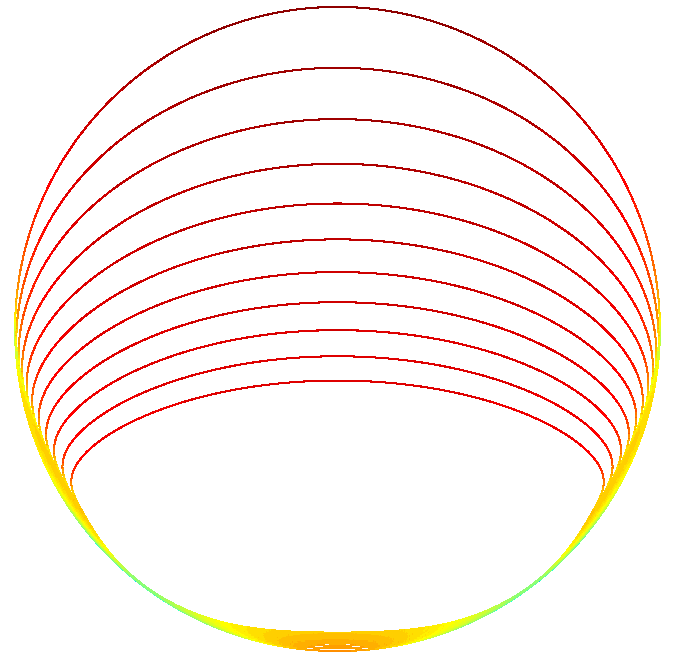
\includegraphics[width = \textwidth]{./figs/1b_0d4r1h_shear}
\caption{}
\end{subfigure}
\begin{subfigure}[b]{0.3\textwidth}
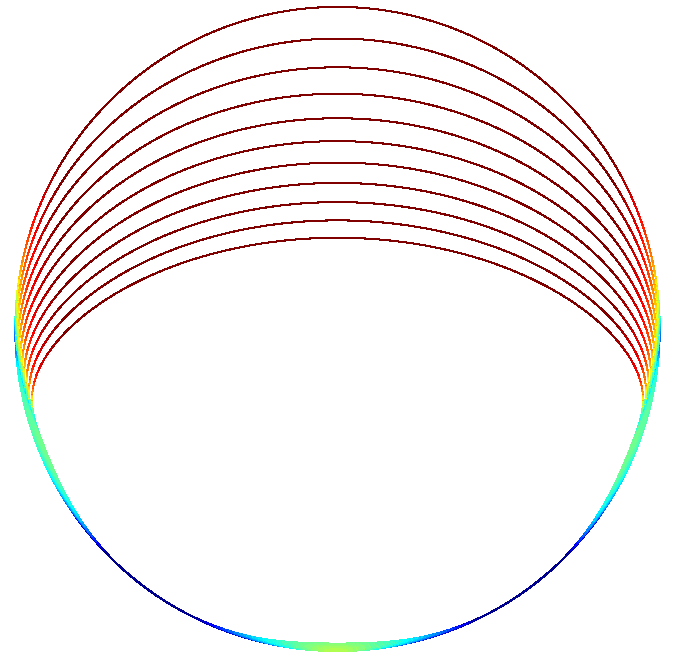
\includegraphics[width = \textwidth]{./figs/1b_0d4r0d5h_shear}
\caption{}
\end{subfigure}
\begin{subfigure}[b]{0.38\textwidth}
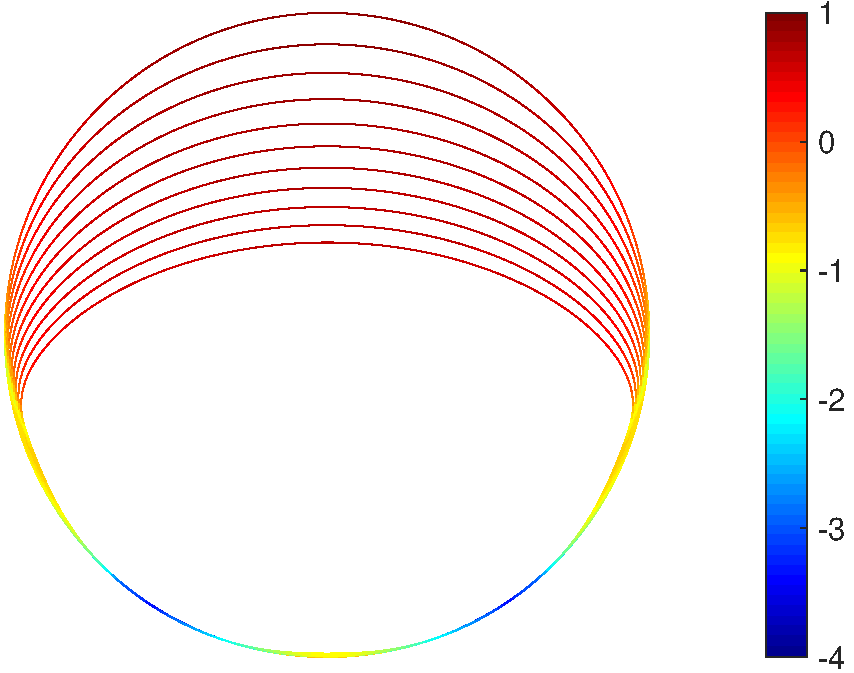
\includegraphics[width =\textwidth]{./figs/1b_0d4r0d1h_shear}
\caption{}
\end{subfigure}
\caption{\label{fig:NearWall} A single body eroding in a Stokes flow.
The color is the logarithm of the shear stress. Therefore, erosion is
fastest in the red regions (upper half) and slowest in the blue regions
(lower half).  The body is initialized at three different distances from
the lower wall: (a) $d=h$, (b) $h/2$, and (c) $h/10$.}
\end{center}
\end{figure}
\begin{figure}[H]
\begin{center}
\begin{subfigure}[b]{0.3\textwidth}
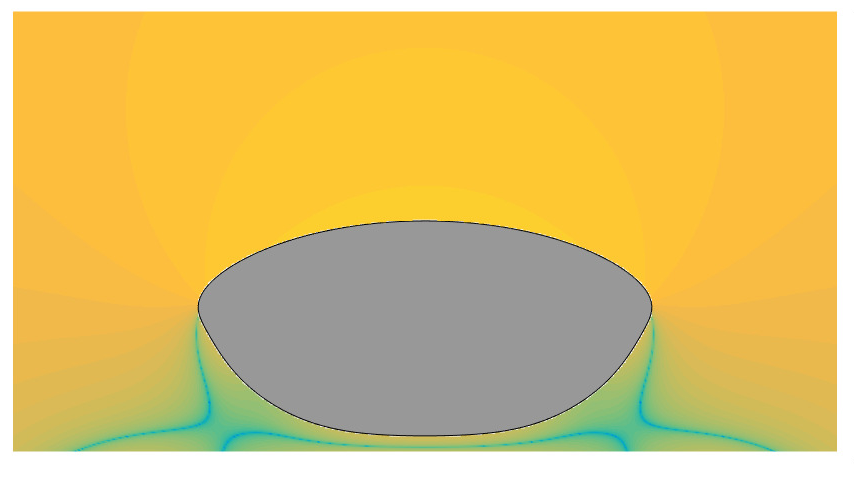
\includegraphics[width = \textwidth]{./figs/1b_0d4r1h_vort}
\caption{}
\end{subfigure}
\begin{subfigure}[b]{0.3\textwidth}
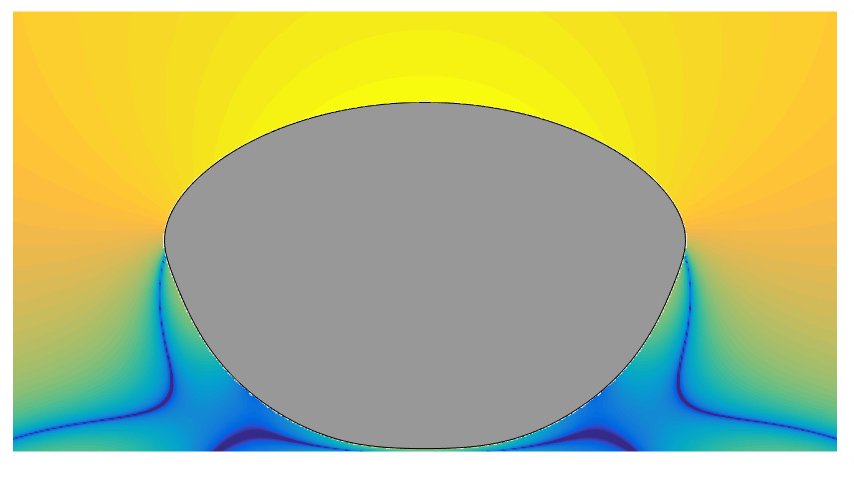
\includegraphics[width = \textwidth]{./figs/1b_0d4r0d5h_vort}
\caption{}
\end{subfigure}
\begin{subfigure}[b]{0.33\textwidth}
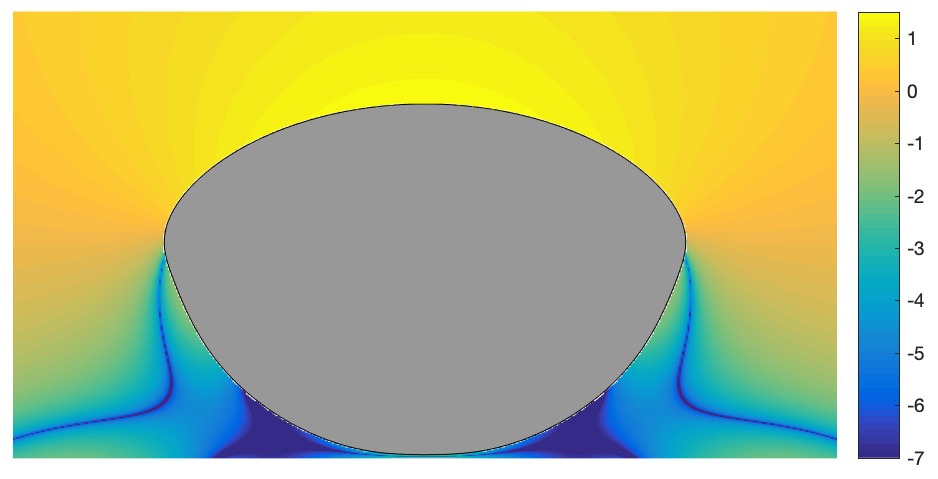
\includegraphics[width = \textwidth]{./figs/1b_0d4r0d1h_vort}
\caption{}
\end{subfigure}
\caption{\label{fig:NearWall_vort} The vorticity of the fluid with a
single body eroding at time t=0.1. The initial distance from the body to
the solid wall are: (a) $h$, (b) $h/2$, and (c) $h/10$.}
\end{center}
\end{figure}


%%%%%%%%%%%%%%%%%%%%%%%%%%%%%%%%%%%%%%%%%%%%%%%%%%%%%%%%%%%%%%%%%%%%%%%
\subsection{20 Bodies at a Medium Porosity}
%%%%%%%%%%%%%%%%%%%%%%%%%%%%%%%%%%%%%%%%%%%%%%%%%%%%%%%%%%%%%%%%%%%%%%%
We consider 20 eroding bodies that are discretized with $N_\iin=256$
points and a time step size of $\Delta t = 10^{-4}$.  The background
flow is the Hagen-Poiseuille flow
\begin{align}
  \UU(\xx)=U \left[
  \begin{array}{c}
    1-y^2 \\ 0
  \end{array}
  \right],
\end{align}
where the flow rate $U$ is chosen so that the pressure drop from $x=-2$
to $x=2$ is held fixed at 2.  Snapshots of the bodies at four equispaced
times are shown in Figure~\ref{fig:Eroding20vort}.  The color is the
vorticity which is equivalent to the shear stress when restricted to the
eroding bodies.  Therefore, the rate of erosion is fastest in regions
where the magnitude of the vorticity is largest.  Initially, several of
the eroding bodies are closer to the outer wall than the $5h$ threshold
required to guarantee that the trapezoid rule achieves machine
precision.  In particular, with $h=L_2/N_\out$, the distance between
bodies 1, 6, 13, and 15 and the outer wall are $1.3h$, $2.9h$, $2.8h$,
and $1.3h$, respectively.  In addition, the distance between several
pairs of eroding bodies is too small to be accurately resolved with the
trapezoid rule at the prescribed resolution.  Particular pairs include
bodies 1 \& 6, 3 \& 9, 6 \& 8, and 14 \& 18.  By using the Barycentric
quadrature rule, the interaction between these nearly-touching bodies
can be accurately resolved at the prescribed resolution, and erosion can
be simulated until all the bodies have vanished.

\begin{figure}[H]
\begin{center}
  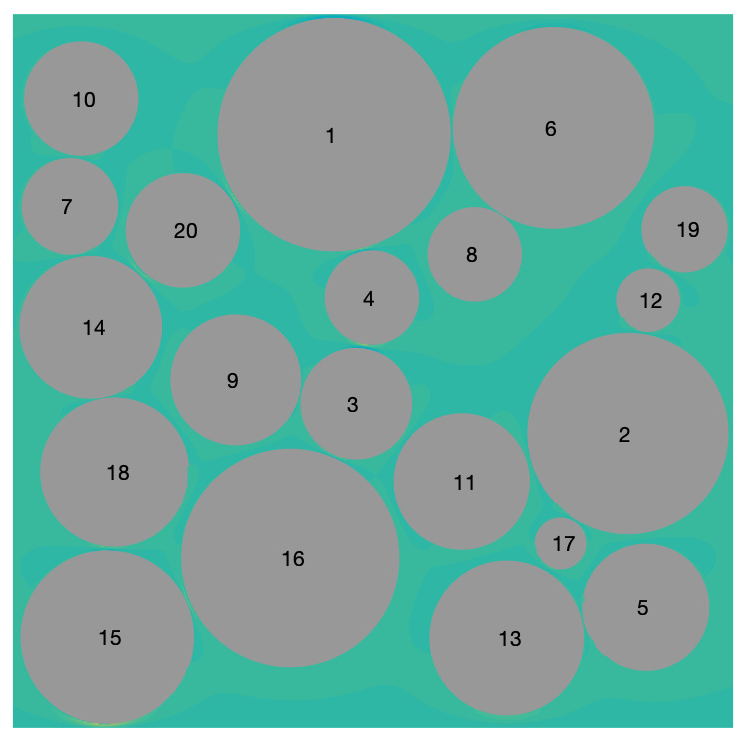
\includegraphics[height=0.225\textwidth]{./figs/20b_dense1}
  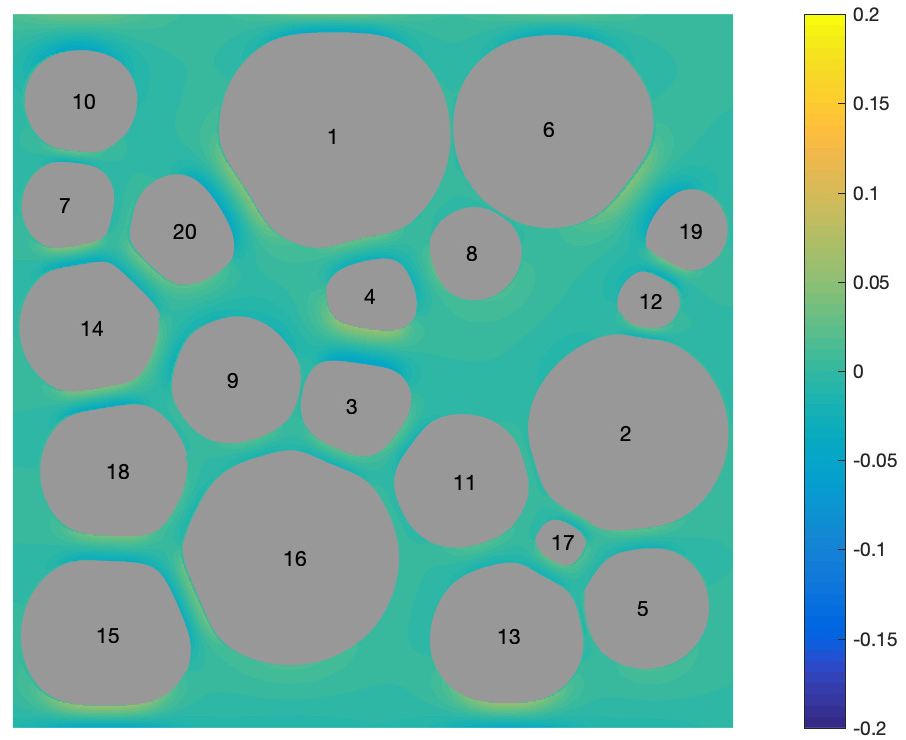
\includegraphics[height=0.225\textwidth]{./figs/20b_dense101}
  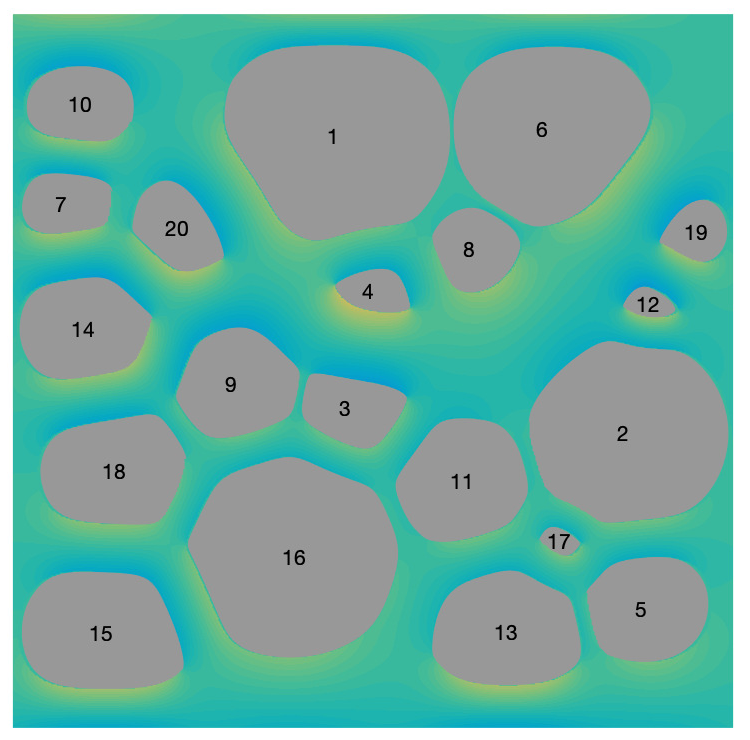
\includegraphics[height=0.225\textwidth]{./figs/20b_dense201}
  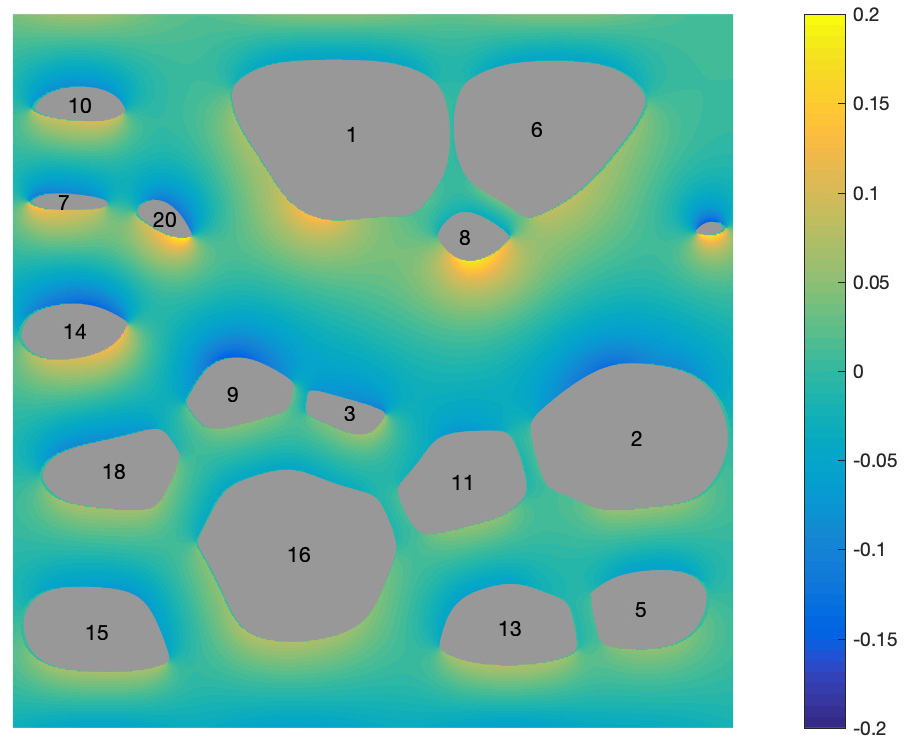
\includegraphics[height=0.225\textwidth]{./figs/20b_dense301}
\caption{\label{fig:Eroding20vort} Erosion of 20 nearly touching bodies
with the fixed pressure drop condition. The color is the vorticity of
the fluid. The four snapshots are evenly spaced in time. We use $N_\iin
= 256$ discretization points on the bodies.  In the fourth frame, bodies
4, 12, and 17 have vanished completely, and body 19 has almost
completely eroded.}
\end{center}
\end{figure}

We observe that erosion creates a network of channels from the inlet to
outlet where the velocity and vorticity, and therefore erosion rate, are
much larger when compared to other regions.  These channels can be
further visualized by considering the streamlines.  In
Figure~\ref{fig:Eroding20tracer}, we freeze the geometry at the second
time step from Figure~\ref{fig:Eroding20vort}, and we plot 200
streamlines that are initialized at $x=-1$ and equispaced in $y$.  The
streamlines are shown at five different times, and the final plot is a
zoom in of the lower right quadrant of the fifth time step.  Since we
use a high-order quadrature rule and a high-order time stepping method,
we resolve streamlines that come very close to the eroded bodies.  There
are three clear regions where the streamlines are concentrated, and this
corresponds to regions of high velocity.  Two of these regions are
located between the bodies and the solid walls at $y=\pm 1$, and the
third cuts through the porous region with the upper part of the channel
formed by bodies 1, 4, 6, and 8.  Since the flow is fastest in these
regions, the shearing is largest, and this causes these openings to grow
fastest which can be observed in Figure~\ref{fig:Eroding20vort}.  

Similar to our previous work, erosion causes the space between nearly
touching bodies to quickly expand, and flat faces develop along the
region of near contact.  This qualitative behavior is present in
Figure~\ref{fig:Eroding20vort} between bodies 3 \& 4, 15 \& 16, and
others.  However, by resolving the interaction betweeen bodies that are
much closer together than in our previous work, we observe that, at
least initially, very little erosion occurs between certain pairs of
bodies.  For instance the opening between bodies 1 \& 6, 3 \& 9, and 5
\& 13 grow much slower than the opening between bodies 15 \& 16.  A
common feature of the openings that grow slowly is that they are nearly
perpendicular to the main flow direction, and this results in a small
velocity, and hence a slow erosion rate.  In fact, when plotting the
streamlines, only a small fraction of the plotted streamlines pass
between theese pairs of bodies indicating a very small velocity.

\begin{figure}[H]
\begin{center}
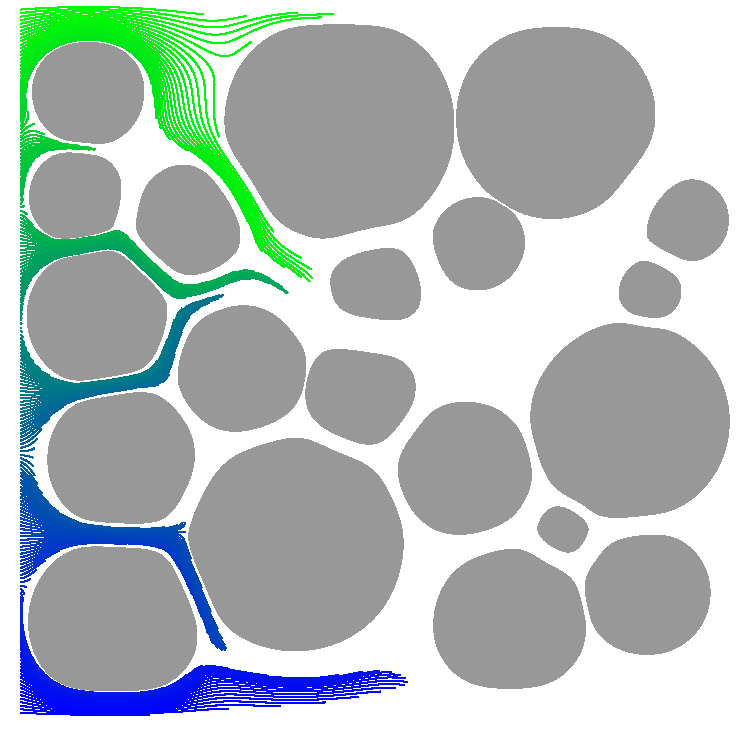
\includegraphics[width = 0.32 \textwidth]{./figs/tracer_20b30}
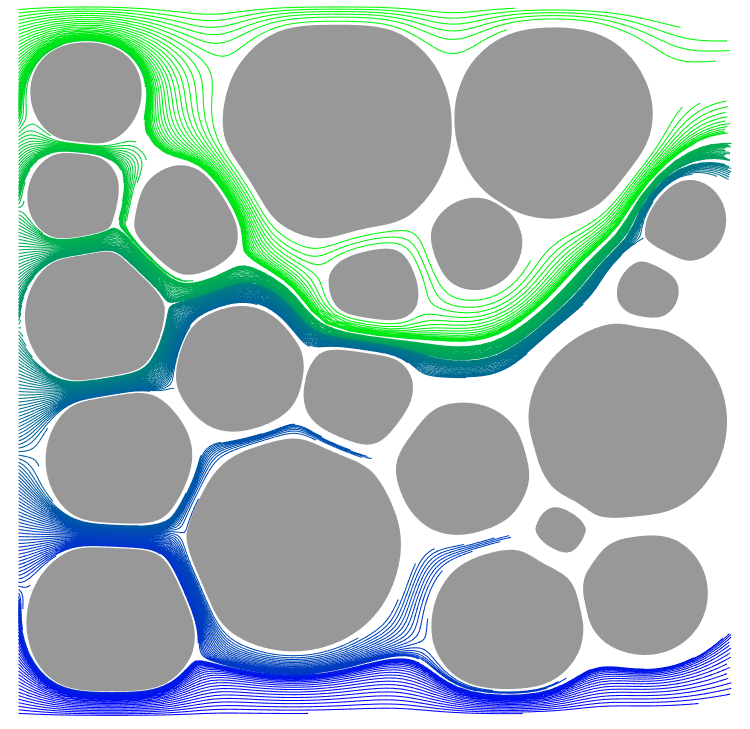
\includegraphics[width = 0.32 \textwidth]{./figs/tracer_20b90}
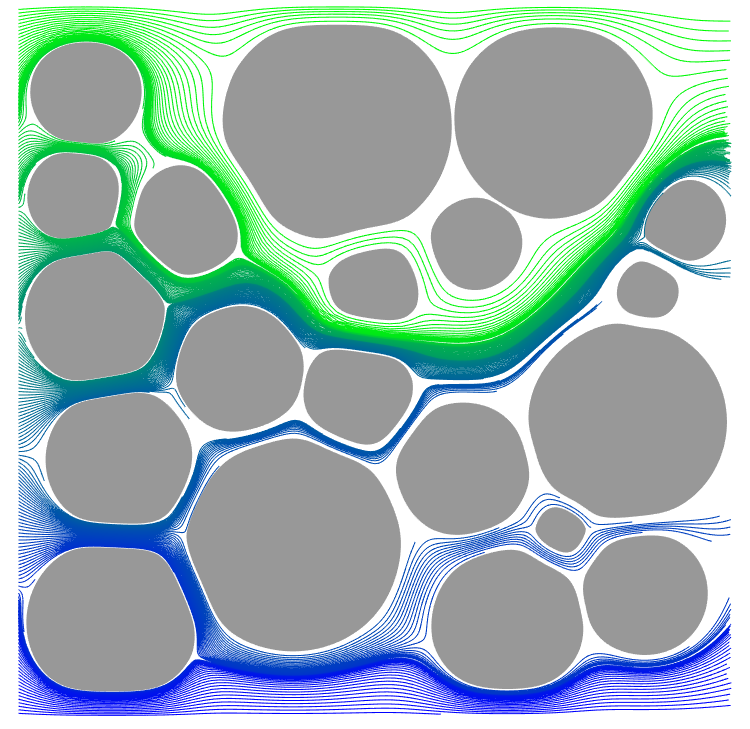
\includegraphics[width = 0.32 \textwidth]{./figs/tracer_20b150}\\
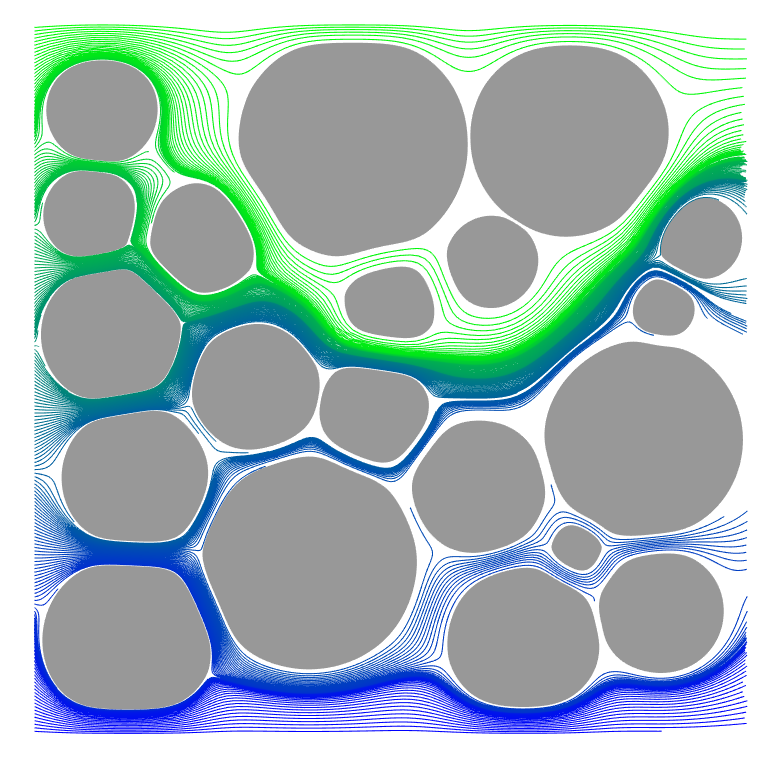
\includegraphics[width = 0.32 \textwidth]{./figs/tracer_20b210}
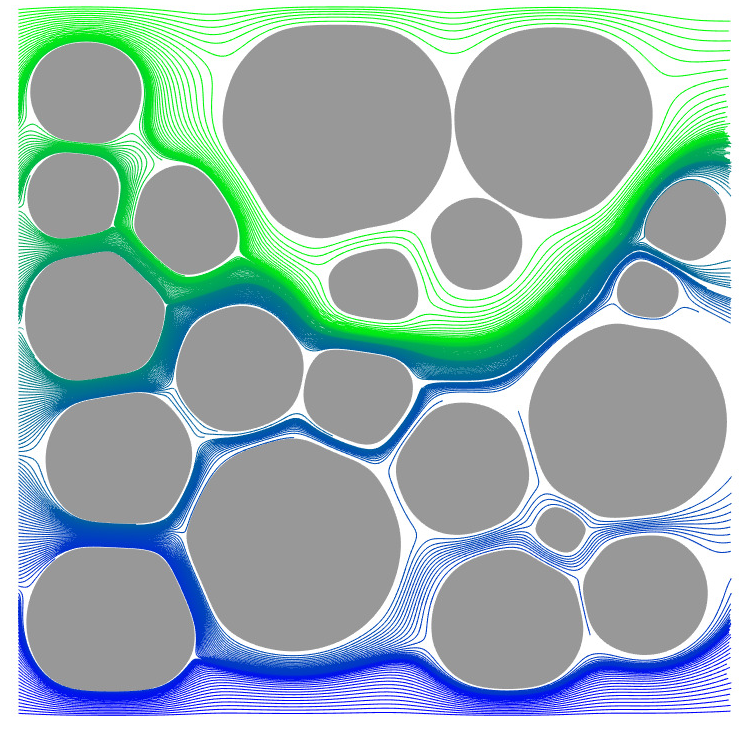
\includegraphics[width = 0.32 \textwidth]{./figs/tracer_20b270}
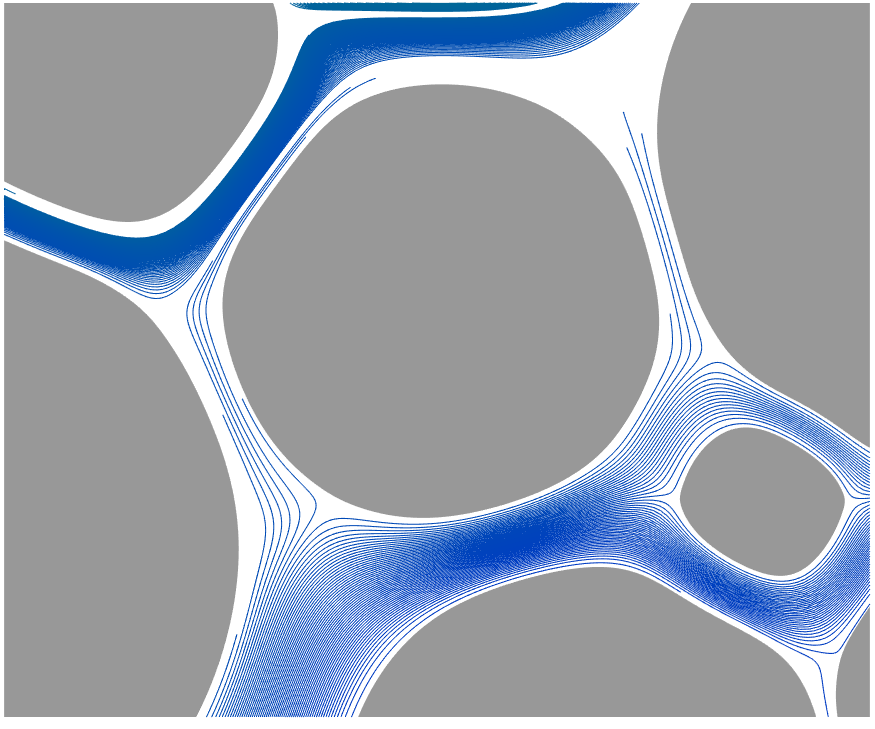
\includegraphics[width = 0.32 \textwidth]{./figs/tracer_20b270_zoom}
\caption{\label{fig:Eroding20tracer} 200 streamlines in the second
geometry from Figure~\ref{fig:Eroding20vort}. The streamlines are
initialized at $x=-1$ and are equally spaced in the $y$-direction. The
first five snapshots are evenly spaced in time.  The bottom right frame
is a zoom in of the fifth snapshot.  Since we use the Barycentric
quadrature rule and the fourth-order Runge-Kutta method, the streamlines
can be very close to but not unphysically penetrate the bodies.}
\end{center}
\end{figure}

Next, we use the streamlines to compute the local tortuosity and the
anomalous dispersion rate of eroding geometries.  Since these
calculations are statistical, we use $N_p = 1000$
streamlines~\cite{bel-sal-rin1992}.  To compute the tortuosity, we
require the velocity at the start of the streamlines.  These normalized
velocities are plotted in Figure~\ref{fig:Eroding20tort}(a) for the
eroded geometry with porosity 62.9\% (see
Figure~\ref{fig:Eroding20tort}(c)).  The velocities are similar to the
work of Matyka et al.~\cite{mat-kha-koz2008} (see Figure 4(a)), except
that our cross-section, by construction, does not cut through any of the
bodies.  Next, in Figure~\ref{fig:Eroding20tort}(b), we plot the local
tortuosity~\eqref{eqn:localTort} by calculating the relative length of
each streamline as it traverses the channel from $x=-1$ to $x=1$.  The
local tortuosity ranges from 1 to 1.27, meaning that one of the
streamlines is 27\% longer than it would have been if the bodies were
absent.  The average streamline length is 9.79\% longer than if the
bodies had been absent, so the tortuosity of the eroded channel is
$1.098$.  Again, comparing the local tortuosity to
Matyka~\cite{mat-kha-koz2008} (Figure 4(b)), the results are
qualitatively similar. However, since our initial cross-section does not
cut through any bodies, the local tortuosity does not have any gaps.
The discontinuities in the local tortuosity happens neighboring
streamlines diverge on opposite sides of a body.  In
Figure~\ref{fig:Eroding20tort}(c), we plot pairs of streamline that
correspond to the ten largest jumps in the local tortuosity.
Corresponding pairs are plotted in the same color.

\begin{figure}[H]
\begin{subfigure}[b]{0.45\textwidth}
\begin{subfigure}[b]{\textwidth}
\includegraphics*[width =\linewidth]{./figs/velocity_loc20_268}
\caption{}
\end{subfigure}
\begin{subfigure}[b]{\textwidth}
\includegraphics*[width =0.97\linewidth]{./figs/tort_local20_268}
\caption{}
\end{subfigure}
\end{subfigure}
\begin{subfigure}[b]{0.5\textwidth}
\includegraphics*[width =\linewidth]{./figs/tort_diff_top10_268}
\caption{}
\end{subfigure}
\caption{\label{fig:Eroding20tort} The tortuosity of an eroded geometry
with porosity 62.9\%. (a) The $x$-component of the velocity, $u(-1,y)$,
normalized by its maximum velocity of $2.98 \times 10^{-3}$. (b) The
local tortuosity $\tau(y)$ along the cross section $x = -1$.  The
spatially averaged tortuosity through the channel is $1.098$.  (c) The
streamlines resulting in the ten largest differences between neighboring
streamlines.  Neighboring streamlines have the same color.}
\end{figure}

In Figure~\ref{fig:Eroding20Transport}(a), we plot the tortuosity as a
function of the porosity from the initial porosity of $0.38$ until all
the bodies have eroded.  The tortuosity is computed with both the length
of the streamlines~\eqref{eqn:tortuosity1} (red marks) and using the
spatial average of the velocity on an Eulerian
grid~\eqref{eqn:tortuosity2} (blue marks).  The red square corresponds
to the porosity of the geometry in Figure~\ref{fig:Eroding20tort}(c).
The two tortuosity formulas give similar results, and any discrepancy
can be accounted for by slow regions of recirculation and quadrature
error induced by the integrals in the tortuosity definitions.  As the
bodies erode, this creates wide channels where streamlines undergo only
minor vertical deflections, and this explains why the tortuosity
eventually decreases with porosity.  We computed lines of best fit using
the porosity-tortuosity models~\eqref{eqn:tortuosityModels}, and the
power law model gave the smallest error.  The  black dashed line in
Figure~\ref{fig:Eroding20Transport}(a) is the line of best fit
\begin{align}
  \widehat{T}(\phi) = \phi^{-0.2064}
\end{align}
with a root-mean-square error of $5.90 \times 10^{-3}$.  The initial
increase in tortuosity occurs because in the absence of erosion (left
plot in Figure~\ref{fig:Eroding20vort}), many of the streamlines, such
as those initialized between bodies 15 \& 18, only perform minor
deflections to pass through the narrow regions, albeit, very slowly.
However, as erosion starts to open the channels, the streamlines deflect
into the fast regions, such as the region above body 11, and this
increases the amount of vertical deflection, and therefore the
tortuosity.

In Figure~\ref{fig:Eroding20Transport}(b), we plot the temporal
evolution of the particle spreading $\sigma_\lambda$.  The spreading is
computed at several geometries that are formed during the erosion
process.  So that the spreading reaches a statistical equilibrium, we
use the reinsertion algorithm described in Section~\ref{sec:dispersion}
to form sufficiently long trajectories.  For all the reported
porosities, the particle dispersion exhibits two power low regimes.
Initially, the dispersion is ballistic ($\sigma_\lambda \sim t$) since
individual fluid particles have not yet explored enough space to
significantly alter their velocity.  However, once the particles have
been subjected to a range of velocities, their dispersion slows down,
and we observe super-diffusive ($\sigma_\lambda \sim t^\alpha$, $\alpha
\in (1/2,1)$) behavior over at least one order of magnitude in time.
Before any erosion takes place, the anomalous dispersion coefficient is
$\alpha = 0.56$.  Then, as the bodies begin to erode, the dispersion
rate grows towards the ballistic regime that corresponds to the absence
of bodies.  The monotonic increase in dispersion with respect to the
porosity is explained by the onset of channels where many tracers
experience less variability in their velocities.

\begin{figure}[H]
\begin{subfigure}[b]{0.5\textwidth}
\includegraphics*[height = 0.8\linewidth]{./figs/tort_eulerian}
\caption{}
\end{subfigure}
\begin{subfigure}[b]{0.5\textwidth}
\includegraphics*[height = 0.8\linewidth]{./figs/20b_second_moment_long_ref}
\caption{}
\end{subfigure}
\caption{\label{fig:Eroding20Transport} (a): The tortuosity of an
eroding geometry initialized with 20 bodies.  The tortuosity is
calculated using the Eulerian method~\eqref{eqn:tortuosity2} (blue dots)
and Lagrangian method~\eqref{eqn:tortuosity1} (red stars).  The red
square correspond to the geometry in Figure~\ref{fig:Eroding20tort}(c).
The dash line is the line of best fit $\widehat{T}(\phi)=\phi^{-p}$ with
$p=0.2064$, and the corresponding root-mean-square error is $5.90 \times
10^{-3}$. (b): The temporal evolution of $\sigma_\lambda$ as a function
of time at seven different porosities.  The dashed line, which has slope
one, corresponds to the ballistic dispersion $\sigma_\lambda \sim t$ if
no bodies were present. At early times, the particles undergo a
ballistic motion, but once they have traversed a few grains, the
dispersion becomes super-dispersive with $\sigma_\lambda \sim t^\alpha$,
$\alpha \in (1/2,1)$.  The dashed-dotted lines are lines of best fit
with slopes $\alpha = 1.06$ ($\phi=95.10\%$), $\alpha = 1.07$
($\phi=85.09\%$), $\alpha = 1.06$ ($\phi=75.15\%$), $\alpha = 0.97$
($\phi=65.09\%$), $\alpha = 0.78$ ($\phi=55.10\%$), $\alpha = 0.75$
($\phi=45.08\%$), and $\alpha = 0.56$ ($\phi=37.68\%$).  Values greater
than 1 are a result of using a least-squares fit for the tails of the
particle spreading.}
\end{figure}

Finally, following our previous work~\cite{qua-moo2018}, we analyze the
effect of erosion on the area fraction and the flow rate.  In
Figure~\ref{fig:Eroding20flowrate}(a), we plot the area fraction as a
function of normalized time.  Initially, 62\% of the geometry contains
eroding bodies corresponding to a porosity of $0.38$, and the area
fraction decreases to 0 as the bodies erode.  The trend of the area
fraction resembles our previous work~\cite{qua-moo2018} (Figure 10(a)),
but with a larger initial area fraction.  In
Figure~\ref{fig:Eroding20flowrate}(b), we plot the flow rate $U$
required to maintain a constant pressure drop across the channel.
Again, the trend of $U$ resembles that of our previous
work~\cite{qua-moo2018} (Figure 10(b)), except that the initial flow
rate is an order of magnitude smaller because of the larger initial area
fraction.  Starting around normalized time $0.2$,
Figure~\ref{fig:Eroding20flowrate}(b) is roughly linear which indicates
that the flow rate can be written as a power law.  Using a line of best
fit, the flow rate is approximately 
\begin{align} 
  U \approx \left(\frac{t}{t_f}\right)^{3.43},
\end{align}
which is the dashed line in Figure~\ref{fig:Eroding20flowrate}(b).

\begin{figure}[H]
\begin{subfigure}[b]{0.5\textwidth}
\includegraphics*[height = 0.7\linewidth]{./figs/porosity20dense}
\caption{}
\end{subfigure}
\begin{subfigure}[b]{0.5\textwidth}
\includegraphics*[height = 0.7\linewidth]{./figs/flow_rate20dense}
\caption{}
\end{subfigure}
\caption{\label{fig:Eroding20flowrate}(a): The area fraction of 20
nearly touching eroding bodies versus normalized time. (b): The flow
rate, $U$, for a fixed pressure drop across the channel versus
normalized time.  The flow rate is initially very small, but it
eventually increases as a power law (dashed line) towards the flow rate
$U=1$ that occurs once all the bodies have eroded.}
\end{figure}

%%%%%%%%%%%%%%%%%%%%%%%%%%%%%%%%%%%%%%%%%%%%%%%%%%%%%%%%%%%%%%%%%%%%%%%
\subsection{20 Bodies at a Low Porosity}
%%%%%%%%%%%%%%%%%%%%%%%%%%%%%%%%%%%%%%%%%%%%%%%%%%%%%%%%%%%%%%%%%%%%%%%
We consider a second example with 20 eroding bodies, but with a smaller
initial porosity.  In Figure~\ref{fig:ErodingLow20vort}, we plot the
eroding geometry and porosity at four evenly spaced instances in time.
Again, the color is the vorticity in the bulk whose magnitude is
equivalent to the erosion rate.   Initially, the smallest distance
between pairs of bodies is $3.29 \times 10^{-4}$, and the smallest
distance between the bodies and solid wall is $4.50 \times 10^{-3}$.  At
these distances, a resolution of approximately $N_\iin = 27,000$ and
$N_\out = 18,000$ discretization points is required to satisfy the $5h$
rule of thumb for the trapezoid rule to achieve machine epsilon
accuracy.  By applying the Barycentric quadrature rule, we stably
simulate erosion at the much coarser resolution of $N_\iin = 256$ and
$N_\out = 1024$ discretization points.

\begin{figure}[H]
\begin{center}
  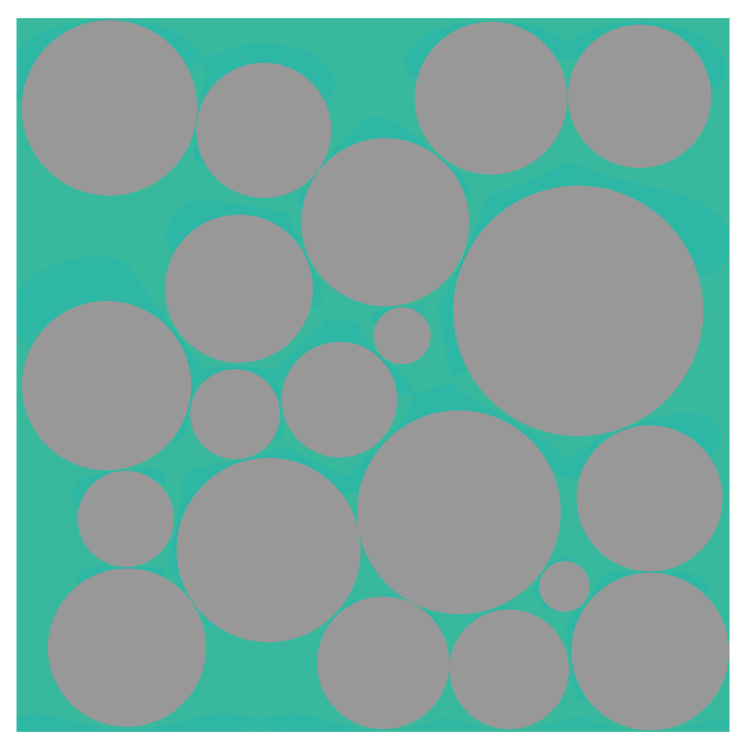
\includegraphics[height=0.225\textwidth]{./figs/20b2_vort1}
  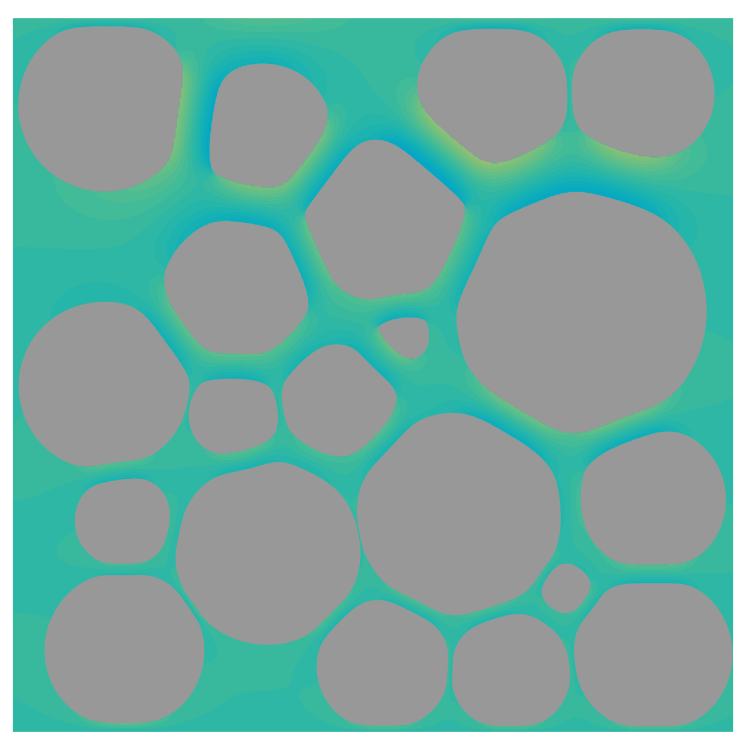
\includegraphics[height=0.225\textwidth]{./figs/20b2_vort150}
  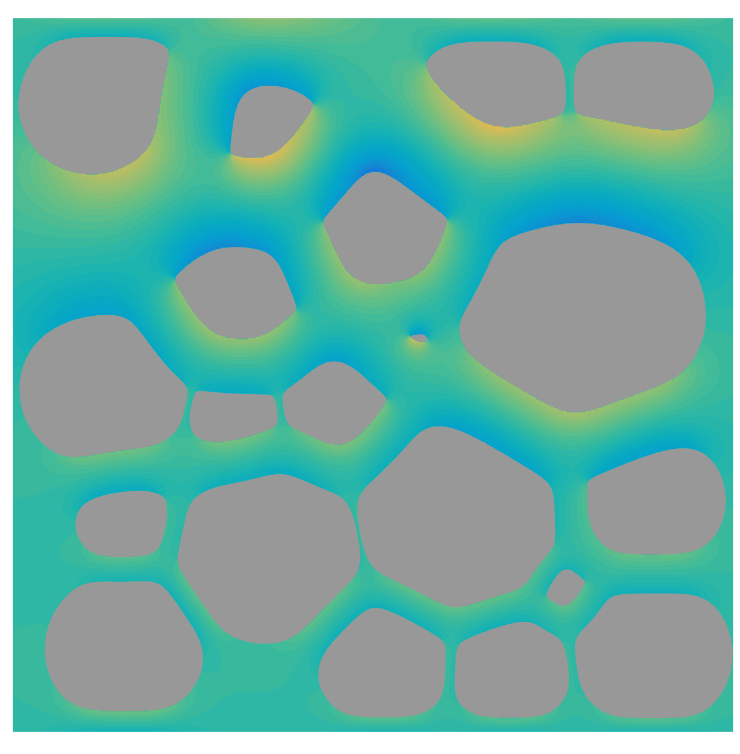
\includegraphics[height=0.225\textwidth]{./figs/20b2_vort300}
  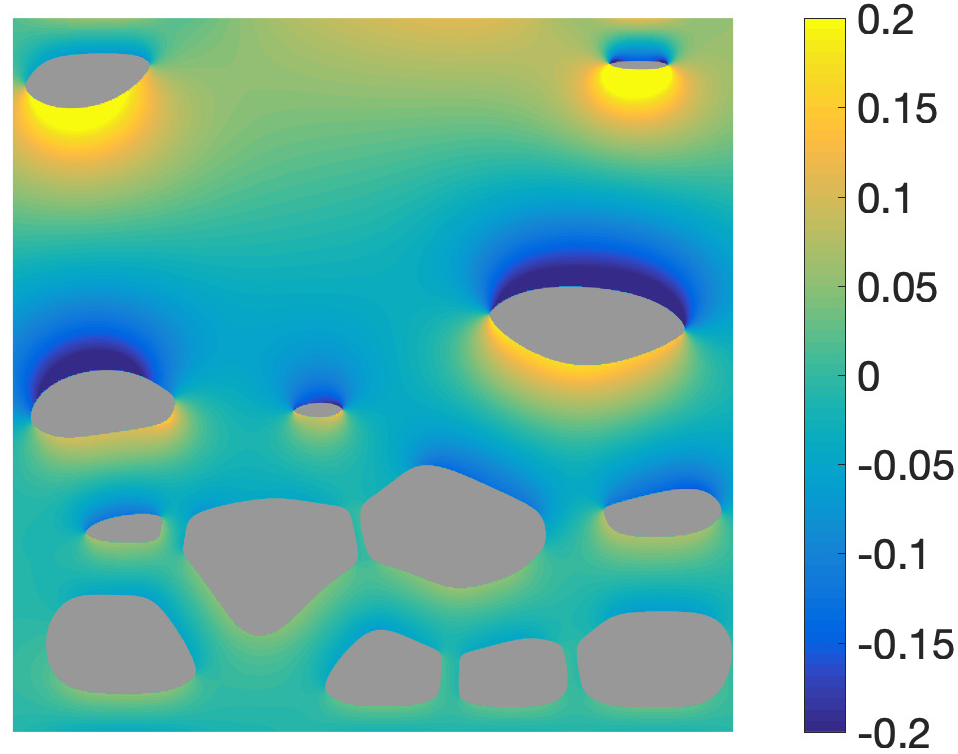
\includegraphics[height=0.225\textwidth]{./figs/20b2_vort450}
\end{center}
\caption{\label{fig:ErodingLow20vort} Erosion of 20 nearly touching
bodies with the fixed pressure drop condition. The color is the
vorticity of the fluid. The 4 snapshots are evenly spaced in time. We
use $N_\iin = 256$ discretization points on the bodies.  In
addition to the channels that develop between the bodies and the solid
walls, Erosion leads to two main channels through the geometry---one in
the top half and one near the middle.}
\end{figure}

We compute the tortuosity using the Eulerian
method~\eqref{eqn:tortuosity2}. In
Figure~\ref{fig:ErodingLow20Transport}(a), we plot the tortuosity with
respect to the porosity (blue) and the line of best fit (black) using
the power law 
\begin{align}
  \widehat{T}(\phi) = \phi^{-0.1669}.
\end{align}
This model outperformed the other three models in
equation~\eqref{eqn:tortuosityModels} that were proposed by Matyka et
al.~\cite{mat-kha-koz2008}.  The root-mean-squared error of the power
law is $1.13 \times 10^{-2}$.  As the bodies erode, the number of
streamlines that take a direct path through the geometry increases,
and this decreases the tortuosity.  However, there is also an increase
in the number of streamlines that increase their length since they
deflect their trajectory to move from a low porosity region (high
pressure) to a high porosity region (low pressure), and this decreases
the tortuosity. For this example, we see that the net effect is a
decrease in the tortuosity for all time.

In Figure~\ref{fig:ErodingLow20Transport}(b), we plot the temporal
evolution of the particle spreading $\sigma_\lambda$.  As in the last
example, we analyze the spreading at several different
porosities and we use the reinsertion algorithm described in Section~\ref{sec:dispersion}
to form sufficiently long trajectories.  For all the reported
porosities, the particle dispersion exhibits two power low regimes, with
the lowest porosity geometry, $\phi=37.68\%$ having the clearest
transition.  Again, the dispersion transforms from a ballistic to
super-diffusive, and the anomalous disperion rate increases with the
porosity.  For this example, the dispersion is nearly Fickean at the
smallest porosity.
\todo[inline]{BQ: This paragraph has some false statements.  Need to
look closer at the data.  Might have accidently been looking at the
other 20 body example ie. Fickean dispersion}

\begin{figure}[H]
\begin{subfigure}[b]{0.5\textwidth}
\includegraphics*[height = 0.8\linewidth]{./figs/tort_eulerian20b}
\caption{}
\end{subfigure}
\begin{subfigure}[b]{0.5\textwidth}
\includegraphics*[height=0.8\linewidth]{./figs/20b_dense_second_moment_ref}
\caption{}
\end{subfigure}
\caption{\label{fig:ErodingLow20Transport} (a): The tortuosity of an
eroding geometry initialized with 20 bodies.  When compared to the last
example, the bodies are initially much closer together, and the porosity
is smaller.  The tortuosity is
calculated using the Eulerian method~\eqref{eqn:tortuosity2} (blue
dots).  The dash line is the fitting line $\widehat{T}(\phi)=\phi^{-p}$
with $p=0.1669$, and the root mean square deviation is $1.13 \times
10^{-2}$.  (b): The temporal evolution of $\sigma_\lambda$ as a function
of time at eight different porosities.  The dashed line, which has slope
one, corresponds to the ballistic dispersion $\sigma_\lambda \sim t$ if
no bodies were present.  At early times, the particles undergo a
ballistic motion, but once they have traveresd a few grains, the
dispersion becomes super-dispersive with $\sigma_\lambda \sim
t^{\alpha}$, $\alpha \in (1/2,1)$.  The dashed-dotted lines are lines of
best fit with slope $0.92$ ($\phi=95.00\%$), $0.87$ ($\phi=85.17\%$),
$0.87$ ($\phi=75.10\%$), $0.91$ ($\phi=65.02\%$), $0.91$
($\phi=55.08\%$), $0.72$ ($\phi=45.03\%$), $0.69$ ($\phi=35.05\%$), and
$0.92$ ($\phi=30.67\%$).}
\end{figure}



%%%%%%%%%%%%%%%%%%%%%%%%%%%%%%%%%%%%%%%%%%%%%%%%%%%%%%%%%%%%%%%%%%%%%%%
\subsection{100 eroding bodies}
%%%%%%%%%%%%%%%%%%%%%%%%%%%%%%%%%%%%%%%%%%%%%%%%%%%%%%%%%%%%%%%%%%%%%%%
As a final example, we consider 100 eroding bodies with an initial
porosity near 55\%.  Snapshots of the configurations and vorticity are
in Figure~\ref{fig:Eroding100vort}.

\begin{figure}[H]
 \begin{subfigure}[b]{0.5\textwidth}
\includegraphics*[width =0.9\linewidth]{./figs/100b_50}
\caption{100 bodies and porosity = 55.54\% at t= 0.005}
\end{subfigure}%
\begin{subfigure}[b]{0.5\textwidth}
\includegraphics*[width =1.1\linewidth]{./figs/100b_100}
\caption{99 bodies and porosity = 62.98\% at t= 0.01}
\end{subfigure}
\begin{subfigure}[b]{0.5\textwidth}
\includegraphics*[width =0.9\linewidth]{./figs/100b_150}
\caption{94 bodies and porosity = 72.22\% at t= 0.015}
\end{subfigure}%
\begin{subfigure}[b]{0.5\textwidth}
\includegraphics*[width =1.1\linewidth]{./figs/100b_200}
\caption{82 bodies and porosity = 83.37\% at t= 0.02}
\end{subfigure}
\caption{\label{fig:Eroding100vort} Erosion of 100 bodies with the
  fixed-pressure-drop condition. The color is the vorticity of fluid. In
  this simulation, we use $N_\iin = 256$ discretization points on the
  body, $N_\out = 1024$ points on the outer wall, a time-step of
  $\Dt=10^{-4}$, and smoothing parameters of $\eps= 15/256$ and
  $\sigma=10/256$.}
\end{figure}

To quantify the tortuosity, we compute the relative velocity
(Figure~\ref{fig:Eroding100tort}(a)) and the local tortuosity
(Figure~\ref{fig:Eroding100tort}(b)) of 1000 tracers placed immediately
to the left of the porous region at $x=-1$.  The porosity at this
instance in time is $62.98\%$ and the maximum velocity at $x=-1$ is
$3.90 \times 10^{-4}$. The initial velocity of the tracers is
qualitatively similar to the 20 body example
(Figure~\ref{fig:Eroding20tort}(a)), except with additional maximum and
minimums because of the additional bodies.  Compared to
Figure~\ref{fig:Eroding20tort}(b), the local tortuosity is much more
discontinuous.  These discontinuities can be explained by examining the
trajectories of tracers in Figure~\ref{fig:Eroding100tort}(c).  Here,
there are many instances of neighboring trajectories that are deflected
apart from one another as they tend to a stagnation point in the flow,
and this results in trajectories with significantly different lengths.
At this instance in time one the tracers travels 25.5\% farther than it
would have if the bodies had been absent, and the average tracer
travelled 12\% farther than it would have if the bodies were absent.
Therefore, at this instance in time, the tortuosity is $1.12$.

\begin{figure}[H]
\begin{subfigure}[b]{0.45\textwidth}
\begin{subfigure}[b]{\textwidth}
\includegraphics*[width =\linewidth]{./figs/velocity_loc100}
\caption{}
\end{subfigure}
\begin{subfigure}[b]{\textwidth}
\includegraphics*[width =\linewidth]{./figs/tort_local100}
\caption{}
\end{subfigure}
\end{subfigure}
\begin{subfigure}[b]{0.5\textwidth}
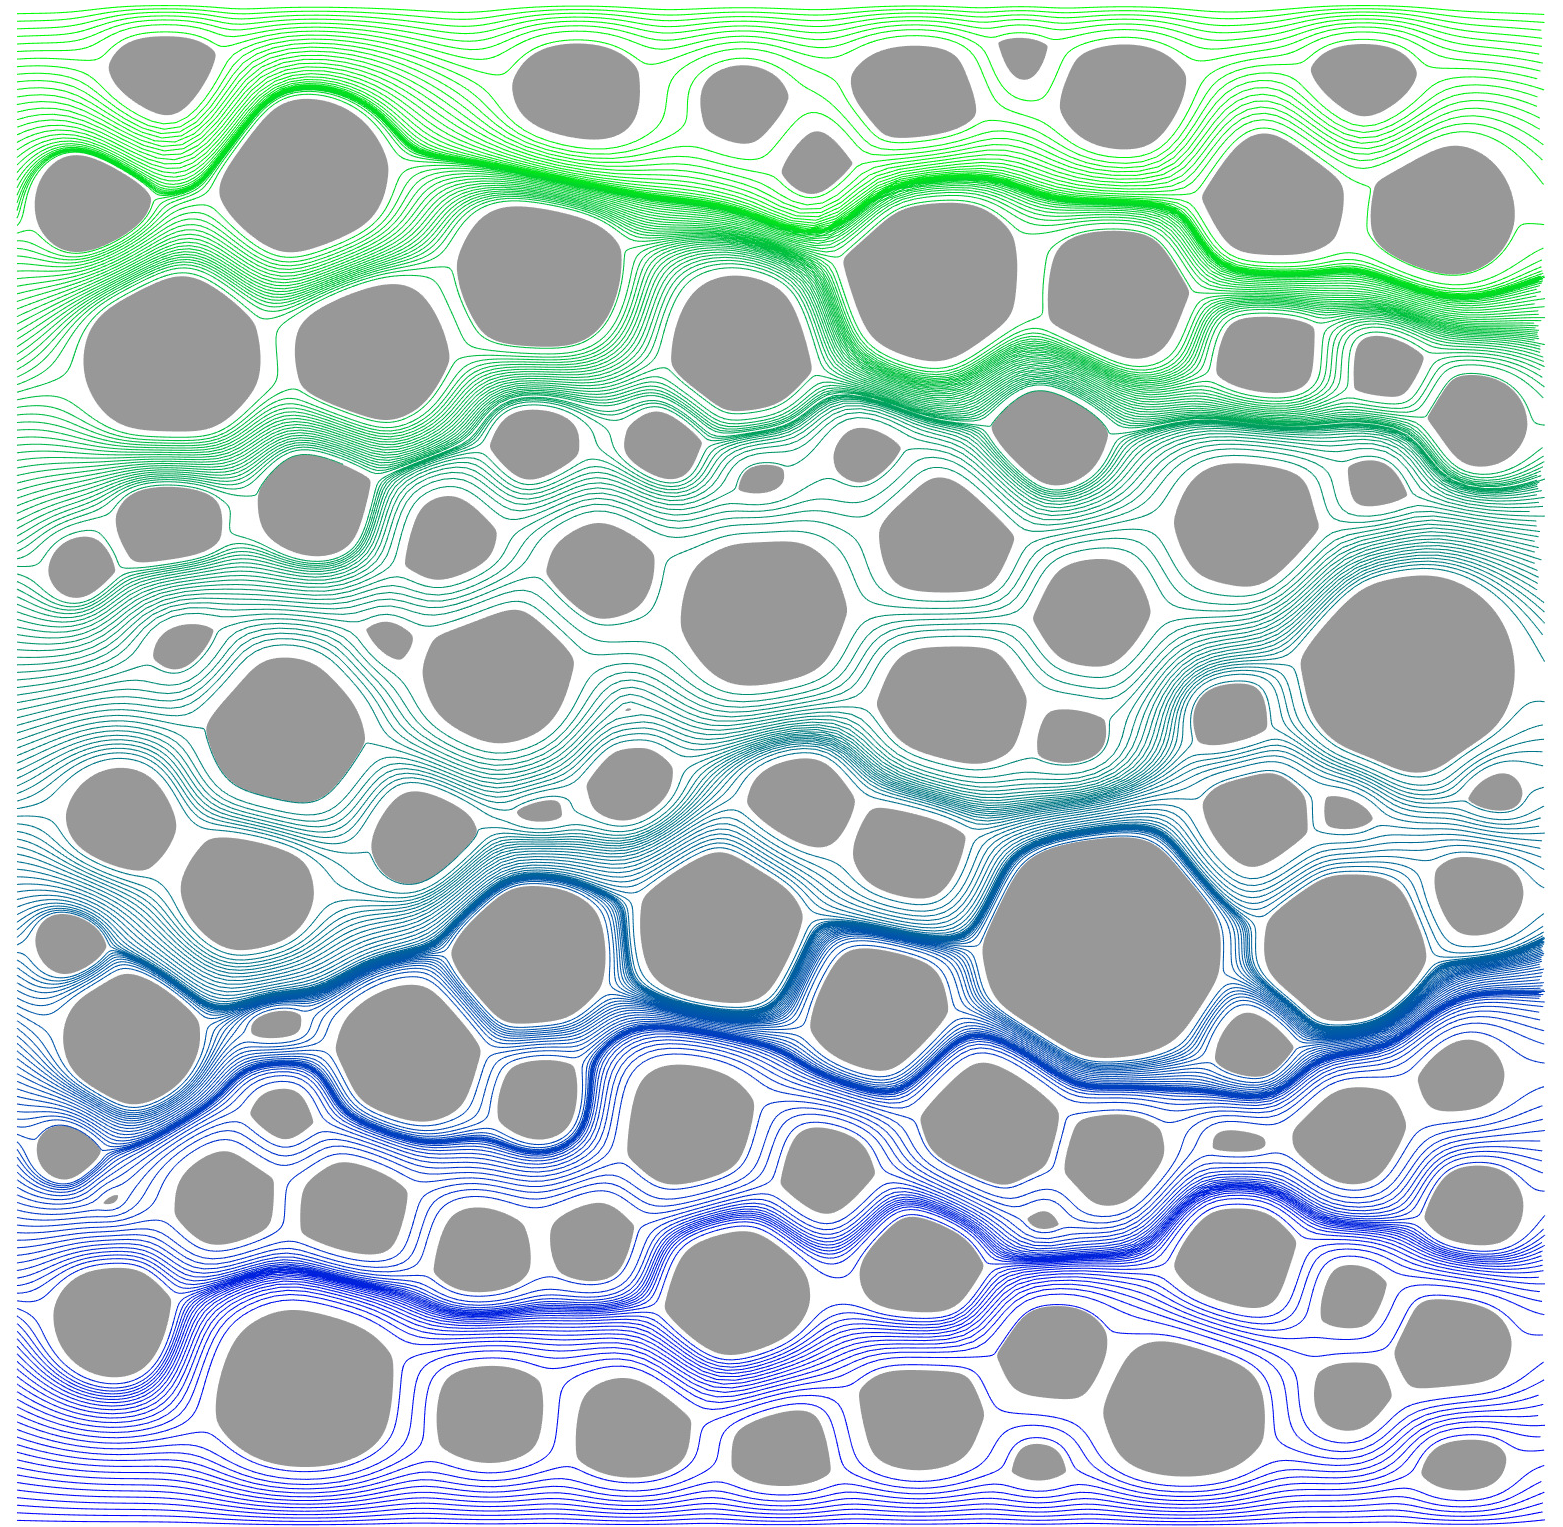
\includegraphics[width = \textwidth]{./figs/100b_t100tracer}
\caption{}
\end{subfigure}
\caption{\label{fig:Eroding100tort} The tortuosity study in the fluid
with 100 bodies when the porosity is 62.98\%.  (a) The x-component
velocity u(-1, y) with respect to its maximum velocity $u_{max}=3.9021
\times 10^{-4}$ at equal spreading tracers on the cross section x = -1.
(b) The local tortuosity $\tau(y)$ on the cross section x = -1. (c) The
trajectories of 200 tracers released at $x = -1$ in the fluid with
multiple bodies.}
\end{figure}

The tortuosity at all porosities from the initial condition until all
the bodies have eroded is in Figure~\ref{fig:Eroding100tort_all}.  The
initial tortuosity is around $T=1.2$ and decays towards $T=1$.  The
tortuosities indicated by the blue dots are calculated using the
Eulerian approach~\eqref{eqn:tortuosity2}, while the red marks use the
Lagrangian approach~\eqref{eqn:tortuosity1}.  Again, the two methods
give comparable results indicating that any recirculation is small and
negligible.  As in the previous examples, the tortuosity depends on the
porosity through a power law model with a small root-mean-squared error
of $5.2 \times 10^{-3}$.  For this example, the logarithm tortuosity
model $\hat{T}(\phi) = 1 - p \ln(\phi)$ achieves a similar
root-mean-squared error.  The tortuosity has one interesting feature
near the end of the simulation where it suddenly increases.  This
behavior can be explained by ... \todo[inline]{S-H: Show me what is
going on here as we discussed.} 

\begin{figure}[H]
\center
\includegraphics*[width =0.55\linewidth]{./figs/tort_eulerian100}
\caption{\label{fig:Eroding100tort_all} The Eulerian and Lagrangian
approach of tortuosity.  The blue dots are Eulerian approach of
tortuosity and the red stars and square are Lagrangian approach of
tortuosity.  The dash line is the fitting line
$\widehat{T}(\phi)=\phi^{-p}$ as $p=0.2459$ and the root-mean-square
error is $5.5 \times 10^{-3}$.  We note that the model
$\widehat{T}(\phi) = 1-p\ln(\phi)$, with $p=0.2631$ has a comparable
root-mean-square error of $5.2 \times 10^{-3}$.}
\end{figure}


Next, we use the 1000 tracer trajectories to compute the second
(Figure~\ref{fig:Eroding100anomalous}) moments of the streamlines at
various porosities.  At high porosities, the first moment is similar to
the first-moment of trajectories in a empty channel (black dashed line).
At smaller porosities, the first moment is always linear, but larger
slopes indicate that the length of the trajectories are longer at lower
porosities \todo[inline]{Don't understand how this is the case}.  The
onset of anomalous dispersion is observed in
Figure~\ref{fig:Eroding100anomalous}. At early times, the particle
spreading is comparable to that of an open channel (dashed curve)
corresponding to the ballistic regime.  However, as the trajectories
traverse the geometry, a transition to a super-dispersive case,
especially at low porosities, is evident.  The dashed-dotted line
corresponds has a slope less than 1 indicating the long time behavior of
the trajectories
\begin{align*}
  \sigma_\lambda \sim t^{0.8715}.
\end{align*}

\begin{figure}
\center
\includegraphics*[width =0.55\linewidth]{./figs/100b_second_moment_long_ref}
\caption{\label{fig:Eroding100anomalous} The analysis of anomalous
dispersion in 100 bodies with respect to initial porosity
(as p=50.09\%) and another five porosities during the eroding. The dashed line
correspondes to a porosity of 100\% and the dashed-dotted lines are lines
of best fit with slope 1.1135 (as p=95.12\%), 0.6825 (as p=85.07\%), 
0.7347 (as p=75.14\%), 0.5915 (as p=65.03\%), 
0.6107 (as p=55.02\%), and 0.7 (as p=50.09\%).}
\end{figure}

Finally, using network models for flow in porous media~\cite{}, the
anomalous dispersion rate can be linked to channel widths between solid
bodies.  We construct a Delaunay triangulation with the centers of the
eroding bodies corresponding to the vertices of the triangles.  Then, if
the side of a triangle connects two vertices, we call the bodies
neighbors.  Then, for each pair of neighbors, we measure the distance
between the bodies.  Once a Delaunay triangulation is formed, it is used
for all subsequent time steps until a body completely disappears.  At
this point, a new Delaunay triangulation is formed.  

We plot the distribution of the gap sizes at four equally spaced points
in time in Figure~\ref{fig:Eroding100gap}.  At the initial configuration, there
are 100 bodies and 318 pairs of neighbors.  The mean distance between
these neighbors is $???  \times 10^{-???}$ and the variance is $???
\times 10^{???}$.  As the bodies erode, the mean and variance of the
distance between the bodies increases.  Finally, at the final time step,
there are only 82 bodies and 254 pairs of neighbors.
\begin{figure}[H]
\begin{subfigure}[b]{0.5\textwidth}
\includegraphics*[width =\linewidth]{./figs/gap_hist100_50}
\caption{100 bodies with 318 gaps at t= 0.005}
\end{subfigure}%
\begin{subfigure}[b]{0.5\textwidth}
\includegraphics*[width =\linewidth]{./figs/gap_hist100_100}
\caption{99 bodies with 312 gaps at t= 0.01}
\end{subfigure}
\begin{subfigure}[b]{0.5\textwidth}
\includegraphics*[width =\linewidth]{./figs/gap_hist100_150}
\caption{94 bodies with 294 gaps at t= 0.015}
\end{subfigure}%
\begin{subfigure}[b]{0.5\textwidth}
\includegraphics*[width =\linewidth]{./figs/gap_hist100_200}
\caption{82 bodies with 254 gaps at t= 0.02}
\end{subfigure}
\caption{\label{fig:Eroding100gap} The distribution of the gaps in the
case of erosion of 100 bodies at four time steps.}
\end{figure}







%\begin{figure}[H]
%\begin{center}
%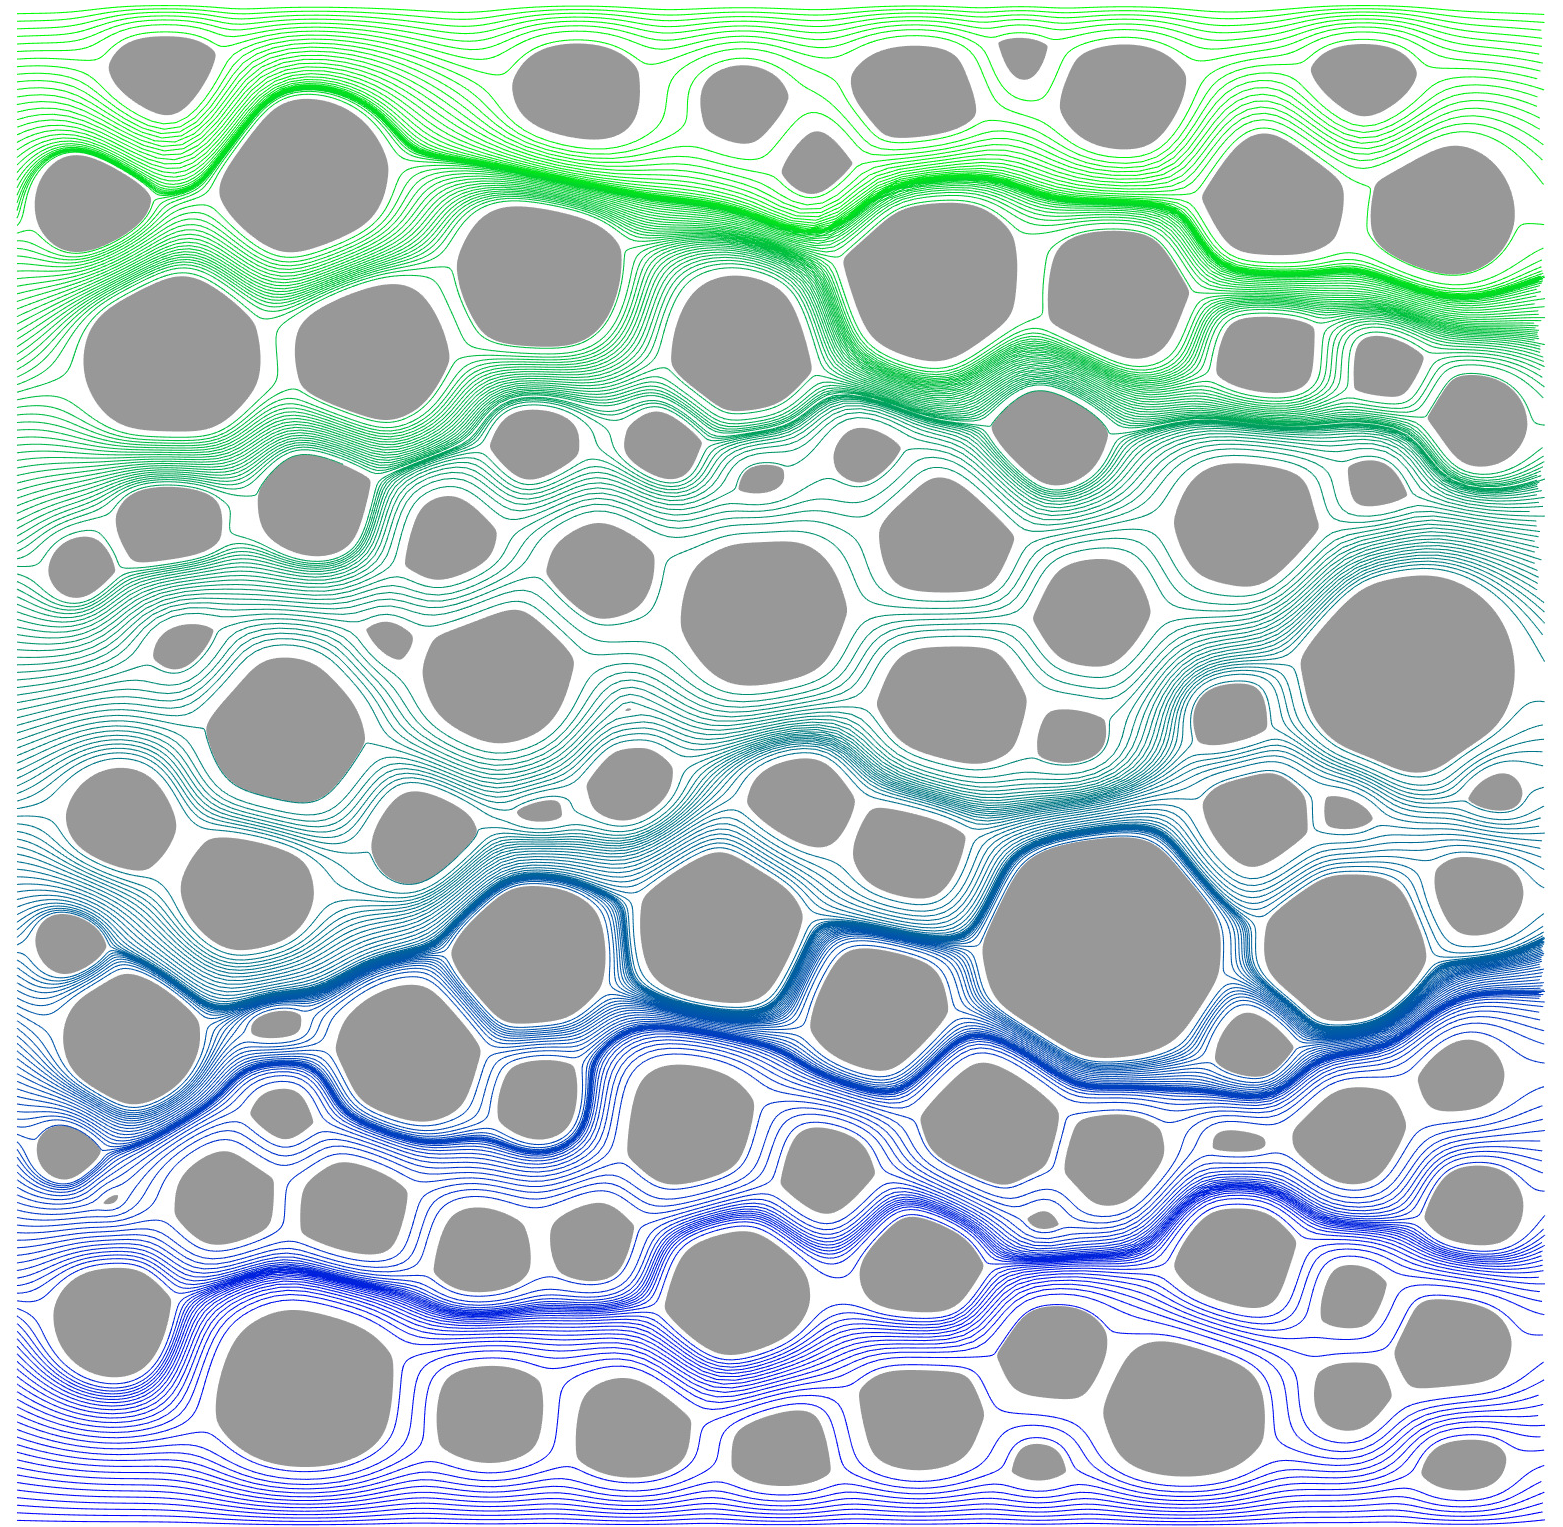
\includegraphics[width = 0.8\textwidth]{./figs/100b_t100tracer}
%\caption{\label{fig:Eroding100tracer} The historical trajectories of 
%200 tracers released at x = -1 in the fluid with multiple bodies.}
%\end{center}
%\end{figure}


%\begin{figure}[H]
%\center
%\includegraphics*[width =0.5\linewidth]{./figs/tort100b_diff_top50}
%\caption{\label{fig:Eroding100tort_traj} The largest 50 difference of 
%local tortuosity $\tau$ at two neighboring tracers in
%100 bodies eroding when the porosity is 62.98 \%
%and the tortuosity is 1.1182. The same color of a pair of trajectories 
%means they are from two neighboring tracers.}
%\end{figure}

%%%%%%%%%%%%%%%%%%%%%%%%%%%%%%%%%%%%%%%%%%%%%%%%%%%%%%%%%%%%%%%%%%%%%%%
\section{Conclusions}
\label{sec:conclusions}
%%%%%%%%%%%%%%%%%%%%%%%%%%%%%%%%%%%%%%%%%%%%%%%%%%%%%%%%%%%%%%%%%%%%%%%


%%%%%%%%%%%%%%%%%%%%%%%%%%%%%%%%%%%%%%%%%%%%%%%%%%%%%%%%%%%%%%%%%%%%%%%
\paragraph{\bf Acknowledgments} BQ and NM were supported by Florida
State University startup funds and Simons Foundation Mathematics and
Physical Sciences-Collaboration Grants for Mathematicians.

\bibliographystyle{plainnat} 
\biboptions{sort&compress}
\bibliography{refs}










%old stuff%
%%%%%%%%%%%%%%%%%%%%%%%%%%%%%%%%%%%%%%%%%%%%%%%%%%%%%%%%%%%%%%%%%%%%%%%%
%\subsection{boundary integral equation formulation} 
%\label{sec:bies}
%add an introduction why we do not use the double-layer potentials of stokes equations but the double-layer potentials of laplace equations to solve stokes equation when we use barycentric approach (or complex variable approach).
%
%\subsubsection{laplace's equations from $\rdb^2$ to $\cdb$ }
%
%let $\omega$ be the domain of fluid. the boundary of $\omega$ is $\gamma$ and the outward normal vector on $\gamma$ is ${\bf n_y}=(n_1,n_2)$.
%
%consider a laplace's equations with dirichlet boundary condition
%\begin{equation}\label{laplace}
%  \begin{cases}
%    \delta {\bf u}=0, & \text{in}\,\,\, \omega \in \rdb^2;\\
%    {\bf u}={\bf f}, & \text{on}\,\,\, \gamma.
%  \end{cases}
%\end{equation}
%
%Let ${\bf x}=(x_1,x_2), {\bf y}=(y_1,y_2)$. Then we have ${\bf r}={\bf x} - {\bf y}$ and $\rho=|\bf r|$.
%The double-layer potential which solves \eqref{Laplace} is 
%\begin{align*}
%\D[\sigma]({\bf x})&=\frac{1}{2\pi}\displaystyle\int_{\Gamma} \frac{{\bf r} \cdot {\bf n_y}}{\rho^2}\sigma({\bf y})ds_y,
%%\frac{1}{2\pi}\displaystyle\int_{\Gamma}\frac{\partial}{\partial {\bf n_y}} \log |{\bf x}-{\bf y}| \sigma({\bf y})ds_y,\\ \\
%%&=\frac{-1}{2\pi}\int_{\Gamma}\frac{{\bf r}\cdot{\bf n_y}}{\rho^2} \sigma({\bf y})ds_y\\ \\
%%&=\frac{-1}{2\pi}\int_{\Gamma}\frac{n_1(x_1-y_1)+n_2(x_2-y_2)}{(x_1-y_1)^2+(x_2-y_2)^2} \sigma({\bf y})ds_y 
%\numberthis\label{DLP:real}
%\end{align*}
%where $\sigma$ is the density function on the boundary $\Gamma$.
%
%
%Consider a Cauchy integral 
%\begin{equation}\label{CI}
%v({x})=\frac{1}{2\pi i}\int_{\Gamma}\frac{\sigma({ y})}{{ y}-{ x}} d{ y},\,\,\,\,\,\,\,\,\, \forall { x} \in \Cdb\setminus \Gamma.
%\end{equation}
%where ${ x}=x_1+ix_2$, $ { y}=y_1+iy_2$, ${ n_y}=n_1+i n_2$ and $d{ y}=i {n_y}ds_y$. It can be shown that 
%the real part of the Cauchy integral in \eqref{CI} is equivalent to the double-layer potential in \eqref{DLP:real}. 
%
%
%\subsubsection{From Stokes DLP to Laplace DLPs}
%
%Let ${\bf x}=(x_1,x_2), {\bf y}=(y_1,y_2)$. Then we have ${\bf r}={\bf x} - {\bf y}$ and $\rho=|\bf r|$.
%
%
%The Stokes double-layer potential  is
%\begin{equation}\label{StokesDLP1}
%\D[\boldsymbol\sigma]({\bf x}):=\frac{1}{\pi}\int_{\Gamma}\left(\frac{{\bf r} \cdot {\bf n_y}}{\rho^2}\frac{{\bf r} \otimes {\bf r}}{\rho^2}\right) {\boldsymbol\sigma({\bf y})} d s_y.
%\end{equation}
%We could rewrite the Stokes DLP in terms of the Laplace DLP as
%\begin{align*}\label{StokesDLP2}
%\D[\boldsymbol\sigma]({\bf x})=\frac{1}{2\pi}\int_{\Gamma}&\frac{{\bf n_y}}{\rho^2}({\bf r} \cdot {\boldsymbol \sigma})ds_y+\frac{1}{2\pi}\nabla\int_{\Gamma}\frac{{\bf r} \cdot {\bf n_y}}{\rho^2}({\bf y} \cdot{\boldsymbol \sigma})ds_y\\
%&-\frac{1}{2\pi}x_1 \nabla\int_{\Gamma}\frac{{\bf r} \cdot {\bf n_y}}{\rho^2}\sigma_1ds_y-\frac{1}{2\pi}x_2\nabla\int_{\Gamma}\frac{{\bf r} \cdot {\bf n_y}}{\rho^2}\sigma_2ds_y. \numberthis
%\end{align*}
%

 
%%%%%%%%%%%%%%%%%%%%%%%%%%%%%%%%%%%%%%%%%%%%%%%%%%%%%%%%%%%%%%%%%%%%%%%%
%\subsection{Computing the shear stress}
%\label{sec:shearStressLP}
%
%To calculate the shear stress, we need to know the gradient of double-layer potential in \eqref{StokesDLP2} 
%\begin{align*}\label{SSLP}
%\nabla\D[\boldsymbol\sigma]({\bf x})=\frac{1}{2\pi}\nabla\int_{\Gamma}&\frac{{\bf n_y}}{\rho^2}({\bf r} \cdot {\boldsymbol \sigma})ds_y+\frac{1}{2\pi}\nabla^2\int_{\Gamma}\frac{{\bf r} \cdot {\bf n_y}}{\rho^2}({\bf y} \cdot{\boldsymbol \sigma})ds_y\\
%&-\frac{1}{2\pi}\nabla\left(x_1 \nabla\int_{\Gamma}\frac{{\bf r} \cdot {\bf n_y}}{\rho^2}\sigma_1ds_y\right)-\frac{1}{2\pi}\nabla\left(x_2\nabla\int_{\Gamma}\frac{{\bf r} \cdot {\bf n_y}}{\rho^2}\sigma_2ds_y\right). \numberthis
%\end{align*}
%
%
%
%
%%%%%%%%%%%%%%%%%%%%%%%%%%%%%%%%%%%%%%%%%%%%%%%%%%%%%%%%%%%%%%%%%%%%%%%%
%\subsection{Boundary evolution in the {\thL} framework} 
%\label{sec:thetaL}
%
%
%%%%%%%%%%%%%%%%%%%%%%%%%%%%%%%%%%%%%%%%%%%%%%%%%%%%%%%%%%%%%%%%%%%%%%%%
%\subsection{Solving the BIE}
%\label{sec:BIE}
%\subsubsection{Interior Case}
%Consider a Cauchy integral 
%\begin{align}\label{CIFI}
%\frac{1}{2\pi i}\int_{\Gamma}\frac{v^-({ y})}{{ y}-{ x}} d{ y}
%&=\begin{cases}
%\,v(x), &{ x} \in \Omega,\\ 
%\,0,  &{ x} \in \Cdb\setminus \bar{\Omega}.
%\end{cases}
%\end{align}
%By the identity of Cauchy Integral Formula $\displaystyle\frac{1}{2 \pi i}\int_{\Gamma}\frac{1}{{ y}-{ x}} d{ y}=1,$ we can rewrtie \eqref{CIFI} and get 
%\begin{equation}
%\frac{1}{2\pi i}\int_{\Gamma}\frac{v^-({ y})-v(x)}{{ y}-{ x}} d{ y}=0,\,\,\,\,\,\,\,\,\, \forall { x} \in \Omega.
%\end{equation}
%\begin{equation}\label{dNCI}
%v'({x})=\frac{1}{2\pi i}\int_{\Gamma}\frac{v^-({ y})}{(y- x)^2} d{ y},\,\,\,\,\,\,\,\,\, \forall { x} \in \Omega.
%\end{equation}
%By the identity of Cauchy Integral Formula $\displaystyle\frac{1}{2 \pi i}\int_{\Gamma}\frac{1}{( y- x)^n} d{ y}=0$ for integer n $\neq 1$, we can rewrtie \eqref{dNCI} and get 
%\begin{equation}
%\frac{1}{2\pi i}\int_{\Gamma}\frac{v^-({ y})-v(x)-(y-x)v'(x)}{(y-x)^2} d{ y}=0,\,\,\,\,\,\,\,\,\, \forall { x} \in \Omega.
%\end{equation}
%
%\subsubsection{Exterior case}
%Consider a Cauchy integral formula for the exterior domain
%\begin{align}\label{CIFE}
%\frac{1}{2\pi i}\int_{\Gamma}\frac{v^+({ y})}{{ y}-{ x}} d{ y}
%&=\begin{cases}
%\,v_{\infty}, &{ x} \in \Omega,\\ 
%\,-v(x)+v_{\infty},  &{ x} \in \Omega^c,
%\end{cases}
%\end{align}
%where $v_{\infty}=\displaystyle\lim_{x \to \infty}v(x)$.
%\begin{equation}
%\frac{1}{x-a}=\frac{-1}{2 \pi i} \int_{\Gamma}\frac{(y-a)^{-1}}{y-x} d{ y},\,\,\,\,\,\,\,\,\, \forall { x} \in \Omega^c.
%\end{equation}
%\begin{equation}
%\frac{1}{2\pi i}\int_{\Gamma}\frac{v^+({ y})-(y-a)^{-1}(x-a)v(x)}{y-x} d{ y}=0,\,\,\,\,\,\,\,\,\, \forall { x} \in \Omega^c.
%\end{equation}
%\begin{equation}
%\frac{1}{2\pi i}\int_{\Gamma}\frac{v^+({ y})-v(x)-(y-a)^{-1}(x-a)(y-x)v'(x)}{(y-x)^2} d{ y}=0,\,\,\,\,\,\,\,\,\, \forall { x} \in \Omega^c.
%\end{equation}
%
%%%%%%%%%%%%%%%%%%%%%%%%%%%%%%%%%%%%%%%%%%%%%%%%%%%%%%%%%%%%%%%%%%%%%%%%
%\subsection{Shear stress}
%\label{sec:shearStress}
%\subsubsection{Interior Case}
%\begin{equation}\label{ddNCI}
%v''({x})=\frac{1}{2\pi i}\int_{\Gamma}\frac{2v^-({ y})}{(y- x)^3} d{ y},\,\,\,\,\,\,\,\,\, \forall { x} \in \Omega.
%\end{equation}
%By the identity of Cauchy Integral Formula $\displaystyle\frac{1}{2 \pi i}\int_{\Gamma}\frac{1}{( y- x)^n} d{ y}=0$ for integer n $\neq 1$, we can rewrtie \eqref{ddNCI} and get 
%\begin{equation}
%\frac{1}{2\pi i}\int_{\Gamma}\frac{2v^-({ y})-2v(x)-2(y-x)v'(x)-(y-x)^2v''(x)}{(y-x)^3} d{ y}=0,\,\,\,\,\,\,\,\,\, \forall { x} \in \Omega.
%\end{equation}
%\subsubsection{Exterior case}
%\begin{equation}
%\frac{1}{2\pi i}\int_{\Gamma}\frac{2v^+({ y})-2v(x)-2(y-x)v'(x)-(y-a)^{-1}(x-a)(y-x)^2v''(x)}{(y-x)^3} d{ y}=0,\,\,\,\,\,\,\,\,\, \forall { x} \in \Omega^c.
%\end{equation}
%%%%%%%%%%%%%%%%%%%%%%%%%%%%%%%%%%%%%%%%%%%%%%%%%%%%%%%%%%%%%%%%%%%%%%%%
%%% TIME-STEPPING %%
%\subsection{Time-stepping with the {\thL} method} 
%\label{sec:timeStepping}
%
%
%%%%%%%%%%%%%%%%%%%%%%%%%%%%%%%%%%%%%%%%%%%%%%%%%%%%%%%%%%%%%%%%%%%%%%%%
%\section{Post processing quantities of interest}
%\label{s:qoi}
%
%%%%%%%%%%%%%%%%%%%%%%%%%%%%%%%%%%%%%%%%%%%%%%%%%%%%%%%%%%%%%%%%%%%%%%%%
%\subsection{Vorticity}
%%%%%%%%%%%%%%%%%%%%%%%%%%%%%%%%%%%%%%%%%%%%%%%%%%%%%%%%%%%%%%%%%%%%%%%%
%\subsection{Pressure}
%\label{sec:pressure}
%
%%%%%%%%%%%%%%%%%%%%%%%%%%%%%%%%%%%%%%%%%%%%%%%%%%%%%%%%%%%%%%%%%%%%%%%%
%\subsection{Drag}
%\label{sec:drag}
%
%%%%%%%%%%%%%%%%%%%%%%%%%%%%%%%%%%%%%%%%%%%%%%%%%%%%%%%%%%%%%%%%%%%%%%%%
%\subsection{Near-singular integration}
%\label{sec:NSI}
%
%
%{\color{red}
%Here we derive the equations~\eqref{eqn:pderiv1}-\eqref{eqn:pderiv2} 
%and the other two are similar.
%To derive equations~\eqref{eqn:pderiv1} and \eqref{eqn:pderiv2}, 
%we need to apply the fact that if a real function $u$ is equivalent to 
%the real part of a complex varaible function $f$, 
%then we have $\nabla u=(\Re(f'),-\Im(f'))$.
%Let $f_1(x)= v[\tau_1](x)$, $f_2(x)=v'[\yy\cdot\eeta](x)$, $f_3(x)=v'[\eta_1](x)$,
%and $f_4(x)= v'[\eta_2](x)$. Then we can rewrite equation~\eqref{eqn:cauchy1}
%\begin{align*}
%u_1(\xx)&= u_{11}(\xx) +  u_{12}(\xx) +u_{13}(\xx)+u_{14}(\xx) \\
%&=\Re (f_1(x)) + \Re (f_2(x))-x_1\Re (f_3(x)) - x_2\Re (f_4(x)).
%\end{align*}
%To get the gradient of $u_1(x)$, we have
%\begin{align*}
%\nabla u_1(x)&= \nabla u_{11}(x)+\nabla  u_{12}(x) 
%+\nabla u_{13}(x)+\nabla u_{14}(x) \\ \\
%&=\begin{bmatrix}
%\Re(f_1'(x))\\ \\
%-\Im(f_1'(x))
%\end{bmatrix}+
%\begin{bmatrix}
%\Re(f_2'(x))\\ \\
%-\Im(f_2'(x))
%\end{bmatrix}
%+
%\begin{bmatrix}
%-\Re(f_3(x))-x_1\Re(f_3'(x))\\ \\
%x_1\Im(f_3'(x))
%\end{bmatrix}
%+
%\begin{bmatrix}
%-x_2\Re(f_4'(x))\\ \\
%-\Re(f_4(x))+x_2\Im(f_4'(x))
%\end{bmatrix}\\ \\
%&=
%\begin{bmatrix}
%\Re (v'[\tau_1](x)) + 
%    \Re (v''[\yy\cdot\eeta](x)) - \Re (v'[\eta_1](x)) - 
%    x_1\Re (v''[\eta_1](x)) - x_2\Re (v''[\eta_2](x))\\ \\
%- \Im (v'[\tau_1](x)) - 
%    \Im (v''[\yy\cdot\eeta](x)) + x_1\Im (v''[\eta_1](x)) - 
%    \Re (v'[\eta_2](x)) + x_2\Im (v''[\eta_2](x))
%\end{bmatrix}.
%\end{align*}
%
%{\color{red}
%\begin{alignat}{3}
%1 &= \frac{1}{2\pi i}\int_{\Gamma} 
%    \frac{1}{y-x} dy, &&x \in \Omega, \label{eqn:cauchyId1}\\
%\frac{1}{x-a} &= \frac{-1}{2\pi i}\int_{\Gamma} 
%    \frac{(y-a)^{-1}}{y-x} dy,  \quad &&x \in \Omega^c\label{eqn:cauchyId2}. 
%\end{alignat}
%and the contour integral 
%\begin{align}\label{eqn:cauchyId3}
%0=\oint_{\Gamma} \frac{1}{(y-x)^n}dy, \quad n \neq 1.
%\end{align}
%Then we apply equations~\eqref{eqn:cauchyId1} and~\eqref{eqn:cauchyId3} on
%the second derivative of Cauchy integral in \eqref{eqn:cauchy} and get
%\begin{align*}
%0 &= \frac{1}{2\pi i} \int_{\Gamma}
%    \frac{2v^-(y)}{(y - x)^3} \, dy -v''(x)\\
%&= \frac{1}{2\pi i} \int_{\Gamma}
%    \frac{2v^-(y)}{(y - x)^3} \, dy 
%-v''(x)\frac{1}{2\pi i}\int_{\Gamma} 
%    \frac{1}{y-x} dy\\
%&= \frac{1}{2\pi i} \int_{\Gamma}
%    \frac{2v^-(y)}{(y - x)^3} \, dy 
%-\frac{1}{2\pi i}\int_{\Gamma} 
%    \frac{(y-x)^2v''(x)}{(y-x)^3} dy
%-\frac{1}{2\pi i}\int_{\Gamma} \frac{2v(x)}{(y-x)^3}dy
%-\frac{1}{2\pi i}\int_{\Gamma} \frac{2(y-x)v'(x)}{(y-x)^3}dy\\
%&= \frac{1}{2\pi i}\int_{\Gamma} 
%    \frac{2v^-({ y})-2v(x)-2(y-x)v'(x)-(y-x)^2v''(x)}{(y-x)^3} dy.
%\end{align*}
%}
%\todo[inline]{S-H: How do we get these identities?}
%\begin{alignat}{3}
%  0 &= \frac{1}{2\pi i}\int_{\Gamma} 
%    \frac{2v^-({ y})-2v(x)-2(y-x)v'(x)-(y-x)^2v''(x)}{(y-x)^3} dy, &&x \in \Omega, \\
%  0 &= \frac{1}{2\pi i}\int_{\Gamma}
%    \frac{2v^+(y)-2v(x)-2(y-x)v'(x)-(y-a)^{-1}(x-a)(y-x)^2 v''(x)}
%    {(y-x)^3} dy, \quad &&x \in \Omega^c.  \label{eqn:Identity}
%\end{alignat}
%{\color{red}
%and the quadrature formulations are
%\begin{alignat}{3}
%  v''(x) &\approx
%    \frac{2\sum\limits_{j=1}^N \frac{v_j^- -v(x)-(y_j-x)v'(x)}{(y_j-x)^3}w_j}
%    {\sum\limits_{j=1}^N \frac{1}{y_j-x}w_j}, &&x \in \Omega, \\
%  v''(x) &\approx \frac{1}{x-a}\frac{2\sum\limits_{j=1}^N
%    \frac{v_j^+ -v(x)-(y_j-x)v'(x)}{(y_j-x)^3}}{\sum\limits_{j=1}^N \frac{(y_j-a)^{-1}}{y_j-x}w_j}
%    , \quad &&x \in \Omega^c.  \label{eqn:SecondBary}
%\end{alignat}
%where $a$ is a point inside the $\Omega$ in equations~\eqref{eqn:Identity} and \eqref{eqn:SecondBary}.
%
%}
%
%{\color{red}
%By using Barycentric quadrature rule to approach integrations, we get a reasonable(?) double-layer potential and quantities of interest at target points but it requires $\mathcal{O}(N^2)$ operations per target point which is computational expensive if we impose it on all the target points. In order to accelerate the process and keep the accuracy, it is a compromise that we use Barycentric quadrature rule to approach the nearly singular integratons but apply trapezoid rule when the target point is far from source points. 
%
%
%To numerically compute the completed double-layer potential, we discretize each of the $M$ bodies with  $N_\iin$ points, and the outer wall with $N_\out$ points. The following is the four-step fast summation methods.
%}
%\begin{itemize}
%  \item Apply trapezoid rule as a first pass
%
%{\color{red} We use the Fast Multipole Method (FMM)~\cite{gre-rok1987, gre-gre-may1992} with trapezoid rule to calculate the double-layer potential.
%}
%  \item Efficiently find points that are too close for trapezoid
%
%{\color{red}
% Let $L_w$ be the length of the outer wall and $L_{b}$ be the length of the boundary of body where $b=1, \cdots, M$. Here are the criteria to see if two points are too close for trapezoid. For criterion of outer wall to body,  let $d$ be the minimum distance between outer wall and a point $x$ on the body $b$, we say $x$ is too close to outer wall if
%\begin{equation}\label{eqn:Cw2b}
%d< \alpha_1\frac{L_w}{N_\out}
%\end{equation}
%where $\alpha_1$ is a constant. 
%For criterion between two bodies, let $d$ be the distance between the centroid $a$ of the body $b_1$ and a point $x$ on the body $b_2$, we say they are too close if
%\begin{equation}\label{eqn:Cb2b}
%d<\alpha_2\left(\frac{L_{b_1}}{N_\iin}+\frac{L_{b_2}}{N_\iin}\right)
%\end{equation}
%where $\alpha_2$ is a constant. 
%
%}
%\end{itemize}
%{\color{red}  (Discussion of the choices of $\alpha_1$ and $\alpha_2$ with respect to accuracy and  efficiency)
%
%To find the suitable values of $\alpha_1$ and $\alpha_2$ in~\eqref{eqn:Cw2b} and \eqref{eqn:Cb2b}, we set $\alpha_1=\alpha_2=1, 2, 3$, and $4$ to test the criteria on a 20-body problem with $N_\out = 1024$ and $N_\iin = 128, 256$, and $512$. To check the accuracy of the simulations, we use the solution calculated by \todo[inline]{what method} to \todo[inline]{...}
%To see how efficient our code is, we record the cpu time for each step.
%
%}

%{\color{red} 
%By using Barycentric quadrature rule, we are able to capture the details
%in the fluid when wall and bodies or body and bodies are close to each
%other.  The first nearly touching bodies case is 20 bodies in a
%Hagen-Poiseuille flow.  The initial velocity of flow from the left side
%of $\Omega$ is $$\UU(\xx)=U\begin{bmatrix} 1-y^2\\ 0\end{bmatrix},$$
%where $U$ is chosen such that the pressure drop between  $x=-2$ and
%$x=2$ remains fixed at 8.  With this choice, the velocity in the absent
%of grains has flow rate $U=1$.  The number of discretization points is
%$N_\iin = 256$.
%
%The snapshots of the process of 20 nearly touching bodies eroding are in
%Fig.~\ref{fig:Eroding20vort}.  We initially place some bodies to nearly
%contact not only one another but also the outer wall. For example,
%bodies 1, 6, 13, and 15 are very close to outer wall: the distance
%between body 1 and outer wall is $1.3025h$, the distance between body 6
%and outer wall is $2.9275h$, the distance between body 13 and outer wall
%is $2.8447h$, the distance between body 15 and outer wall is $1.3352h$
%where $h=L_w/N_\out$ is the arclength spacing correponding to the outer
%wall.  In~\cite{qua-moo2018} we reported the quick expanding space at
%the narrow channel between neighboring bodies, the developing flat faces
%at the sites of near contact, and bodies vanishing. In this nearly
%touching bodies structure, we also observe these similar phenomena but
%not totally the same.  For the speed of expanding space at the narrow
%channel, we see some narrow channels do expand faster than other wider
%channels.  For example, the spacing between bodies 14 and 18 is smaller
%than the spacing between bodies 7 and 14 initially and the former one is
%comparable to the latter one by the second frame. But there are some
%small initial spacings that do not expand that much at all by the fourth
%frame, for example between bodies 1 \& 6, 3 \& 9.  We could find the
%explanation from the vorticity of fluid in Fig.~\ref{fig:Eroding20vort}.
%Since the eroding velocity on the body is proportional to the absolute
%value of vorticity in our erosion model,  then when the  absolute value
%of vorticity is small there is not much erosion on the body.  In all
%four frames of Fig.~\ref{fig:Eroding20vort}, the vorticity is relatively
%small between bodies 1 \& 6 and 3 \& 9.
%
%Besides the channels between two bodies, there is a single channel goes
%across the domain horizontally and the flow has been concentrated in
%this channel.  In the second frame of Fig.~\ref{fig:Eroding20vort}, this
%channel is between bodies 1 \& 20, 1 \& 9, 4 \& 3, 8 \& 11, 8 \& 2, 6 \&
%12, and 6 \& 19.  We can get a better understanding of this channel from
%the trajectories of tracers in Fig.~\ref{fig:Eroding20tracer}.  In the
%top three frames of  Fig.~\ref{fig:Eroding20tracer}, the flow (or
%tracer) first comes from three small channels between outer wall \& body
%10, bodies 7 \& 14, and bodies 14 \& 18, then the three branches become
%one and go into the main channel between bodies 1 \& 9.  From the first
%frame to the forth frame of Fig.~\ref{fig:Eroding20vort}, this channel
%is expanding faster than other channel and bodies 4 \& 12 has vanished
%and body 19 is almost gone in the forth frame.  The reason of fast
%expansion of this channel is the high vorticity.  In the forth frame of
%Fig.~\ref{fig:Eroding20vort}, we could see the vorticity is relatively
%high on the side of bodies which form this channel so the bodies are
%eroded fast on the side of this channel or have vanished completely.
%
%Furthermore, how long the body lasts for depends on not only the size of
%the body but also the location of the body.  For example, the first
%three vanishing bodies are body 12 (as t=0.0256), 4 (as t=0.0278), then
%17 (as t=0.0287).  Since body 4 is located in the main flow channel so
%the body 4 is vanished earlier than body 17 although the initial size of
%body 4 is larger than the size of body 17.  This channel will keep
%expanding and the bodies around this channel will vanish earlier than
%others.  After body 17, the next 8 vanished bodies with respect to time
%are body 19 (as t=0.0312),  body 7 (as t=0.0325), body 20 (as t=0.0329),
%body 8 (as t=0.0349), body 10 (as t=0.0353), body 3 (as t=0.0356), body
%14 (as t=0.0363), then body 9 (as t=0.0376).  All of these eight bodies
%were around this channel before they are gone.
%
%For the flat faces at the sites of near contact, since we put the body
%be close to one another so we are able to see all the channels between
%two close bodies have flat faces.  Besides the channels between bodies,
%we also observe the flat faces on the bodies which are close to the
%outer wall. For example, we see the flat faces on the top of bodies 1 \&
%6 and the bottom of bodies 13 \& 15.  
%
%Since we use a Barycentric quadrature rule to approximate the velocity
%of tracers and apply the fourth order Runge Kutta method to find the new
%locations of tracers in each step, the tracers can be very close to but
%not penetrate the bodies.  Those body-closed tracers are moving
%perfectly so we are able to observe the details of the interaction of
%bodies and fluid.  Although the direction of flow is from left to right,
%the tracers will not only travel horizontally but also vertically.  In
%the last three frames of Fig.~\ref{fig:Eroding20tracer}, some tracers
%climb up from right to left around the body.  There are zoom windows of
%the climbing tracers trajectories in Fig.~\ref{fig:Eroding20zoom} and
%they are taken from the last three frames of
%Fig.~\ref{fig:Eroding20tracer} with more tracers.  In
%Fig.~\ref{fig:Eroding20zoom} the tracers around the center body first go
%from the channel below the body, climb up to the left, then go to the
%right and join another tracers in the channel above the body. 
%
%In Fig.~\ref{fig:Eroding20area} and Fig.~\ref{fig:Eroding20flowrate} we
%measure the area occupied by bodies and the flow rate $U$ quantifily
%during the eroding. In the beginning, 62.32\% of area of $[-1,1] \times
%[-1,1]$ is occupied by 20 bodies. Then the eroding speed is increasing
%when more and more bodies are vanished in the fluid. 
%
%The flow rate increases exponentially with growth rate close to
%$\ln10^4$. 
%
%
%In Fig.~\ref{fig:Eroding20tort} we use tortuosity to analysis the effect
%of the geometrical structure on fluid velocity field. In
%Fig.~\ref{fig:Eroding20tort}(a) the graph represents the ratio of the
%x-component velocity u(-1, y) to its maximum velocity $u_{max}=6.2281
%\times 10^{-4}$ at equal spreading tracers on the cross section (x=-1
%and y in [-1,1]). The velocity is continuous along the cross section and
%acting as several Poiseuille flows. This velocity graph is different
%from the one in~\cite{matyka2008tortuosity} since we choose our cross
%section to be the beginning of the flow before the fluid touches any
%body. In Fig.~\ref{fig:Eroding20tort}(b) we record the local tortuousity
%$\tau$ of the tracers at the cross section. This graph is not continuous
%and the jumps in $\tau$ mean that the initial neighbor tracers have been
%seperated by the bodies. 
%
%In Fig.~\ref{fig:Eroding20tort}(c)
%In Fig.~\ref{fig:Eroding20tort}(d) 
%}
%
%{\color{red}
%To study the interaction of fluid and fixed bodies in the porous media,
%some parameters can be used to describle the interation quantitively,
%for example the porosity, the permeability, and the tortuosity. 
%The relation of porosity and tortuosity has been studied in~\cite{matyka2008tortuosity}.
%The definition of porosity is the ratio 
%$$\phi=\frac{A_v}{A_T}$$
%where $A_v$ is the area of void-space and $A_T$ is the area of the calculating area.}
%{\color{red} The tortuosity represents the weighted average travel distance of a tracer in a porous media. 
%The definition of tortuosity is 
%$$T=\frac{1}{d}\frac{\displaystyle\int_{S}u_x(y) \lambda(y)dy}{\displaystyle\int_{S}u_x(y)dy}$$
%where $S$ is an arbitrary cross section which is perpendicular to the x axis,
%$\lambda(y)$ is the length of streamline at y on $S$, 
%$u_x(y)$ is the component of velocity at y which is normal to $S$, and 
%$d$ is the distance from $S$ to the end cross section.
%It depends on not only the geometric structure but also the velocity of the fluid 
%which is different from the porosity since porosity only depends on the geometric structure.}
%{\color{red}Beisdes, the local tortuosity~\cite{matyka2008tortuosity} has been used to analysis 
%the local behavior of steamline around a body. 
%The definition of local tortuosity of the tracers at $y$ on $S$ is
%$$\tau(y)=\frac{\lambda(y)}{d}.$$ 
%}

%%%%%%%%%%%%%%%%%%%%%%%%%%%%%%%%%%%%%%%%%%%%%%%%%%%%%%%%%%%%%%%%%%%%%%%%
%\subsection{Cauchy Integral Representation of the Pressure}
%%%%%%%%%%%%%%%%%%%%%%%%%%%%%%%%%%%%%%%%%%%%%%%%%%%%%%%%%%%%%%%%%%%%%%%%
%The pressure of the double-layer potential is
%\begin{align}
%  p(\xx) = -\frac{1}{\pi} \int_{\bd\Omega} \frac{1}{\rho^2}
%    \left(1 - 2 \frac{\rr \otimes \rr}{\rho^2} \right) \nn
%    \cdot \eeta(\yy) \, ds_\yy.
%\end{align}
%
%
%
%{\color{red}
%We
%measure the area occupied by bodies 
%during the eroding and record the flow rate $U$ quantifily in log scale
%during the eroding in Fig.~\ref{fig:Eroding20flowrate}. 
%Since we simulate the erosion by applying fixed pressure drop 
%the flow rate $U$ is small when there are many bodies in the fluid and 
%when the area fraction is getting smaller $U$ is getting larger.
%In Fig.~\ref{fig:Eroding20flowrate}, 62.32\% of area of $[-1,1] \times
%[-1,1]$ is occupied by 20 bodies initially and the flow rate $U$ starts from $9.86\times 10^{-5}$. 
%Then the eroding speed is increasing
%when more and more bodies are vanished in the fluid and 
%the maximum eroding speed happens when the area fraction equals 7.57\% 
%which is occupied by 8 bodies.
%When all the bodies have vanished completely the flow rate $U$ is equal to 1.
%In Fig.~\ref{fig:Eroding20flowrate}(b), the flow rate $U$ increases exponentially 
%with growth rate close to $\ln10^4$. }
%Besides the channels between two bodies, there is a single channel goes
%across the domain horizontally and the flow has been concentrated in
%this channel.  In the second frame of Fig.~\ref{fig:Eroding20vort}, this
%channel is between bodies 1 \& 20, 1 \& 9, 4 \& 3, 8 \& 11, 8 \& 2, 6 \&
%12, and 6 \& 19.  We can get a better understanding of this channel from
%the trajectories of tracers in Fig.~\ref{fig:Eroding20tracer}.  In Fig.~\ref{fig:Eroding20tracer}, 
%the flow (or tracer) first comes from three small channels between outer wall \& body
%10, bodies 7 \& 14, and bodies 14 \& 18, then the three branches become
%one and go into the main channel between bodies 1 \& 9.  From the first
%frame to the forth frame of Fig.~\ref{fig:Eroding20vort}, this channel
%is expanding faster than other channel and bodies 4 \& 12 has vanished
%and body 19 is almost gone in the forth frame.  The reason of fast
%expansion of this channel is the high vorticity.  In the forth frame of
%Fig.~\ref{fig:Eroding20vort}, we could see the vorticity is relatively
%high on the side of bodies which form this channel so the bodies are
%eroded fast on the side of this channel or have vanished completely.
%{\color{red} 
%Furthermore, how long the body lasts in the fluid depends on not only
%the size of the body but also the location of the body.  For example,
%the first three vanishing bodies are body 12 (as t=0.0256), 4 (as
%t=0.0278), then 17 (as t=0.0287).  Since body 4 is located in the main
%flow channel so the body 4 is vanished earlier than body 17 although the
%initial size of body 4 is larger than the size of body 17.  This channel
%will keep expanding and the bodies around this channel will vanish
%earlier than others.  After body 17, the next 8 vanished bodies with
%respect to time are body 19 (as t=0.0312),  body 7 (as t=0.0325), body
%20 (as t=0.0329), body 8 (as t=0.0349), body 10 (as t=0.0353), body 3
%(as t=0.0356), body 14 (as t=0.0363), then body 9 (as t=0.0376).  All of
%these eight bodies were around this channel before they are gone.
%
%For the flat faces at the sites of near contact, since we put the body
%be close to one another so we are able to see all the channels between
%two close bodies have flat faces.  Besides the channels between bodies,
%we also observe the flat faces on the bodies which are close to the
%outer wall. For example, we see the flat faces on the top of bodies 1 \&
%6 and the bottom of bodies 13 \& 15.  
%
%Since we use a Barycentric quadrature rule to approximate the velocity
%of tracers and apply the fourth order Runge Kutta method to find the new
%locations of tracers in each step, the tracers can be very close to but
%not penetrate the bodies.  Those body-closed tracers are moving
%perfectly so we are able to observe the details of the interaction of
%bodies and fluid.  Although the direction of flow is from left to right,
%the tracers will not only travel horizontally but also vertically.  In
%the bottom middle frame of Fig.~\ref{fig:Eroding20tracer}, some tracers
%climb up from right to left around the body.  There is a zoom windows of
%the climbing tracers trajectories in the bottom right frame of Fig.~\ref{fig:Eroding20tracer} and
%they are taken from the bottom middle frame of
%Fig.~\ref{fig:Eroding20tracer} with more tracers.  In the bottom right frame of 
%Fig.~\ref{fig:Eroding20tracer} the tracers around the center body first go
%from the channel below the body, climb up to the left, then go to the
%right and join another tracers in the channel above the body. 
%}
%\begin{figure}[H]
%\begin{center}
%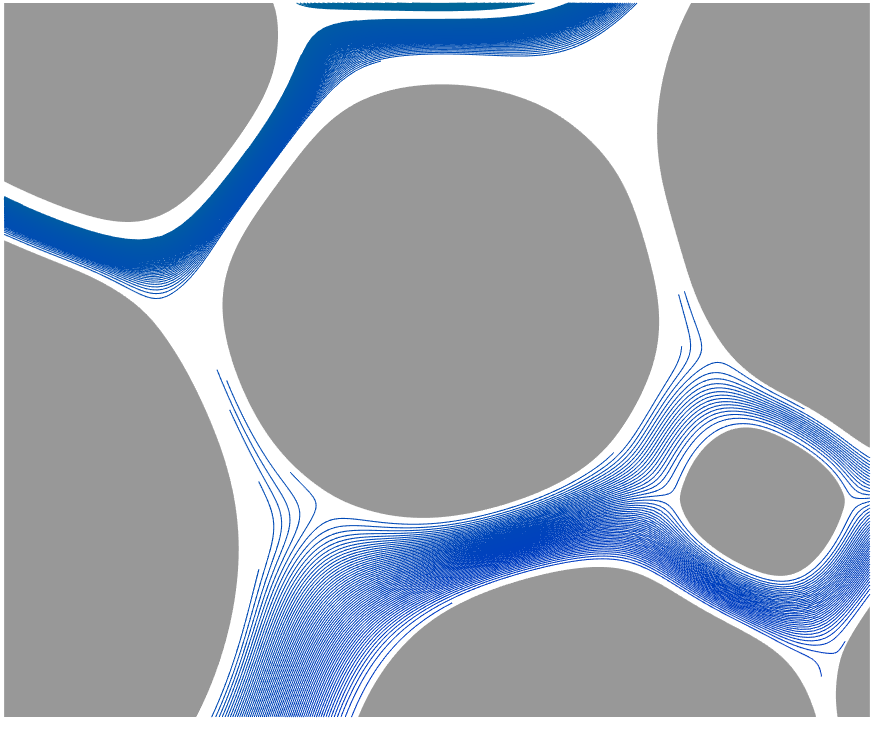
\includegraphics[width = 0.32\textwidth]{./figs/tracer_20b210_zoom}
%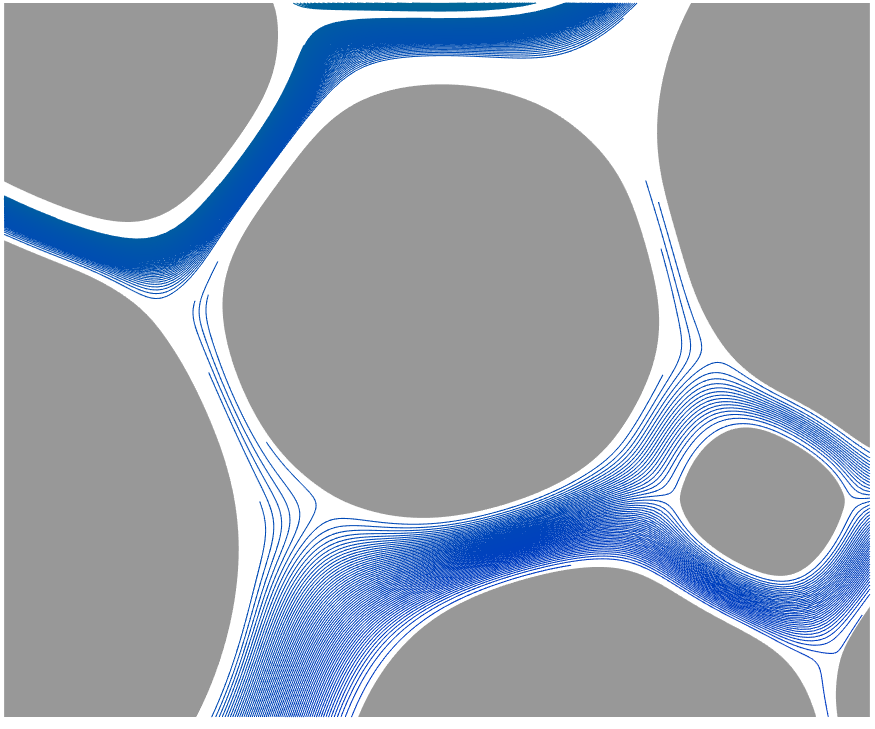
\includegraphics[width = 0.32\textwidth]{./figs/tracer_20b240_zoom}
%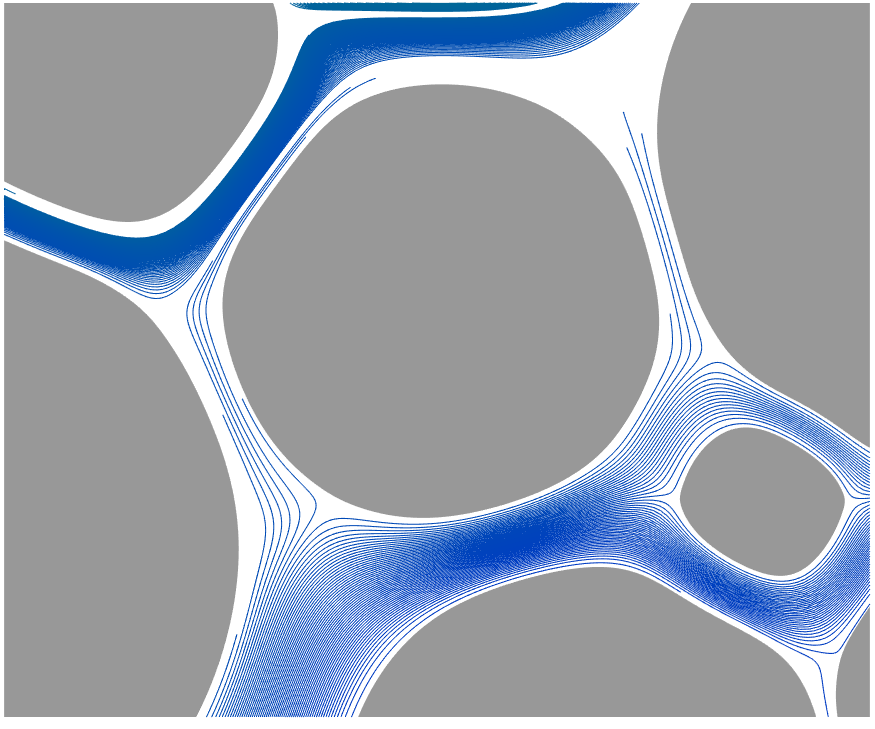
\includegraphics[width = 0.32\textwidth]{./figs/tracer_20b270_zoom}
%\caption{\label{fig:Eroding20zoom}The zoom windows in the last three
%  frames of Figure~\ref{fig:Eroding20tracer}. The trajectories of
%  tracers around the bodies. Since we use a Barycentric quadrature rule
 % and the fourth order Runge Kutta method, the tracers can be very close
 % to but not penetrate the bodies.}
%\end{center}
%\end{figure}
%{\color{red}
%In Fig.~\ref{fig:Eroding20tort} we release 1000 tracers 
%from the starting cross section x = -1 to 
%the end cross section x = 1 and 
%use the local tortuosity to analysis the effect
%of the geometrical structure on fluid velocity field when the porosity is 62.9 \%.
%In Fig.~\ref{fig:Eroding20tort}(a) the graph represents the ratio of the
%x-component velocity u(-1, y) to its maximum velocity $u_{max}=2.9828
%\times 10^{-3}$ at equal spreading tracers on the starting cross section.
%The velocity is continuous along the starting cross section and
%acting as several Poiseuille flows. This velocity graph is different
%from the one in~\cite{matyka2008tortuosity} since we choose our cross
%section to be the beginning of the flow before the fluid touches any
%body. In Fig.~\ref{fig:Eroding20tort}(b) we record the local tortuosity
%$\tau(y)=\lambda(y)/d$
%of the tracers at $y$ on the starting cross section x = -1 
%where $d = 2$.
%This graph is not continuous 
%and the jumps in $\tau$ mean that the initial neighboring tracers have been
%seperated by the bodies. 
%The maximum of $\tau$ is 1.2713 and the minimum is 1.0001.
%}
%{\color{red}
%In Fig.~\ref{fig:Eroding20tort}(c) we calculate the difference of 
%$\tau$ at two neighboring tracers 
%and draw the trajectories of neighboring tracers
%if the difference of $\tau$ at the neighboring tracers is large. 
%From Fig.~\ref{fig:Eroding20tort}(c), we collect the 10 largest difference of $\tau$ 
%at the neighboring tracers and 
%draw the pair of trajectories in the same color and 
%are able to tell the neighboring trajectories will be very 
%different if they are separated by bodies.
%For each pair of trajectories, 
%they are splitted by the body at the left side of the body, then
%one of them goes up and the other one goes down along the body 
%until they rejoin with each other at the right side of body.  
%Furthermore, the pair trajectories could be splitted by more than one body, 
%for example in Fig.~\ref{fig:Eroding20tort}(c) the toppest red pair trajectories 
%are splitted by two close bodies.
%}

%To measure the local behavior of fluid quantitatively, 
%we use the velocities and local tortuosities at the starting cross section 
%to analysis the interaction of fluid and bodies until the end cross section 
%in Fig.~\ref{fig:Eroding100tort}(b) and (c).
%In Fig.~\ref{fig:Eroding100tort}(b) the graph represents the ratio of the
%x-component velocity u(-1, y) to its maximum velocity $u_{max}=3.9021
%\times 10^{-4}$ at equal spreading tracers on the strating cross section.
%As in the case of 20 nearly touching bodies, the velocity is continuous along
%the starting cross section and acting as a Poiseuille flow in the channel between
%bodies. When the fluid is close to bodies
%the speed of fluid will be slow down because of the no-slip condition on the bodies
%and this causes the separated branches of the inlet flow.
%The maximum velocity of the fluid with 100 bodies on the starting cross 
%section is slower than the maximum velocity of the fluid with 20 bodies
%but the velocity in the case of 100 bodies 
%changes more rapidly than the velocity of the fluid with 20 bodies.
%The reason of the rapid change on the starting cross section of 
%100-body case is because there are 
%more bodies near the starting cross section in
%100-body case than in the 20-body case. 
%so the inlet flow in 100-body case
%will be separated into more branches than the flow in 20-body case. 
%
%In Fig.~\ref{fig:Eroding100tort}(c) we record the 
%local tortuosity $\tau(y)$ for $y$ on the starting cross section x = -1.
%It is a discontinous function and the maximum of $\tau$ in the case of 100 bodies
%is 1.2547 and the minimum is 1.0003. This function $\tau$
%has more jumps than the one in the case of 20 bodies but its maximum 
%is smaller than the maximum in the case of 20 bodies. 
%The jump in this graph means the neighboring trajectories are splitted by bodies
%so it is reasonable to have more jumps in the case of 100-body than the case of 20-body
%since there are more bodies in the former case. 

%To study the behavior of fluid in the porous media with multiple bodies, 
%we release 1000 tracers equispaced in $y$ from the 
%cross section x = -1 and record their trajectories and velocities
%until they arrive the end cross section x = 1 
%and the porosity of this geometric structure is 62.98 \%. 
%To understand the global action of fluid qualitatively, 
%we only draw 200 historical trajectories from x = -1 to x = 1 
%in Fig.~\ref{fig:Eroding100tort}(a). 
%When equispaced tracers are released in a 2D tube without any grains, 
%the streamlines are straight 
%and the intersection points of streamlines and any cross section are equispaced. 
%But it is not the same when there are bodies in the fluid. 
%In Fig.~\ref{fig:Eroding100tort}(a)
%even the tracers are equispaced in $y$ on the cross section $S$, 
%the streamlines have been push up and down by the bodies and
%some of them are close together. 
%
%
%%To understand the meaning of jump 
%%of $\tau$, we use the data we got from local tortuosity $\tau(y)$
%%to find the difference of $\tau$ at the neighboring tracers in Fig.~\ref{fig:Eroding100tort}(c) 
%%and draw 50 pairs of neighboring trajectories which have the largest difference of $\tau$
%%in Fig.~\ref{fig:Eroding100tort_traj}. These pairs of two neighboring trajectories are splitted by bodies
%%then rejoin with each other and the splitting-rejoining behavior causes the difference of $\tau$ with respect to the neighboring trajectories.   
%%We also can get the idea why the maximum value of $\tau$ is smaller 
%%than the one in the case of 20 bodies . 
%%The most of the bodies in this case are smaller than those in the case of 20 bodies.
%%So when two neighboring trajectories are splitted on the left side by a smaller body they do not
%%travel as far as the two splitted by a bigger body do after they rejoin on the right side. 


%{\color{red}
%This case is 100 bodies in a Hagen-Poiseuille flow. The background
%flow is 
%\begin{align}
%  \UU(\xx)=U \left[
%  \begin{array}{c}
%    1-y^2 \\ 0
%  \end{array}
%  \right]
%\end{align}
%with floating flow rate $U$ such that pressure drop is fixed from x = -2 to x = 2.
%We record the vorticity of 
%fluid in colormap during the bodies erosion in Fig.~\ref{fig:Eroding100vort} and 
%measure the gap sizes between bodies in Fig.~\ref{fig:Eroding100gap} at four equispaced times.
%Since the vorticity is equivalent to the shear stress and the erosion is faster in the regions where
%the magnitude of the vorticity is larger 
%so the erosion is getting faster and faster 
%from the first snapshot to the forth one in Fig.~\ref{fig:Eroding100vort}.
%At t = 0.005 the porosity is 55.54\% and the most gap sizes between bodies are less than 0.015 in 
%Fig.~\ref{fig:Eroding100gap}(a). Since some of the bodies are vanished in the fluid, the numner of gaps 
%decreases and the gap sizes get larger and larger between the remaining bodies. 
%In Fig.~\ref{fig:Eroding100gap}(b) and (c) we still can see small gap sizes are in the majority but 
%it is not as concentrated as the one we see in Fig.~\ref{fig:Eroding100gap}(a). 
%In Fig.~\ref{fig:Eroding100gap}(d) there are only 254 gaps between 82 bodies and 
%the distribution of gap sizes spreads over without any major pack.  
%}
%
%\begin{figure}[H]
%\center
%\includegraphics*[width = 0.55\linewidth]{./figs/tort_eulerian}
%\caption{\label{fig:Eroding20tort_all} The tortuosity inside of an
%eroding geometry initialized with 20 bodies.  The tortuosity is
%calculated using the Eulerian method~\eqref{eqn:tortuosity2} (blue dots)
%and Lagrangian method~\eqref{eqn:tortuosity1} (red stars).  The red
%square correspond to the geometry in Figure~\ref{fig:Eroding20tort}(c).
%The dash line is the fitting line $\widehat{T}(\phi)=\phi^{-p}$ as
%$p=0.2064$ and the root-mean-square error is $5.9 \times 10^{-3}$.}
%\end{figure}
%
%
%\begin{figure}[H]
%\center
%\includegraphics*[width =0.55\linewidth]{./figs/20b_second_moment_long_ref}
%\caption{\label{fig:Eroding20anomalousMedium} The analysis of anomalous
%dispersion in 20 nearly touching bodies with respect to initial porosity
%(as p=37.68\%) and another six porosities during the eroding. The dashed
%line correspondes to a porosity of 100\% and the dashed-dotted lines are
%lines of best fit with slope 1.0644 (as p=95.1\%), 1.0673 (as
%p=85.09\%), 1.0594 (as p=75.15\%), 0.9664 (as p=65.09\%), 0.7766 (as
%p=55.10\%), 0.7475 (as p=45.08\%), and 0.5607 (as p=37.68\%.}
%\end{figure}
%

%\begin{figure}[H]
%\center
%\includegraphics*[width =0.55\linewidth]{./figs/tort_eulerian20b}
%\caption{\label{fig:ErodingLow20tort} The tortuosity inside of an
%eroding geometry initialized with 20 bodies.  The tortuosity is
%calculated using the Eulerian method~\eqref{eqn:tortuosity2} (blue
%dots).  The dash line is the fitting line $\widehat{T}(\phi)=\phi^{-p}$
%as $p=0.1669$ and the root mean square deviation is $1.13 \times
%10^{-2}$.}
%\end{figure}
%
%\begin{figure}[H]
%\center
%\includegraphics*[width =0.55\linewidth]{./figs/20b_dense_second_moment_ref}
%\caption{\label{fig:Eroding20anomalousLow} The analysis of anomalous
%dispersion in 20 nearly touching bodies with respect to initial porosity
%(as p=30.67\%) and another seven porosities during the eroding. The
%dashed line correspondes to a porosity of 100\% and the dashed-dotted
%lines are lines of best fit with slope 0.9194 (as p=95\%), 0.8666 (as
%p=85.17\%), 0.8682 (as p=75.10\%), 0.9087 (as p=65.02\%), 0.9054 (as
%p=55.08\%), 0.7234 (as p=45.03\%), 0.6895 (as p=35.05\%), and 0.9225 (as
%p=30.67\%).}
%\end{figure}


\end{document}


